\PassOptionsToPackage{unicode=true}{hyperref} % options for packages loaded elsewhere
\PassOptionsToPackage{hyphens}{url}
%
\documentclass[12pt,a4paper,UTF8,twoside]{book}

\usepackage{lmodern}
\usepackage{setspace}
\setstretch{1.25}
\usepackage{amssymb,amsmath}
\usepackage{ifxetex,ifluatex}
\usepackage{fixltx2e} % provides \textsubscript
\ifnum 0\ifxetex 1\fi\ifluatex 1\fi=0 % if pdftex
  \usepackage[T1]{fontenc}
  \usepackage[utf8]{inputenc}
\else % if luatex or xelatex
  \ifxetex
    \usepackage{xltxtra,xunicode}
  \else
    \usepackage{fontspec}
  \fi
  \defaultfontfeatures{Mapping=tex-text,Scale=MatchLowercase}
  \newcommand{\euro}{€}

    \setmainfont[]{Times New Roman}
    \setsansfont[]{Arial}
    \setmonofont[Mapping=tex-ansi]{Inconsolata}
\fi

% use upquote if available, for straight quotes in verbatim environments
\IfFileExists{upquote.sty}{\usepackage{upquote}}{}
% use microtype if available
\IfFileExists{microtype.sty}{%
\usepackage[]{microtype}
\UseMicrotypeSet[protrusion]{basicmath} % disable protrusion for tt fonts
}{}
\usepackage{hyperref}
\hypersetup{
            pdftitle={Master Thesis Template},
            pdfauthor={Xiang-Yun Huang},
            pdfproducer={Pandoc, R Markdown, TinyTeX, knitr, bookdown, Stan},
            pdfborder={0 0 0},
            breaklinks=true}
\urlstyle{same}  % don't use monospace font for urls
\usepackage[margin=1.18in]{geometry}
\usepackage{longtable,booktabs}
% Fix footnotes in tables (requires footnote package)
\IfFileExists{footnote.sty}{\usepackage{footnote}\makesavenoteenv{longtable}}{}
\usepackage{graphicx,grffile}
\makeatletter
\def\maxwidth{\ifdim\Gin@nat@width>\linewidth\linewidth\else\Gin@nat@width\fi}
\def\maxheight{\ifdim\Gin@nat@height>\textheight\textheight\else\Gin@nat@height\fi}
\makeatother
% Scale images if necessary, so that they will not overflow the page
% margins by default, and it is still possible to overwrite the defaults
% using explicit options in \includegraphics[width, height, ...]{}
\setkeys{Gin}{width=\maxwidth,height=\maxheight,keepaspectratio}
\setlength{\emergencystretch}{3em}  % prevent overfull lines
\providecommand{\tightlist}{%
  \setlength{\itemsep}{0pt}\setlength{\parskip}{0pt}}
\setcounter{secnumdepth}{5}
% Redefines (sub)paragraphs to behave more like sections
\ifx\paragraph\undefined\else
\let\oldparagraph\paragraph
\renewcommand{\paragraph}[1]{\oldparagraph{#1}\mbox{}}
\fi
\ifx\subparagraph\undefined\else
\let\oldsubparagraph\subparagraph
\renewcommand{\subparagraph}[1]{\oldsubparagraph{#1}\mbox{}}
\fi

% set default figure placement to htbp
\makeatletter
\def\fps@figure{htbp}
\makeatother

\usepackage[UTF8, heading]{ctex}
\usepackage{amssymb,amsmath,amsfonts,mathrsfs}
\setCJKmainfont[ItalicFont={KaiTi_GB2312}, BoldFont={SimHei}]{SimSun}
\setCJKsansfont{SimHei}
\setCJKmonofont{FangSong_GB2312}
\usepackage{color}
\ctexset{
  chapter/name = {,},
  chapter/number = \arabic{chapter},
  chapter/numberformat = \sf,
  chapter/beforeskip = 12pt,
  chapter/afterskip = 18pt,
  chapter/fixskip = true,
  chapter/format += \sf\zihao{3},
  section/numberformat = \rm,
  section/format += \sf\zihao{4}\raggedright,
  section/beforeskip = 16pt,
  section/afterskip = 16pt,
  section/fixskip = true,
  subsection/numberformat = \rm,
  subsection/format += \sf\zihao{-4}\raggedright,
  subsection/fixskip = true,
  subsection/beforeskip = 16pt,
  subsection/afterskip = 16pt,
  subsubsection/numberformat = \rm,
  subsubsection/format += \sf\zihao{-4}\raggedright,
  contentsname = {目\quad 录},
}

\usepackage[titles]{tocloft}
\renewcommand{\cftdot}{$\ldotp$}
\renewcommand{\cftdotsep}{0}
\renewcommand{\cftchapleader}{\cftdotfill{\cftchapdotsep}}
\renewcommand{\cftchapdotsep}{\cftdotsep}

\usepackage[lotdepth=2,lofdepth=2]{subfig}

\usepackage{fancyhdr}
\pagestyle{fancy}
\fancyhf{}
\renewcommand{\headrule}{\hrule height1pt width\headwidth \vspace{3.0pt}\hrule width\headwidth}
\fancyhead[EC]{\kaishu \zihao{5}中国矿业大学(北京)硕士学位论文}
\fancyhead[OC]{\kaishu \zihao{5}\leftmark}
\fancyfoot[C]{\thepage}

\fancypagestyle{plain}{ \fancyhf{}
\fancyhead[EC]{\kaishu\zihao{5} 中国矿业大学(北京)硕士学位论文}
\fancyhead[OC]{\kaishu\zihao{5} \leftmark}
\fancyfoot[C]{\thepage}}

\usepackage{array}
\usepackage{multirow}
\usepackage[table]{xcolor}
\usepackage{wrapfig}
\usepackage{float}
\usepackage{colortbl}
\usepackage{pdflscape}
\usepackage{tabu}
\usepackage{threeparttable}
\usepackage{threeparttablex}
\usepackage[normalem]{ulem}
\usepackage{makecell}

\frontmatter

\usepackage[super,square,sort]{natbib}
\bibliographystyle{GBT7714-2005}


\title{Master Thesis Template}
\providecommand{\subtitle}[1]{}
\subtitle{China University of Mining and Technology, Beijing}
\author{Xiang-Yun Huang}
\date{2018-10-24}

\usepackage{amsthm}
\newtheorem{theorem}{定理}[chapter]
\newtheorem{lemma}{引理}[chapter]
\newtheorem{corollary}{推论}[chapter]
\newtheorem{proposition}{命题}[chapter]
\newtheorem{conjecture}{Conjecture}[chapter]
\theoremstyle{definition}
\newtheorem{definition}{定义}[chapter]
\theoremstyle{definition}
\newtheorem{example}{例}[chapter]
\theoremstyle{definition}
\newtheorem{exercise}{练习}[chapter]
\theoremstyle{remark}
\newtheorem*{remark}{Remark}
\newtheorem*{solution}{Solution}
\let\BeginKnitrBlock\begin \let\EndKnitrBlock\end
\begin{document}
% \maketitle

\input{latex/00a-cover.tex}  % 封面

\input{latex/00b-titlepage.tex}  % 标题

\input{latex/00c-declaration.tex}  % 声明

\input{latex/00d-abstract.tex}  % 摘要

{
\setcounter{tocdepth}{2}
\tableofcontents
}

\mainmatter

\hypertarget{intro}{%
\chapter{绪论}\label{intro}}

空间统计的内容非常丰富,主要分为地质统计 (geostatistics)、
离散空间变差 (discrete spatial variation) 和空间点过程 (spatial point
processes) 三大块 \citep{Cressie1993}。
地质统计这个术语最初来自南非的采矿业 \citep{Krige1951}, 并由 Georges
Matheron
及其同事继承和发展,用以预测黄金的矿藏含量和质量。空间广义线性混合效应模型
(Spatial Generalized Linear Mixed Model,简称 SGLMM)
在空间统计中有着广泛的应用,如评估岩心样本石油含量,分析核污染物浓度的空间分布
\citep{Diggle1998}, 预测冈比亚儿童疟疾流行度的空间分布
\citep{Diggle2002Childhood},
喀麦隆及其周边地区的热带眼线虫流行病的的空间分布
\citep{Diggle2007ATMP},对热带疾病预防和控制项目提供决策支持
\citep{Schl2016Using}。
在热带地区,淋巴丝虫病和盘尾丝虫病是严峻的公共卫生问题,
据世界卫生组织统计, 在非洲撒哈拉以南、 阿拉伯半岛和南美洲的 34 个国家约
2000 \textasciitilde{} 4000 万人感染河盲病 \citep{Takougang2002Rapid}。
例如, 喀麦隆中部省份 Loa loa
是导致河盲病的寄生虫,它的感染强度与疾病流行度之间存在线性关系, 即 Loa
loa 感染强度越大流行度越高 \citep{Boussinesq2001}。 1997 年,研究表明
Loa loa 流行度对应的高感染强度的临界值为 20\%
\citep{Gardon1997Serious},
而研究个体水平的感染情况与群体水平流行度之间的关系有助于大规模给药
\citep{Schl2016Using},所以更加高效的算法和算法实现可以更快、更准、更有效地在大范围内做疾病预防和医疗资源分配。

\hypertarget{reviews}{%
\section{文献综述}\label{reviews}}

如何计算空间广义线性混合效应模型的参数一直以来是研究的重点,由于模型中的随机效应和空间位置相关联,而空间位置的数量和具体坐标直接影响空间效应的维度,给参数估计值的计算带来很大的复杂性,因为参数的贝叶斯估计和极大似然估计都离不开对空间效应的高维积分,所以在计算上是一个很大的挑战。在贝叶斯方法下,Diggle
等 (1998 年) \citep{Diggle1998} 提出随机游走的 Metropolis
程序实现马尔科夫链蒙特卡罗算法获得模型参数的后验密度分布及后验量的估计值。Ribeiro
和 Diggle (2001 年) \citep{geoR2001} 提出 Langevin-Hastings
算法,相比于随机游走的 Metropolis
算法,取得了更好的计算效率,后续的一个稳健版本由 Christensen (2006 年)
\citep{Christensen2006} 给出。在实际操作中,马尔科夫链蒙特卡罗算法(简称
MCMC)面临的主要问题是收敛性诊断和计算时间,
当然算法实现的本身也很重要,对终端用户来说,可能大部分并不善于编程,所以算法的实现过程可能存在问题,因此,寻求一个好的贝叶斯推断工具或平台也很重要。目前,通过
MCMC 方式拟合带随机效应的模型有
\href{http://www.mrc-bsu.cam.ac.uk/software/bugs/the-bugs-project-winbugs/}{WinBUGS},\href{http://www.openbugs.net/}{OpenBUGS},
\href{http://mcmc-jags.sourceforge.net/}{JAGS},\href{http://www.BayesX.org}{BayesX},
\href{https://www.multibugs.org}{MultiBUGS},\href{https://r-nimble.org/}{NIMBLE},Stan
\citep{Stan2017JSS}
等软件。近年来,一些研究者开始将注意力放到高维积分的近似上,从而出现了一类新的近似贝叶斯推断,
Rue 等 (2009 年) \citep{Rue2009}
在高斯马尔科夫随机场近似平稳空间高斯过程的设置下,用拉普拉斯近似空间效应的高维积分,从而提出集成嵌套拉普拉斯算法,Lindgren
等 (2011 年) \citep{Lindgren2011}
提出相似的算法用于随机效应是偏态分布情形下的 SGLMM 模型的参数估计。Rue
等 (2009 年) \citep{Rue2009}
肯定了拉普拉斯近似方法的使用,认为这类近似具有足够的准确度,可以用于实际数据分析。虽然在计算上达到了快捷,但人们对贝叶斯方法最严厉的评判依然是它依赖于先验分布的选择。
Christensen (2004 年) \citep{Christensen2004}
又提出蒙特卡罗极大似然算法,它还是依赖 MCMC
算法,但是提供了关于参数的似然分析,其算法实现打包在 R 包 geoRglm
里,详细描述参见 Diggle 和 Ribeiro(2007 年)
\citep{Diggle2007}。作为蒙特卡罗似然的一个替代方法, Hao (2002
年)\citep{Zhang2002On} 提出蒙特卡罗期望极大算法 (简称 MCEM
),他将不能直接观察到的空间随机效应部分看作是缺失数据。

Diggle 等 (1998 年) \citep{Diggle1998}基于马绍尔群岛国家放射性调查数据
--- 记录南太平洋朗格拉普岛上 \({}^{137}\mathrm{Cs}\) 放射 \(\gamma\)
粒子的强度数据,建立响应变量服从泊松分布的 SGLMM
模型,在贝叶斯方法下,用 Metropolis-Hastings 采样实现 MCMC 算法,获得
SGLMM
模型的参数估计,分析了残留的核污染物浓度的空间分布,此外,他们还建立响应变量服从二项分布的
SGLMM 模型分析北拉纳克郡和南坎布里亚郡的居民感染弯曲杆菌的空间分布情况。
Christensen (2004 年) \citep{Christensen2004} 在 Diggle 等 (1998 年)
\citep{Diggle1998}
分析格拉普岛核残留数据的模型上,添加非空间的相互独立的随机效应,取得了更好的拟合效果,这种非空间的随机效应在地质统计学中常称为块金效应(nugget
effect)。Diggle 和 Giorgi (2016年) \citep{Diggle2016}
基于肯尼亚尼扬扎省的疟疾数据,该数据组合了学校和村庄的信息,分析的是一个多源数据,假定其中一个数据是有偏的,来自非随机的调查,另一个数据是无偏的,来自随机调查,因而建立包含两个服从平稳空间过程的空间随机效应,使用蒙特卡罗极大似然算法(简称
MCML )估计二项 SGLMM
模型的参数,获得疟疾在该省的空间分布;第二个数据是马拉维奇瓦瓦区 2010 年
5 月至 2013 年 6 月收集的疟疾数据,在 Diggle 等 (1998 年)
\citep{Diggle1998}的基础上将时间考虑进二项 SGLMM
模型中,并且假定时间项和空间项是无关的,而块金效应只依赖于时间变化,同样基于
MCML 算法,估计了模型的各个参数;第三个数据建模是在带块金效应的 SGLMM
基础上,认为响应变量应服从混合二项分布以包含极低的感染程度,比如有些村庄没有一个受到感染,因此建立零过多
(Zero-inflation)二项空间混合效应模型分析第三个河盲病数据集。

在面对复杂的高维积分时,每种替代方法,无论走随机模拟还是近似的路线,都有相应的代价,基于拉普拉斯近似的方法依赖于初值的选择,基于随机模拟的
MCMC
算法依赖于先验分布和算法参数的调整,这些对最后的数据分析结果都会产生影响,调参的过程往往充满经验和技巧。尽管不断有新的、复杂的算法和方法开发出来,Bonat
和 Ribeiro(2016年) \citep{Bonat2016Practical}
认为只有能被广泛使用,实现方式比较直接的参数估计方法才是比较安全可靠的选择。

\hypertarget{stracture}{%
\section{论文结构}\label{stracture}}

第 \ref{intro} 章绪论部分介绍了 SGLMM 模型的研究现状, 综述了 SGLMM
模型参数估计的贝叶斯 MCMC 和 MCML等算法及其应用情况。

第 \ref{prepare}
章介绍了指数族,最小二乘估计,极大似然估计,平稳高斯过程,拉普拉斯近似,先验和后验分布和蒙特卡罗积分等基础知识,它们作为后续相关章节的知识准备。

第 \ref{models} 章回顾了一般线性模型到 SGLMM 模型的结构,
指出了模型从简单到复杂的变化过程,及其中的区别和联系。

第 \ref{algorithms} 章首先介绍了目前估计 SGLMM
模型参数的算法,依次是拉普拉斯近似算法、蒙特卡罗极大似然算法、贝叶斯
MCMC 算法和低秩近似算法,并在 Langevin-Hastings 算法的基础上,我们提出
Stan 程序库实现的汉密尔顿蒙特卡罗算法(简称
HMC),在文中为了方便,也称作贝叶斯 STAN-MCMC 算法。

第 \ref{simulations}
章首先介绍了一维和二维情形下平稳空间高斯过程的模拟,然后在二维情形下,分别模拟了响应变量服从二项分布和泊松分布的
SGLMM 模型,比较了贝叶斯 MCMC 算法和我们提出的贝叶斯 STAN-MCMC
算法,结论是在获得相似估计效果的情形下,我们提出的算法迭代次数少。

第 \ref{applications}
章给出了两个案例分析,分别是基于空间线性混合效应模型的小麦数据分析和基于泊松型空间广义线性混合效应模型的核污染数据分析,我们发现基于样本变差图和剖面似然轮廓的可视化辅助手段可以获得非常好的模型参数初始值。

第 \ref{summary} 章总结论文的主要工作、相关结论和后续研究方向。

\hypertarget{prepare}{%
\chapter{基础知识}\label{prepare}}

作为第 \ref{models} 章统计模型和第 \ref{algorithms}
章参数估计的知识准备,本章给出主要的知识点。第 \ref{sec:exp}
节首先介绍指数族的一般形式,包含各成分的定义,特别给出正态分布、二项分布和泊松分布情形下均值函数、联系函数和方差函数等特征量。第
\ref{sec:lse}
节给出线性模型下,设计矩阵保持正定时的最小二乘估计和加权最小二乘估计。第
\ref{sec:def-mle}
节给出极大似然估计的定义,相合性,以及在一定条件下的渐近正态性。第
\ref{sec:stationary-gaussian-process}
节给出平稳高斯过程的定义,均方连续性和可微性的定义,以及判断可微性的一个充要条件。第
\ref{sec:Laplace-approximation} 节介绍了拉普拉斯近似的一般方法。第
\ref{sec:bayes-prior} 介绍了先验、后验分布和 Jeffreys 无信息先验分布。第
\ref{sec:stan-samplers} 节首先从 Stan
的发展、内置算法设置以及与同类软件的比较等三方面介绍,然后以数据集 Eight
Schools 为例子介绍 Stan 的使用,为空间广义线性混合效应模型的 Stan
实现作铺垫。

\hypertarget{sec:exp}{%
\section{指数族}\label{sec:exp}}

一般地,样本 \(\mathbf{Y}\) 的分布服从指数族,即形如 \begin{equation}
f_{Y}(y;\theta,\phi) = \exp\big\{ \big(y\theta - b(\theta) \big)/a(\phi) + c(y,\phi) \big\}
\label{eq:common-exponential-family}
\end{equation} \noindent 其中,\(a(\cdot),b(\cdot),c(\cdot)\)
是某些特定的函数。如果 \(\phi\) 已知,这是一个含有典则参数 \(\theta\)
的指数族模型,如果 \(\phi\)
未知,它可能是含有两个参数的指数族。对于正态分布 \begin{equation}
\begin{aligned}
f_{Y}(y;\theta,\phi) & = \frac{1}{\sqrt{2\pi\sigma^2}} \exp\{-\frac{(y - \mu)^2}{2\sigma^2}  \}  \\
 & = \exp\big \{ (y\mu - \mu^2/2)/\sigma^2 - \frac{1}{2}\big(y^2/\sigma^2 + \log(2\pi\sigma^2)\big) \big\}
\end{aligned} \label{eq:normal-distribution}
\end{equation} \noindent 通过与 \eqref{eq:common-exponential-family}
式对比,可知 \(\theta = \mu\),\(\phi = \sigma^2\),并且有 \[
a(\phi) = \phi, \quad b(\theta) = \theta^2/2, \quad c(y,\phi) = - \frac{1}{2}\{ y^2/\sigma^2 + \log(2\pi\sigma^2) \} 
\] \noindent 记 \(l(\theta,\phi;y) = \log f_{Y}(y;\theta,\phi)\)
为给定样本点 \(y\) 的情况下,关于 \(\theta\) 和 \(\phi\)
的对数似然函数。样本 \(Y\) 的均值和方差具有如下关系 \begin{equation}
\mathsf{E}\big( \frac{\partial l}{\partial \theta} \big) = 0
\label{eq:mean-log-lik}
\end{equation} \noindent 和 \begin{equation}
\mathsf{E}\big( \frac{\partial^2 l}{\partial \theta^2} \big) + \mathsf{E}\big(\frac{\partial l}{\partial \theta}\big)^2  = 0
\label{eq:variance-log-lik}
\end{equation} \noindent 从 \eqref{eq:common-exponential-family} 式知
\[ l(\theta,\phi;y) = {y\theta - b(\theta)}/a(\phi) + c(y,\phi) \]
\noindent 因此, \begin{equation}
\begin{aligned}
\frac{\partial l}{\partial \theta} & = {y - b'(\theta)}/a(\phi)  \\
\frac{\partial^2 l}{\partial \theta^2}  & = - b''(\theta)/a(\phi)
\end{aligned} \label{eq:partial-log-lik}
\end{equation} \noindent 从 \eqref{eq:mean-log-lik} 式和
\eqref{eq:partial-log-lik},可以得出 \[ 
0 = \mathsf{E}\big( \frac{\partial l}{\partial \theta} \big) = \big\{ \mu - b'(\theta) \big\}/a(\phi)
\] \noindent 所以 \[ \mathsf{E}(Y) = \mu = b'(\theta) \] \noindent 根据
\eqref{eq:variance-log-lik} 式和 \eqref{eq:partial-log-lik} 式,可得
\[ 0 = - \frac{b''(\theta)}{a(\phi)} + \frac{\mathsf{Var}(Y)}{a^2(\phi)} \]
\noindent 所以 \[ \mathsf{Var}(Y) = b''(\theta)a(\phi) \] 可见,\(Y\)
的方差是两个函数的乘积,一个是 \(b''(\theta)\),
它仅仅依赖典则参数,叫做方差函数,方差函数可以看作是 \(\mu\)
的函数,记作 \(V(\mu)\)。另一个是 \(a(\phi)\),它独立于
\(\theta\),仅仅依赖 \(\phi\),函数 \(a(\phi)\) 通常形如
\[ a(\phi) = \phi/w \] \noindent 其中 \(\phi\) 可由 \(\sigma^2\)
表示,故而也叫做发散参数 (dispersion
parameter),是一个与样本观察值相关的常数,\(w\)
是已知的权重,随样本观察值变化。对正态分布模型而言,\(w\) 的分量是 \(m\)
个相互独立的样本观察值的均值,有
\(a(\phi) = \sigma^2/m\),所以,\(w = m\)。

根据
\eqref{eq:common-exponential-family}式,正态、泊松和二项分布的特征见表
\ref{tab:common-characteristics},其它常见分布见 McCullagh 等 (1989年)
\citep{McCullagh1989}。

\begin{longtable}[]{@{}lccc@{}}
\caption[\label{tab:common-characteristics}
指数族内常见的一元分布的共同特征及符号表示]{\label{tab:common-characteristics}
指数族内常见的一元分布的共同特征及符号表示\footnotemark{}}\tabularnewline
\toprule
\begin{minipage}[b]{0.21\columnwidth}\raggedright
\strut
\end{minipage} & \begin{minipage}[b]{0.22\columnwidth}\centering
正态分布\strut
\end{minipage} & \begin{minipage}[b]{0.22\columnwidth}\centering
泊松分布\strut
\end{minipage} & \begin{minipage}[b]{0.22\columnwidth}\centering
二项分布\strut
\end{minipage}\tabularnewline
\midrule
\endfirsthead
\toprule
\begin{minipage}[b]{0.21\columnwidth}\raggedright
\strut
\end{minipage} & \begin{minipage}[b]{0.22\columnwidth}\centering
正态分布\strut
\end{minipage} & \begin{minipage}[b]{0.22\columnwidth}\centering
泊松分布\strut
\end{minipage} & \begin{minipage}[b]{0.22\columnwidth}\centering
二项分布\strut
\end{minipage}\tabularnewline
\midrule
\endhead
\begin{minipage}[t]{0.21\columnwidth}\raggedright
记号\strut
\end{minipage} & \begin{minipage}[t]{0.22\columnwidth}\centering
\(\mathcal{N}(\mu,\sigma^2)\)\strut
\end{minipage} & \begin{minipage}[t]{0.22\columnwidth}\centering
\(\mathrm{Poisson}(\mu)\)\strut
\end{minipage} & \begin{minipage}[t]{0.22\columnwidth}\centering
\(\mathrm{Binomial}(m,\pi)/m\)\strut
\end{minipage}\tabularnewline
\begin{minipage}[t]{0.21\columnwidth}\raggedright
\(y\) 取值范围\strut
\end{minipage} & \begin{minipage}[t]{0.22\columnwidth}\centering
\((-\infty,\infty)\)\strut
\end{minipage} & \begin{minipage}[t]{0.22\columnwidth}\centering
\(0(1)\infty\)\strut
\end{minipage} & \begin{minipage}[t]{0.22\columnwidth}\centering
\(0(1)m\)\strut
\end{minipage}\tabularnewline
\begin{minipage}[t]{0.21\columnwidth}\raggedright
\(\phi\)\strut
\end{minipage} & \begin{minipage}[t]{0.22\columnwidth}\centering
\(\phi = \sigma^2\)\strut
\end{minipage} & \begin{minipage}[t]{0.22\columnwidth}\centering
\(1\)\strut
\end{minipage} & \begin{minipage}[t]{0.22\columnwidth}\centering
\(1/m\)\strut
\end{minipage}\tabularnewline
\begin{minipage}[t]{0.21\columnwidth}\raggedright
\(b(\theta)\)\strut
\end{minipage} & \begin{minipage}[t]{0.22\columnwidth}\centering
\(\theta^2/2\)\strut
\end{minipage} & \begin{minipage}[t]{0.22\columnwidth}\centering
\(\exp(\theta)\)\strut
\end{minipage} & \begin{minipage}[t]{0.22\columnwidth}\centering
\(\log(1+e^{\theta})\)\strut
\end{minipage}\tabularnewline
\begin{minipage}[t]{0.21\columnwidth}\raggedright
\(c(y;\theta)\)\strut
\end{minipage} & \begin{minipage}[t]{0.22\columnwidth}\centering
\(-\frac{1}{2}\big( \frac{y^2}{\phi} + \log(2\pi\phi) \big)\)\strut
\end{minipage} & \begin{minipage}[t]{0.22\columnwidth}\centering
\(-\log(y!)\)\strut
\end{minipage} & \begin{minipage}[t]{0.22\columnwidth}\centering
\(\log\binom{m}{my}\)\strut
\end{minipage}\tabularnewline
\begin{minipage}[t]{0.21\columnwidth}\raggedright
\(\mu(\theta) = \mathsf{E}(Y;\theta)\)\strut
\end{minipage} & \begin{minipage}[t]{0.22\columnwidth}\centering
\(\theta\)\strut
\end{minipage} & \begin{minipage}[t]{0.22\columnwidth}\centering
\(\exp(\theta)\)\strut
\end{minipage} & \begin{minipage}[t]{0.22\columnwidth}\centering
\(e^{\theta}/(1+e^{\theta})\)\strut
\end{minipage}\tabularnewline
\begin{minipage}[t]{0.21\columnwidth}\raggedright
联系函数:\(\theta(\mu)\)\strut
\end{minipage} & \begin{minipage}[t]{0.22\columnwidth}\centering
identity\strut
\end{minipage} & \begin{minipage}[t]{0.22\columnwidth}\centering
log\strut
\end{minipage} & \begin{minipage}[t]{0.22\columnwidth}\centering
logit\strut
\end{minipage}\tabularnewline
\begin{minipage}[t]{0.21\columnwidth}\raggedright
方差函数:\(V(\mu)\)\strut
\end{minipage} & \begin{minipage}[t]{0.22\columnwidth}\centering
1\strut
\end{minipage} & \begin{minipage}[t]{0.22\columnwidth}\centering
\(\mu\)\strut
\end{minipage} & \begin{minipage}[t]{0.22\columnwidth}\centering
\(\mu(1-\mu)\)\strut
\end{minipage}\tabularnewline
\bottomrule
\end{longtable}
\footnotetext{均值参数用 \(\mu\)
表示,二项分布里用 \(\pi\) 表示;典则参数用 \(\theta\) 表示,定义见
\eqref{eq:common-exponential-family} 式,\(\mu\) 和 \(\theta\) 的关系在表
\ref{tab:common-characteristics} 的第 6 和第 7 行给出。}






\hypertarget{sec:lse}{%
\section{最小二乘估计}\label{sec:lse}}

考虑如下线性模型的最小二乘估计 \begin{equation}
\mathsf{E}\mathbf{Y} = \mathbf{X}\boldsymbol{\beta}; \mathsf{Var}(\mathbf{Y}) = \sigma^2 \mathbf{I}_{n} \label{eq:linear-models}
\end{equation} \noindent 其中, \(\mathbf{Y}\) 为 \(n \times 1\)
维观测向量, \(\mathbf{X}\) 为已知的 \(n \times p (p \leq n)\)
维设计矩阵,\(\boldsymbol{\beta}\) 为 \(p \times 1\)
维未知参数,\(\sigma^2\) 未知,\(\mathbf{I}_{n}\) 为 \(n\) 阶单位阵。
\BeginKnitrBlock{definition}[最小二乘估计]
\protect\hypertarget{def:least-squares-estimate}{}{\label{def:least-squares-estimate}
\iffalse (最小二乘估计) \fi{} }在模型 \eqref{eq:linear-models} 中,如果
\begin{equation}
(\mathbf{Y} - \mathbf{X}\hat{\boldsymbol{\beta}})^{\top}(\mathbf{Y} - \mathbf{X}\hat{\boldsymbol{\beta}}) = \min_{\beta}(\mathbf{Y} - \mathbf{X}\boldsymbol{\beta})^{\top}(\mathbf{Y} - \mathbf{X}\boldsymbol{\beta}) \label{eq:least-squares}
\end{equation} \noindent 则称 \(\hat{\boldsymbol{\beta}}\) 为
\(\boldsymbol{\beta}\) 的最小二乘估计(简称 LSE)\citep{wang2004}。
\EndKnitrBlock{definition}

\BeginKnitrBlock{theorem}[最小二乘估计]
\protect\hypertarget{thm:unbiased}{}{\label{thm:unbiased}
\iffalse (最小二乘估计) \fi{} }若模型 \eqref{eq:linear-models} 中的
\(\mathbf{X}\) 是列满秩的矩阵,则 \(\boldsymbol{\beta}\)
的最小二乘估计为 \[
\hat{\boldsymbol{\beta}}_{LS} = ( \mathbf{X}^{\top}\mathbf{X} )^{-1}\mathbf{X}^{\top} \mathbf{Y}, \quad  \mathsf{Var}(\hat{\boldsymbol{\beta}}_{LS}) = \sigma^2 (\mathbf{X}^{\top}\mathbf{X})^{-1}  
\] \noindent \(\sigma^2\) 的最小二乘估计为 \[
\hat{\sigma^2}_{LS} = (\mathbf{Y} - \mathbf{X}\hat{\boldsymbol{\beta}}_{LS})^{\top}(\mathbf{Y} - \mathbf{X}\hat{\boldsymbol{\beta}}_{LS})/(n - p)
\] 若将模型 \eqref{eq:linear-models} 的条件
\(\mathsf{Var}(\mathbf{Y}) = \sigma^2 \mathbf{I}_{n}\) 改为
\(\mathsf{Var}(\mathbf{Y}) = \sigma^2 \mathbf{G}\), \(\mathbf{G}(>0)\)
为已知正定阵,则\(\boldsymbol{\beta}\) 的最小二乘估计为 \[
\tilde{\boldsymbol{\beta}}_{LS} = ( \mathbf{X}^{\top} \mathbf{G}^{-1} \mathbf{X})^{-1} \mathbf{X}^{\top} \mathbf{G}^{-1} \mathbf{Y} 
\] \noindent 称 \(\tilde{\boldsymbol{\beta}}_{LS}\)
为广义最小二乘估计,特别地,当
\(\mathbf{G} = \mathrm{diag}(\sigma^2_{1},\ldots,\sigma^2_{n})\),\(\sigma^2_{i},i = 1,\ldots,n\)
已知时,称 \(\tilde{\boldsymbol{\beta}}_{LS}\) 为加权最小二乘估计。
\EndKnitrBlock{theorem}

\hypertarget{sec:def-mle}{%
\section{极大似然估计}\label{sec:def-mle}}

\BeginKnitrBlock{definition}[极大似然估计]
\protect\hypertarget{def:maximum-likelihood-estimate}{}{\label{def:maximum-likelihood-estimate}
\iffalse (极大似然估计) \fi{} }设
\(p(\mathbf{x};\boldsymbol{\theta}),\boldsymbol{\theta} \in \boldsymbol{\Theta}\)
是 \((\mathbb{R}^n,\mathscr{P}_{\mathbb{R}^n})\)
上的一族联合密度函数,对给定的 \(\mathbf{x}\),称
\[ L(\boldsymbol{\theta};\mathbf{x}) = kp(\mathbf{x};\boldsymbol{\theta}) \]
\noindent 为 \(\boldsymbol{\theta}\) 的似然函数,其中 \(k > 0\)
是不依赖于 \(\boldsymbol{\theta}\) 的量,常取 \(k=1\)。进一步,若存在
\((\mathbb{R}^n,\mathscr{P}_{\mathbb{R}^n})\) 到
\((\boldsymbol{\Theta},\mathscr{P}_{\boldsymbol{\Theta}})\) 的统计量
\(\hat{\boldsymbol{\theta}}(\mathbf{x})\) 使
\[ L(\hat{\boldsymbol{\theta}}(\mathbf{x});\mathbf{x}) = \sup_{\boldsymbol{\theta}} L(\boldsymbol{\theta};\mathbf{x}) \]
\noindent 则 \(\hat{\boldsymbol{\theta}}(\mathbf{x})\) 称为
\(\boldsymbol{\theta}\) 的一个极大似然估计(简称 MLE)\citep{mao2006}。
\EndKnitrBlock{definition}

概率密度函数很多可以写成具有指数函数的形式,如指数族,采用似然函数的对数通常更为简便。称
\[ l(\boldsymbol{\theta},\mathbf{x}) = \ln L(\boldsymbol{\theta},\mathbf{x}) \]
\noindent 为 \(\boldsymbol{\theta}\)
的对数似然函数。对数变换是严格单调的,所以
\(l(\boldsymbol{\theta},\mathbf{x})\) 与
\(L(\boldsymbol{\theta},\mathbf{x})\) 的极大值是等价的。当 MLE
存在时,寻找 MLE 的常用方法是求导数。如果
\(\hat{\boldsymbol{\theta}}(\mathbf{x})\) 是 \(\boldsymbol{\Theta}\)
的内点,则 \(\hat{\boldsymbol{\theta}}(\mathbf{x})\) 是下列似然方程组
\begin{equation}
\partial l(\boldsymbol{\theta},\mathbf{x})/ \partial \boldsymbol{\theta}_{i} = 0, \quad i = 1,\ldots, m \label{eq:likelihood-equations}
\end{equation} \noindent 的解。\(p(\mathbf{x};\boldsymbol{\theta})\)
属于指数族时,似然方程组 \eqref{eq:likelihood-equations} 的解唯一。

\BeginKnitrBlock{theorem}[相合性]
\protect\hypertarget{thm:consistency}{}{\label{thm:consistency}
\iffalse (相合性) \fi{} }设 \(x_{1}, \ldots, x_{n}\) 是来自概率密度函数
\(p(\mathbf{x};\boldsymbol{\theta})\)
的一个样本,叙述简单起见,考虑单参数情形,参数空间
\(\boldsymbol{\Theta}\)
是一个开区间,\(l(\boldsymbol{\theta};\mathbf{x}) = \sum_{i=1}^{n}\ln p(x_{i};\boldsymbol{\theta})\)。

若 \(\ln (p;\boldsymbol{\theta})\) 在 \(\boldsymbol{\Theta}\) 上可微,且
\(p(\mathbf{x};\boldsymbol{\theta})\) 是可识别的(即
\(\forall \boldsymbol{\theta}_1 \neq \boldsymbol{\theta}_2, \{\mathbf{x}: p(\mathbf{x};\boldsymbol{\theta}_1) \neq p(\mathbf{x}; \boldsymbol{\theta}_2)\}\)
不是零测集),则似然方程 \eqref{eq:likelihood-equations} 在
\(n \to \infty\) 时,以概率 \(1\) 有解,且此解关于
\(\boldsymbol{\theta}\) 是相合的。
\EndKnitrBlock{theorem}

\BeginKnitrBlock{theorem}[渐近正态性]
\protect\hypertarget{thm:asymptotic-normality}{}{\label{thm:asymptotic-normality}
\iffalse (渐近正态性) \fi{} }假设 \(\boldsymbol{\Theta}\)
为开区间,概率密度函数
\(p(\mathbf{x};\boldsymbol{\theta}), \boldsymbol{\theta} \in \boldsymbol{\Theta}\)
满足

\begin{enumerate}
\def\labelenumi{\arabic{enumi}.}
\tightlist
\item
  在参数真值 \(\boldsymbol{\theta}_{0}\)
  的邻域内,\(\partial \ln p/\partial \boldsymbol{\theta}, \partial^2 \ln p/\partial \boldsymbol{\theta}^2, \partial^3 \ln p/\partial \boldsymbol{\theta}^3\)
  对所有的 \(\mathbf{x}\) 都存在;
\item
  在参数真值 \(\boldsymbol{\theta}_{0}\)
  的邻域内,\(| \partial^3 \ln p/\partial \boldsymbol{\theta}^3 | \leq H(\mathbf{x})\),且
  \(\mathsf{E}H(\mathbf{x}) < \infty\);
\item
  在参数真值 \(\boldsymbol{\theta}_{0}\) 处,
\end{enumerate}

\[\mathsf{E}_{\boldsymbol{\theta}_{0}} \big[ \frac{ p'(\mathbf{x},\boldsymbol{\theta}_{0}) }{ p(\mathbf{x},\boldsymbol{\theta}_{0}) } \big] = 0, \quad
\mathsf{E}_{\boldsymbol{\theta}_{0}} \big[ \frac{ p''(\mathbf{x},\boldsymbol{\theta}_{0}) }{ p(\mathbf{x},\boldsymbol{\theta}_{0}) } \big] = 0, \quad
I(\boldsymbol{\theta}_{0}) = \mathsf{E}_{\boldsymbol{\theta}_{0}} \big[ \frac{ p'(\mathbf{x},\boldsymbol{\theta}_{0}) }{ p(\mathbf{x},\boldsymbol{\theta}_{0}) } \big]^{2} > 0\]
\noindent 其中撇号表示对 \(\boldsymbol{\theta}\) 的微分。记
\(\hat{\boldsymbol{\theta}}_{n}\) 为 \(n \to \infty\)
时,似然方程组的相合解,则\(\sqrt{n}(\hat{\boldsymbol{\theta}}_{n} - \boldsymbol{\theta}_{0}) \longrightarrow \mathcal{N}(\mathbf{0},I^{-1}(\boldsymbol{\theta}))\)。
\EndKnitrBlock{theorem}

\hypertarget{sec:stationary-gaussian-process}{%
\section{平稳高斯过程}\label{sec:stationary-gaussian-process}}

一般地,空间高斯过程 \(\mathcal{S} = \{S(x),x\in\mathbb{R}^2\}\)
必须满足条件:任意给定一组空间位置
\(x_1,x_2,\ldots,x_n, \forall x_{i} \in \mathbb{R}^2\),
每个位置上对应的随机变量 \(S(x_i), i = 1,2,\ldots,n\) 的联合分布
\(\mathcal{S} = \{S(x_1), S(x_2),\ldots,S(x_n)\}\)
是多元高斯分布,其由均值 \(\mu(x) = \mathsf{E}[S(x)]\) 和协方差
\(G_{ij} = \gamma(x_i,x_j) = \mathsf{Cov}\{S(x_i),S(x_j)\}\)
完全确定,即 \(\mathcal{S} \sim \mathcal{N}(\mu_{S},G)\)。

平稳空间高斯过程需要空间高斯过程满足平稳性条件:其一,
\(\mu(x) = \mu, \forall x \in \mathbb{R}^2\), 其二,自协方差函数
\(\gamma(x_i,x_j) = \gamma(u),u=\|x_{i} - x_{j}\|\)。 可见均值 \(\mu\)
是一个常数, 而自协方差函数 \(\gamma(x_i,x_j)\) 只与空间距离有关。
注意到平稳高斯过程 \(\mathcal{S}\) 的方差是一个常数,即
\(\sigma^2 = \gamma(0)\), 然后可以定义自相关函数
\(\rho(u) = \gamma(u)/\sigma^2\), 并且 \(\rho(u)\)
满足关于空间距离的对称性, \(\rho(u) = \rho(-u)\), 因为对
\(\forall u, \mathsf{Corr}\{S(x),S(x-u)\} = \mathsf{Corr}\{S(x-u), S(x)\} = \mathsf{Corr}\{S(x),S(x+u)\}\),
这里的第二个等式是根据平稳性得来的, 由协方差的定义不难验证。
在本论文中如果不特别说明, 平稳就指上述协方差意义下的平稳,
因为这种平稳性条件广泛应用于空间数据的统计建模。

不失一般性,给出一维空间下随机过程 \(S(x)\) 的均方连续性和可微性定义。

\BeginKnitrBlock{definition}[连续性和可微性]
\protect\hypertarget{def:continuous-differentiable}{}{\label{def:continuous-differentiable}
\iffalse (连续性和可微性) \fi{} }随机过程 \(S(x)\) 满足
\[ \lim_{h \to 0} \mathsf{E}\big[ \{S(x + h) - S(x)\}^{2} \big] = 0 \]
\noindent 则称 \(S(x)\) 是均方连续(mean-square continuous)的。随机过程
\(S(x)\) 满足
\[ \lim_{h \to 0} \mathsf{E} \big[ \{ \frac{S(x+h) - S(x)}{h} - S'(x) \}^2 \big] = 0 \]
\noindent 则称 \(S(x)\) 是均方可微(mean-square differentiable)的,并且
\(S'(x)\) 就是均方意义下的一阶导数。如果 \(S'(x)\) 是均方可微的,则
\(S(x)\) 是二次均方可微的,随机过程 \(S(x)\)
的高阶均方可微性可类似定义\citep{Diggle2007}。Bartlett (1955 年)
\citep{Bartlett1955} 得到如下重要结论
\EndKnitrBlock{definition}

\BeginKnitrBlock{theorem}[平稳随机过程的可微性]
\protect\hypertarget{thm:stationary-mean-square-properties}{}{\label{thm:stationary-mean-square-properties}
\iffalse (平稳随机过程的可微性) \fi{} }自相关函数为 \(\rho(u)\)
的平稳随机过程是 \(k\) 次均方可微的,当且仅当 \(\rho(u)\) 在 \(u = 0\)
处是 \(2k\) 次可微的。
\EndKnitrBlock{theorem}

\hypertarget{sec:modified-bessel-function}{%
\section{修正的第二类贝塞尔函数}\label{sec:modified-bessel-function}}

平稳空间高斯过程的自协方差函数是 Matérn
型(详见第\ref{models}章第\ref{subsec:covariance-function}小节)时,需要用到修正的第二类贝塞尔函数
\(\mathcal{K}_{\kappa}(u)\),它是修正的贝塞尔方程的解
\citep{Abramowitz1972},函数形式如下

\begin{equation}
\begin{aligned}
I_{-\kappa}(u) & =  \sum_{m=0}^{\infty} \frac{1}{m!\Gamma(m + \kappa + 1)} \big(\frac{u}{2}\big)^{2m + \kappa} \\
\mathcal{K}_{\kappa}(u) & = \frac{\pi}{2} \frac{I_{-\kappa}(u) - I_{\kappa}(u)}{\sin (\kappa \pi)}
\end{aligned} \label{eq:besselK-function}
\end{equation}

\noindent 其中 \(u \geq 0\),\(\kappa \in \mathbb{R}\),如果
\(\kappa \in \mathbb{Z}\),则取该点的极限值,\(\mathcal{K}_{\kappa}(u)\)
的值可由 R 内置的函数 \texttt{besselK} 计算 \citep{Campbell1980}。

\begin{figure}

{\centering 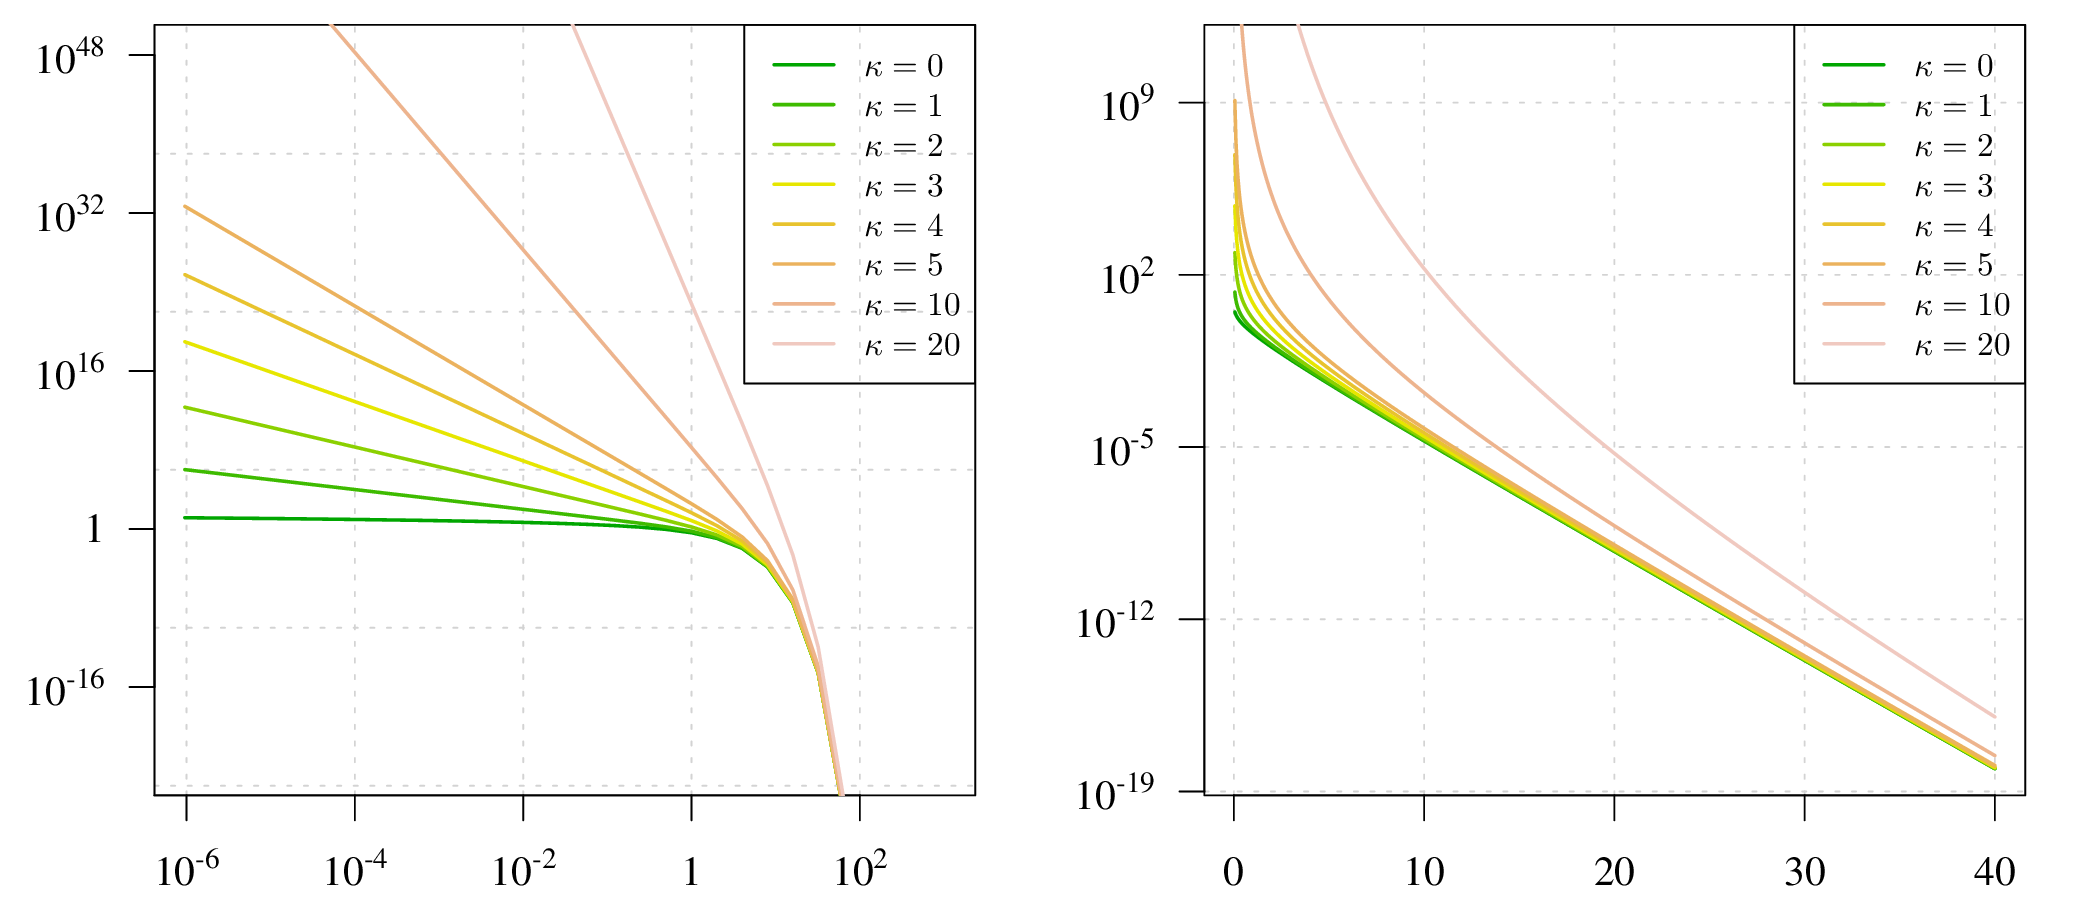
\includegraphics[width=0.7\linewidth]{figures/bessel} 

}

\caption{在 \(\kappa\)
取不同值时的贝塞尔函数图像:横轴表示距离\(u\),纵轴表示函数值\(\mathcal{K}_{\kappa}(u)\)}\label{fig:bessel-function}
\end{figure}




\hypertarget{sec:Laplace-approximation}{%
\section{拉普拉斯近似}\label{sec:Laplace-approximation}}

先回顾一下基本的泰勒展开,将一个函数 \(f(x)\) 在点 \(a\)
处展开成和的形式,有时候是无穷多项,可以使用其中的有限项作为近似,通常会选用前三项,即到达函数
\(f(x)\) 二阶导的位置。
\[ f(x) = f(a) + \frac{f'(a)}{1!}(x-a) + \frac{f''(a)}{2!}(x-a)^2 + \frac{f'''(a)}{3!}(x-a)^3 + \ldots \]
\noindent 以基本的抛物线函数 \(f(x) = x^2\) 为例,考虑将它在 \(a = 2\)
处展开。首先计算 \(f(x)\) 的各阶导数
\[ f(x) = x^2, \quad f'(x) = 2x, \quad f''(x) = 2, \quad f^{(n)}(x) = 0, \quad n = 3,4,\ldots \]
\noindent 因此,\(f(x)\) 可以展开成有限项的和的形式
\[ f(x) = x^2 = 2^2 + 2(2)(x-2) + \frac{2}{2}(x-2)^2 \]
拉普拉斯近似本质上是用正态分布来近似任意分布
\(g(x)\),用泰勒展开的前三项近似 \(\log g(x)\),展开的位置是密度函数
\(g(x)\) 的极值点 \(\hat{x}\),则有
\[ \log g(x) \approx \log g(\hat{x}) + \frac{\partial \log g(\hat{x})}{\partial x} (x - \hat{x}) + \frac{\partial^2 \log g(\hat{x})}{2\partial x^2} (x - \hat{x})^2 \]
\noindent 由于是在函数 \(g(x)\) 的极值点 \(\hat{x}\) 展开, 所以
\(x = \hat{x}\) 一阶导是 0,用曲率去估计方差是
\(\hat{\sigma}^2 = -1/\frac{\partial^2 \log g(\hat{x})}{2\partial x^2}\),再重写上述近似
\[ \log g(x) \approx \log g(\hat{x}) - \frac{1}{2\hat{\sigma}^2} (x - \hat{x})^2 \]
\noindent 现在,用这个结果做正态近似,将上式两端先取指数,再积分,移去常数项
\[ \int g(x) \mathrm{d}x = \int \exp[\log g(x)] \mathrm{d}x \approx \mathrm{constant} \int \exp[- \frac{(x - \hat{x})^2}{2\hat{\sigma}^2}] \mathrm{d}x \]
\noindent 则拉普拉斯方法近似任意密度函数 \(g(x)\) 得到的正态分布的均值为
\(\hat{x}\), \(\hat{x}\) 可以通过求解方程 \(g'(x) = 0\) 获得,方差为
\(\hat{\sigma}^2 = -1/g''(\hat{x})\)。下面以卡方分布 \(\chi^2\)
为例,由于 \begin{align*}
    f(x; k) & = \frac{ x^{k/2-1} \mathrm{e}^{-x/2} }{ 2^{k/2}\Gamma(k/2) }, x \geq 0 \quad \log f(x) = (k/2 - 1) \log x - x/2 \\
 \log f'(x) & = (k/2-1)/x - 1/2 = 0 \quad \log f''(x)  = -(k/2-1)/x^2
\end{align*} \noindent 所以,卡方分布的拉普拉斯近似为
\[ \chi_{k}^2 \overset{LA}{\sim}  N(\hat{x} = k-2, \hat{\sigma}^2 = 2(k-2)) \]
\noindent 自由度越大,近似效果越好,对于多元分布的情况不难推广,使用多元泰勒展开和黑塞矩阵即可表示\citep{Tierney1986}。

\hypertarget{sec:bayes-prior}{%
\section{先验和后验分布}\label{sec:bayes-prior}}

贝叶斯推断中,常涉及模型参数的先验、后验分布,以及一种特殊的无信息先验分布
--- Jeffreys 先验,下面分别给出它们的概念定义\citep{mao2006}。

\BeginKnitrBlock{definition}[先验分布]
\protect\hypertarget{def:prior-distribution}{}{\label{def:prior-distribution}
\iffalse (先验分布) \fi{} }参数空间 \(\Theta\)
上的任一概率分布都称作先验分布 (prior distribution)。
\EndKnitrBlock{definition}

\BeginKnitrBlock{definition}[后验分布]
\protect\hypertarget{def:posterior-distribution}{}{\label{def:posterior-distribution}
\iffalse (后验分布) \fi{} }在获得样本 \(\mathbf{Y}\) 后,模型参数
\(\boldsymbol{\theta}\) 的后验分布 (posterior distribution) 就是在给定
\(\mathbf{Y}\) 条件下 \(\boldsymbol{\theta}\)
的条件分布。根据条件概率定义、链式法则、全概率公式,有 \begin{align}
\begin{array}{rcll}
p(\boldsymbol{\theta}|\mathbf{Y})  & =  & \displaystyle \frac{p(\boldsymbol{\theta},\mathbf{Y})}{p(\mathbf{Y})}
& \mbox{ [条件概率定义]}
\\[16pt]
& = & \displaystyle \frac{p(\mathbf{Y}|\boldsymbol{\theta}) p(\boldsymbol{\theta})}{p(\mathbf{Y})}
& \mbox{ [链式法则]}
\\[16pt]
& = & \displaystyle \frac{p(\mathbf{Y}|\boldsymbol{\theta})p(\boldsymbol{\theta})}{\int_{\Theta}p(\mathbf{Y},\boldsymbol{\theta})d\boldsymbol{\theta}}
& \mbox{ [全概率公式]}
\\[16pt]
& = & \displaystyle \frac{p(\mathbf{Y}|\boldsymbol{\theta})p(\boldsymbol{\theta})}{\int_{\Theta}p(\mathbf{Y}|\boldsymbol{\theta})p(\boldsymbol{\theta})d\boldsymbol{\theta}}
& \mbox{ [链式法则]}
\\[16pt]
& \propto & \displaystyle p(\mathbf{Y}|\boldsymbol{\theta})p(\boldsymbol{\theta})
& \mbox{ [$\mathbf{Y}$ 已知]}
\end{array} \label{eq:bayes-theorem}
\end{align}
\EndKnitrBlock{definition}

\BeginKnitrBlock{definition}[Jeffreys 先验分布]
\protect\hypertarget{def:Jeffreys-prior-distribution}{}{\label{def:Jeffreys-prior-distribution}
\iffalse (Jeffreys 先验分布) \fi{} }设 \(\mathbf{x} = (x_1,\ldots,x_n)\)
是来自密度函数 \(p(x|\boldsymbol{\theta})\) 的一个样本,其中
\(\boldsymbol{\theta} = (\theta_1,\ldots,\theta_p)\) 是 \(p\)
维参数向量。在对 \(\boldsymbol{\theta}\) 无任何先验信息可用时, Jeffreys
(1961年)利用变换群和 Harr 测度导出 \(\boldsymbol{\theta}\)
的无信息先验分布可用 Fisher
信息阵的行列式的平方根表示。这种无信息先验分布常称为 Jeffreys
先验分布。其求取步骤如下:
\EndKnitrBlock{definition}

\begin{enumerate}
\def\labelenumi{\arabic{enumi}.}
\tightlist
\item
  写出样本的对数似然函数
  \(l(\boldsymbol{\theta}|x) = \sum_{i=1}^{n}\ln p(x_i | \boldsymbol{\theta})\);
\item
  算出参数 \(\boldsymbol{\theta}\) 的 Fisher 信息阵
  \[\mathbf{I}(\boldsymbol{\theta}) = \mathsf{E}_{x|\theta} \big( - \frac{\partial^2 l}{\partial \theta_i \partial \theta_j} \big)_{i,j=1,\ldots,p}\]
  在单参数场合,
  \(\mathbf{I}(\theta) = \mathsf{E}_{x|\theta} \big( - \frac{\partial^2 l}{\partial \theta^2} \big)\);
\item
  \(\boldsymbol{\theta}\) 的无信息先验密度函数为
  \(\pi(\boldsymbol{\theta}) = [\det \mathbf{I}(\theta) ]^{1/2}\),在单参数场合,
  \(\pi(\boldsymbol{\theta}) = [\mathbf{I}(\theta) ]^{1/2}\)。
\end{enumerate}

\hypertarget{bayes-estimates}{%
\section{常用贝叶斯估计}\label{bayes-estimates}}

\BeginKnitrBlock{theorem}[平方损失]
\protect\hypertarget{thm:bayes-estimate-square}{}{\label{thm:bayes-estimate-square}
\iffalse (平方损失) \fi{} }在给定先验分布 \(\pi(\boldsymbol{\theta})\)
和平方损失
\(L(\boldsymbol{\theta},\boldsymbol{\delta}) = (\boldsymbol{\delta} - \boldsymbol{\theta})^2\)
下,\(\boldsymbol{\theta}\) 的贝叶斯估计
\(\boldsymbol{\delta}^{\pi}(x)\) 为后验分布
\(\pi(\boldsymbol{\theta}|x)\) 的均值,即
\(\boldsymbol{\delta}^{\pi}(x) = \mathsf{E}(\boldsymbol{\theta}|x)\)。
\EndKnitrBlock{theorem}

\BeginKnitrBlock{theorem}[0 - 1 损失]
\protect\hypertarget{thm:bayes-estimate-01}{}{\label{thm:bayes-estimate-01}
\iffalse (0 - 1 损失) \fi{} }在给定先验分布 \(\pi(\boldsymbol{\theta})\)
和 \(0\) - \(1\) 损失函数

\begin{equation*}
L(\boldsymbol{\theta},\boldsymbol{\delta}) = 
\begin{cases}
1, & | \boldsymbol{\delta} - \boldsymbol{\theta}| \leq \epsilon \\
0, & | \boldsymbol{\delta} - \boldsymbol{\theta}| > \epsilon
\end{cases}
\end{equation*}

当 \(\epsilon\) 较小时,\(\boldsymbol{\theta}\)
的贝叶斯估计\(\boldsymbol{\delta}^{\pi}(x)\)为后验分布
\(\pi(\boldsymbol{\theta}|x)\) 的众数。
\EndKnitrBlock{theorem}

\BeginKnitrBlock{theorem}[绝对值损失]
\protect\hypertarget{thm:bayes-estimate-abs}{}{\label{thm:bayes-estimate-abs}
\iffalse (绝对值损失) \fi{} }在给定先验分布 \(\pi(\boldsymbol{\theta})\)
和绝对损失函数
\(L(\boldsymbol{\theta},\boldsymbol{\delta}) = |\boldsymbol{\delta} - \boldsymbol{\theta}|\)
下,\(\boldsymbol{\theta}\) 的贝叶斯估计
\(\boldsymbol{\delta}^{\pi}(x)\) 为后验分布
\(\pi(\boldsymbol{\theta}|x)\) 的中位数。
\EndKnitrBlock{theorem}

评价贝叶斯估计 \(\boldsymbol{\delta}^{\pi}(x)\) 的精度常用后验均方误差
\[\mathsf{MSE}(\boldsymbol{\delta}^{\pi}|x) = \mathsf{E}_{\boldsymbol{\theta}|x}(\boldsymbol{\delta}^{\pi} - \boldsymbol{\theta})^2\]
表示,或用其平方根\([\mathsf{MSE}(\boldsymbol{\delta}^{\pi}|x)]^{1/2}\)
(称为标准误)表示。容易算得
\[\mathsf{MSE}(\boldsymbol{\delta}^{\pi}|x) = \mathsf{Var}(\boldsymbol{\delta}^{\pi}|x) + [\boldsymbol{\delta}^{\pi}(x) - \mathsf{E}(\boldsymbol{\theta}|x)]^2\]
可见,当贝叶斯估计\(\boldsymbol{\delta}^{\pi}(x)\)为后验均值时,贝叶斯估计的精度就用\(\boldsymbol{\delta}^{\pi}\)的后验方差\(\mathsf{Var}(\boldsymbol{\delta}^{\pi}|x)\)
表示,或用后验标准差
\([\mathsf{Var}(\boldsymbol{\delta}^{\pi}|x)]^{1/2}\) 表示
\citep{mao2006}。

\hypertarget{Curse-of-Dimensionality}{%
\section{蒙特卡罗积分}\label{Curse-of-Dimensionality}}

一般地,空间广义线性混合效应模型的统计推断总是不可避免的要面对高维积分,处理高维积分的方法一个是寻找近似方法避免求积分,一个是寻找有效的随机模拟方法直接求积分。这里,介绍蒙特卡罗方法求积分,以计算
\(N\) 维超立方体的内切球的体积为例说明。

假设我们有一个 \(N\) 维超立方体,其中心在坐标
\(\mathbf{0} = (0,\ldots,0)\)。超立方体在点
\((\pm 1/2,\ldots,\pm 1/2)\),有 \(2^{N}\)
个角落,超立方体边长是1,\(1^{N}=1\),所以它的体积是1。如果
\(N=1\),超立方体是一条从 \(-\frac{1}{2}\) 到 \(\frac{1}{2}\)
的单位长度的线,如果 \(N=2\),超立方体是一个单位正方形,对角是
\(\left( -\frac{1}{2}, -\frac{1}{2} \right)\) 和
\(\left( \frac{1}{2}, \frac{1}{2} \right)\),如果
\(N=3\),超立方体就是单位体积的立方体,对角是
\(\left( -\frac{1}{2}, -\frac{1}{2}, -\frac{1}{2} \right)\) 和
\(\left( \frac{1}{2}, \frac{1}{2}, \frac{1}{2} \right)\),依此类推,\(N\)
维超立方体体积是1,对角是
\(\left( -\frac{1}{2}, \ldots, -\frac{1}{2} \right)\) 和
\(\left( \frac{1}{2}, \ldots, \frac{1}{2} \right)\)。

现在,考虑 \(N\) 维超立方体的内切球,我们把它称为 \(N\)
维超球,它的中心在原点,半径是 \(\frac{1}{2}\)。我们说点 \(y\)
在超球内,意味着它到原点的距离小于半径,即
\(\| y \| < \frac{1}{2}\)。一维情形下,超球是从的线,包含了整个超立方体。二维情形下,超球是中心在原点,半径为
\(\frac{1}{2}\)
的圆。三维情形下,超球是立方体的内切球。已知单位超立方体的体积是1,但是其内的内切球的体积是多少呢?我们已经学过如何去定义一个积分计算半径为
\(r\) 的二维球(即圆)的体积(即面积)是
\(\pi r^2\),三维情形下,内切球是
\(\frac{4}{3}\pi r^3\)。但是更高维的欧式空间里,内切球的体积是多少呢?

在这种简单的体积积分设置下,当然可以去计算越来越复杂的多重积分,但是这里介绍采样的方法去计算积分,即所谓的蒙特卡罗方法,由梅特罗波利斯,冯\(\cdot\)诺依曼和乌拉姆等在美国核武器研究实验室创立,当时正值二战期间,为了研制原子弹,出于保密的需要,与随机模拟相关的技术就代号蒙特卡罗。现在,蒙特卡罗方法占据现代统计计算的核心地位,特别是与贝叶斯相关的领域。

用蒙特卡罗方法去计算单位超立方体内的超球,首先需要在单位超立方体内产生随机点,然后计算落在超球内的点的比例,即超球的体积。随着点的数目增加,估计的体积会收敛到真实的体积。因为这些点都独立同均匀分布,根据中心极限定理,误差下降的比率是
\(\mathcal{O}\left( 1 / \sqrt{n} \right)\),这也意味着每增加一个小数点的准确度,样本量要增加
100 倍。

\begin{longtable}[]{@{}lcccccccccc@{}}
\caption{\label{tab:calculate-volume-of-hyperball} 前 10
维单位超立方体内切球的体积,超立方体内随机模拟的点的个数是
100000(已经四舍五入保留小数点后三位)}\tabularnewline
\toprule
维数 & 1 & 2 & 3 & 4 & 5 & 6 & 7 & 8 & 9 & 10\tabularnewline
\midrule
\endfirsthead
\toprule
维数 & 1 & 2 & 3 & 4 & 5 & 6 & 7 & 8 & 9 & 10\tabularnewline
\midrule
\endhead
体积 & 1.000 & 0.784 & 0.525 & 0.307 & 0.166 & 0.081 & 0.037 & 0.016 &
0.006 & 0.0027\tabularnewline
\bottomrule
\end{longtable}

表 \ref{tab:calculate-volume-of-hyperball} 列出了前 10
维超球的体积,从上述计算过程中,我们发现随着维数增加,超球的体积迅速变小。这里有一个反直观的现象,内切球的体积竟然随着维数的增加变小,并且在
10 维的情形下,内切球的体积已不到超立方体的
0.3\%,可以预见如果这个积分是 100
维甚至更多,那么内切球相比于正方体仅仅是一个极小的角落,随机点会越来越难以落在内切球内。甚至会因为所需要的随机数太多或者计算机资源的限制,而不可计算,开发更加高效的随机模拟算法也就势在必行。

\hypertarget{sec:stan-samplers}{%
\section{Stan 简介}\label{sec:stan-samplers}}

在上世纪 40\textasciitilde{}50
年代,由梅特罗波利斯,冯\(\cdot\)诺依曼和乌拉姆 (Stanislaw Ulam)
创立蒙特卡罗方法,为了纪念乌拉姆,Stan 就以他的名字命名。Stan 是一门基于
C++
的概率编程语言,主要用于贝叶斯推断,它的代码完全\href{http://mc-stan.org/}{开源}的,托管在
\href{https://github.com/stan-dev/stan}{Github} 上,自 2012 年 8 月 30
日发布第一个 1.0 版本以来,截至写作时间已发布 33 个版本,目前最新版本是
2.18.0。使用 Stan,用户需提供数据、Stan 代码写的脚本模型,编译 Stan
写的程序,然后与数据一起运行,模型参数的后验模拟过程是自动实现的。除了可以在命令行环境下编译运行
Stan 脚本中写模型外,Stan 还提供其他编程语言的接口,如
R、Python、Matlab、Mathematica、Julia
等等,这使得熟悉其他编程语言的用户可以方便地调用和分析数据。但是,与
Python、R等 这类解释型编程语言不同, Stan 代码需要先翻译成 C++
代码,然后使用系统编译器 (如 GCC) 编译,若使用 R
语言接口,编译后的动态链接库可以载入 R 内存中,再被其他 R 函数调用执行。

随机模拟的前提是有能产生高质量高效的伪随机数发生器,只有周期长,生成速度快,能通过一系列统计检验的伪随机数才能用作统计模拟,Stan
内置了 Mersenne-Twister 发生器,它的周期长达
\(2^{19937}-1\),通过了一系列严格的检验,被广泛采用到现代软件中,如
Octave 和 Matlab 等 \citep{Huang2017COS}。除了 Mersenne Twister
随机数发生器,Stan 还使用了 \href{https://www.boost.org/}{Boost C++} 和
\href{http://eigen.tuxfamily.org/index.php?title=Main_Page}{Eigen C++}
等模版库用于线性代数计算,这样的底层设计路线使得 Stan 的运算效率很高。

Stan 内置的采样器 No-U-Turn (简称 NUTS) 源于汉密尔顿蒙特卡罗算法
(Hamiltonian Monte Carlo,简称 HMC),最早由 Hoffman 和 Gelman
(2014年) \citep{hoffman2014} 提出。与 Stan 有相似功能的软件 BUGS 和
JAGS 主要采用的是 Gibbs 采样器,前者基于 Pascal 语言开发于 1989 年至
2004 年,后者基于 C++ 活跃开发于 2007 年至 2013 年。在时间上, Stan
具有后发优势,特别在灵活性和扩展性方面,它支持任意的目标函数,模型语言也更加简单易于推广学习,其每一行都是命令式的语句,而
BUGS 和 JAGS 采用声明式;在大量数据的建模分析中, Stan
可以更快地处理复杂模型,这一部分归功于它高效的算法实现和内存管理,另一部分在于高级的
MCMC 算法 --- 带 NUTS 采样器的 HMC 算法。

Rubin (1981年) \citep{Rubin1981} 分析了 Alderman 和 Powers
\citep{Alderman1980} 收集的原始数据,得出表
\ref{tab:eight-high-schools}, Gelman 和 Carlin 等 (2003年)
\citep{Gelman2003} 建立分层正态模型 \eqref{eq:hierarchical-normal-models}
分析 Eight Schools
数据集,由美国教育考试服务调查搜集,用以分析不同的培训项目对学生考试分数的影响,其随机调查了
8 所高中,学生的成绩作为培训效应的估计 \(y_j\),其样本方差
\(\sigma^2_j\),数据集见表
\ref{tab:eight-high-schools}。这里再次以该数据集和模型为例介绍 Stan
的使用。

\begin{longtable}[]{@{}ccccccccc@{}}
\caption{\label{tab:eight-high-schools} Eight Schools 数据集}\tabularnewline
\toprule
School & A & B & C & D & E & F & G & H\tabularnewline
\midrule
\endfirsthead
\toprule
School & A & B & C & D & E & F & G & H\tabularnewline
\midrule
\endhead
\(y_i\) & 28 & 8 & -3 & 7 & -1 & 1 & 18 & 12\tabularnewline
\(\sigma_i\) & 15 & 10 & 16 & 11 & 9 & 11 & 10 & 18\tabularnewline
\bottomrule
\end{longtable}

\begin{equation}
\begin{aligned}
     \mu & \sim \mathcal{N}(0,5) \\
    \tau & \sim \text{Half-Cauchy}(0,5) \\
p(\mu,\tau) & \propto 1 \\
  \eta_i & \sim \mathcal{N}(0,1) \\
\theta_i &  =   \mu + \tau \cdot \eta_i \\
     y_i & \sim \mathcal{N}(\theta_i,\sigma^2_{i}), i = 1,\ldots,8
\end{aligned}
\label{eq:hierarchical-normal-models}
\end{equation}

根据公式组 \eqref{eq:hierarchical-normal-models}
指定的各参数的先验分布,分层正态模型可以在 Stan
中写成如下形式,我们在工作目录下把它保存为 \texttt{8schools.stan}
,供后续编程使用。

\begin{verbatim}
// saved as 8schools.stan
data {
  int<lower=0> J; // number of schools 
  real y[J]; // estimated treatment effects
  real<lower=0> sigma[J]; // s.e. of effect estimates 
}
parameters {
  real mu; // population mean
  real<lower=0> tau; // population sd
  real eta[J]; // school-level errors
}
transformed parameters {
  real theta[J];  // schools effects
  for (j in 1:J)
    theta[j] = mu + tau * eta[j];
  // theta = mu + tau*eta;
}
model {
  // set prior for mu or uniform prior distribution default
  // target += normal_lpdf(mu  | 0, 10); 
  // target += cauchy_lpdf(tau | 0, 25); # the same as mu
  target += normal_lpdf(eta | 0, 1);
  target += normal_lpdf(y | theta, sigma); // target distribution
  // y ~ normal(theta, sigma);
}
\end{verbatim}

上述 Stan 代码的第一段提供数据:学校的数目 \(J\),估计值
\(y_1,\ldots,y_{J}\),标准差
\(\sigma_1,\ldots,\sigma_{J}\),数据类型可以是整数、实数,结构可以是向量,或更一般的数组,还可以带约束,如在这个模型中
\(J\) 限制为非负, \(\sigma_{J}\) 必须是正的,另外两个反斜杠 //
表示注释。第二段代码声明参数:模型中的待估参数,学校总体的效应
\(\theta_j\),均值 \(\mu\),标准差 \(\tau\),学校水平上的误差 \(\eta\)
和效应 \(\theta\)。在这个模型中,用 \(\mu,\tau,\eta\) 表示 \(\theta\)
而不是直接声明 \(\theta\)
作一个参数,通过这种参数化,采样器的运行效率会提高,还应该尽量使用向量化操作代替
for 循环语句。最后一段是模型:稍微注意的是,正文中正态分布
\(\mathcal{N}(\cdot,\cdot)\) 中后一个位置是方差,而 Stan
代码中使用的是标准差。\texttt{target\ +=\ normal\_lpdf(y\ \textbar{}\ theta,\ sigma)}
和 \texttt{y\ \textasciitilde{}\ normal(theta,\ sigma)}
对模型的贡献是一样的,都使用正态分布的对数概率密度函数,只是后者扔掉了对数后验密度的常数项而已,这对于
Stan 的采样、近似和优化算法没有影响 \citep{Stan2017JSS}。

算法运行的硬件环境是 16 核 32 线程主频 2.8 GHz 英特尔至强 E5-2680
处理器,系统环境 CentOS 7,R 软件版本 3.5.1,RStan 版本
2.17.3。算法参数设置了 4 条迭代链,每条链迭代 10000
次,为复现模型结果随机数种子设为 2018。

分层正态模型\eqref{eq:hierarchical-normal-models} 的参数
\(\mu,\tau\),及其参数化引入的中间参数
\(\eta_i,\theta_i,i=1,\ldots,8\),还有对数后验 \(\mathrm{lp}\_\_\)
的估计值见表 \ref{tab:eight-schools-output}。

\begin{longtable}[]{@{}lrrrrrrrrrr@{}}
\caption{\label{tab:eight-schools-output} 对 Eight Schools
数据集建立分层正态模型 \eqref{eq:hierarchical-normal-models},采用 HMC
算法估计模型各参数值}\tabularnewline
\toprule
& mean & se\_mean & sd & 2.5\% & 25\% & 50\% & 75\% & 97.5\% & n\_eff &
Rhat\tabularnewline
\midrule
\endfirsthead
\toprule
& mean & se\_mean & sd & 2.5\% & 25\% & 50\% & 75\% & 97.5\% & n\_eff &
Rhat\tabularnewline
\midrule
\endhead
\(\mu\) & 7.99 & 0.05 & 5.02 & -1.65 & 4.75 & 7.92 & 11.15 & 18.10 &
8455 & 1\tabularnewline
\(\tau\) & 6.47 & 0.06 & 5.44 & 0.22 & 2.45 & 5.18 & 9.07 & 20.50 & 7375
& 1\tabularnewline
\(\eta_1\) & 0.40 & 0.01 & 0.93 & -1.49 & -0.21 & 0.42 & 1.02 & 2.19 &
16637 & 1\tabularnewline
\(\eta_2\) & 0.00 & 0.01 & 0.87 & -1.73 & -0.58 & 0.00 & 0.57 & 1.70 &
16486 & 1\tabularnewline
\(\eta_3\) & -0.20 & 0.01 & 0.93 & -1.99 & -0.82 & -0.20 & 0.41 & 1.66 &
20000 & 1\tabularnewline
\(\eta_4\) & -0.04 & 0.01 & 0.88 & -1.80 & -0.60 & -0.04 & 0.53 & 1.74 &
20000 & 1\tabularnewline
\(\eta_5\) & -0.36 & 0.01 & 0.88 & -2.06 & -0.94 & -0.38 & 0.20 & 1.42 &
15489 & 1\tabularnewline
\(\eta_6\) & -0.22 & 0.01 & 0.90 & -1.96 & -0.82 & -0.23 & 0.37 & 1.57 &
20000 & 1\tabularnewline
\(\eta_7\) & 0.34 & 0.01 & 0.89 & -1.49 & -0.24 & 0.36 & 0.93 & 2.04 &
16262 & 1\tabularnewline
\(\eta_8\) & 0.05 & 0.01 & 0.94 & -1.81 & -0.57 & 0.06 & 0.69 & 1.91 &
20000 & 1\tabularnewline
\(\theta_1\) & 11.45 & 0.08 & 8.27 & -1.86 & 6.07 & 10.27 & 15.50 &
31.68 & 11788 & 1\tabularnewline
\(\theta_2\) & 7.93 & 0.04 & 6.15 & -4.45 & 3.99 & 7.90 & 11.74 & 20.44
& 20000 & 1\tabularnewline
\(\theta_3\) & 6.17 & 0.06 & 7.67 & -11.17 & 2.07 & 6.74 & 10.89 & 19.94
& 16041 & 1\tabularnewline
\(\theta_4\) & 7.66 & 0.05 & 6.51 & -5.63 & 3.75 & 7.72 & 11.62 & 20.78
& 20000 & 1\tabularnewline
\(\theta_5\) & 5.13 & 0.05 & 6.41 & -9.51 & 1.37 & 5.66 & 9.43 & 16.41 &
20000 & 1\tabularnewline
\(\theta_6\) & 6.14 & 0.05 & 6.66 & -8.63 & 2.35 & 6.58 & 10.40 & 18.47
& 20000 & 1\tabularnewline
\(\theta_7\) & 10.64 & 0.05 & 6.76 & -1.14 & 6.11 & 10.11 & 14.52 &
25.88 & 20000 & 1\tabularnewline
\(\theta_8\) & 8.42 & 0.06 & 7.86 & -7.24 & 3.91 & 8.26 & 12.60 & 25.24
& 16598 & 1\tabularnewline
lp\_\_ & -39.55 & 0.03 & 2.64 & -45.41 & -41.15 & -39.31 & -37.67 &
-35.12 & 6325 & 1\tabularnewline
\bottomrule
\end{longtable}

表 \ref{tab:eight-schools-output} 的列为后验量的估计值:依次是后验均值
\(\mathsf{E}(\mu|Y)\)、 蒙特卡罗标准误(Monte Carlo standard
error)、后验标准差 (standard deviation) \(\mathsf{E}(\sigma|Y)\)
、后验分布的 5 个分位点、有效样本数 \(n_{eff}\) 和潜在尺度缩减因子
(potential scale reduction factor),最后两个量
用来分析采样效率和评估迭代序列的平稳性;最后一行表示每次迭代的未正则的对数后验密度
(unnormalized log-posterior density)
\(\hat{R}\),当链条都收敛到同一平稳分布的时候,\(\hat{R}\) 接近 1。

这里对 \(\tau\) 采用的非信息先验是均匀先验,参数 \(\tau\) 的 95\%
的置信区间是 \((0.22,20.5)\), 数据支持 \(\tau\) 的范围低于 20.5。

\begin{figure}

{\centering 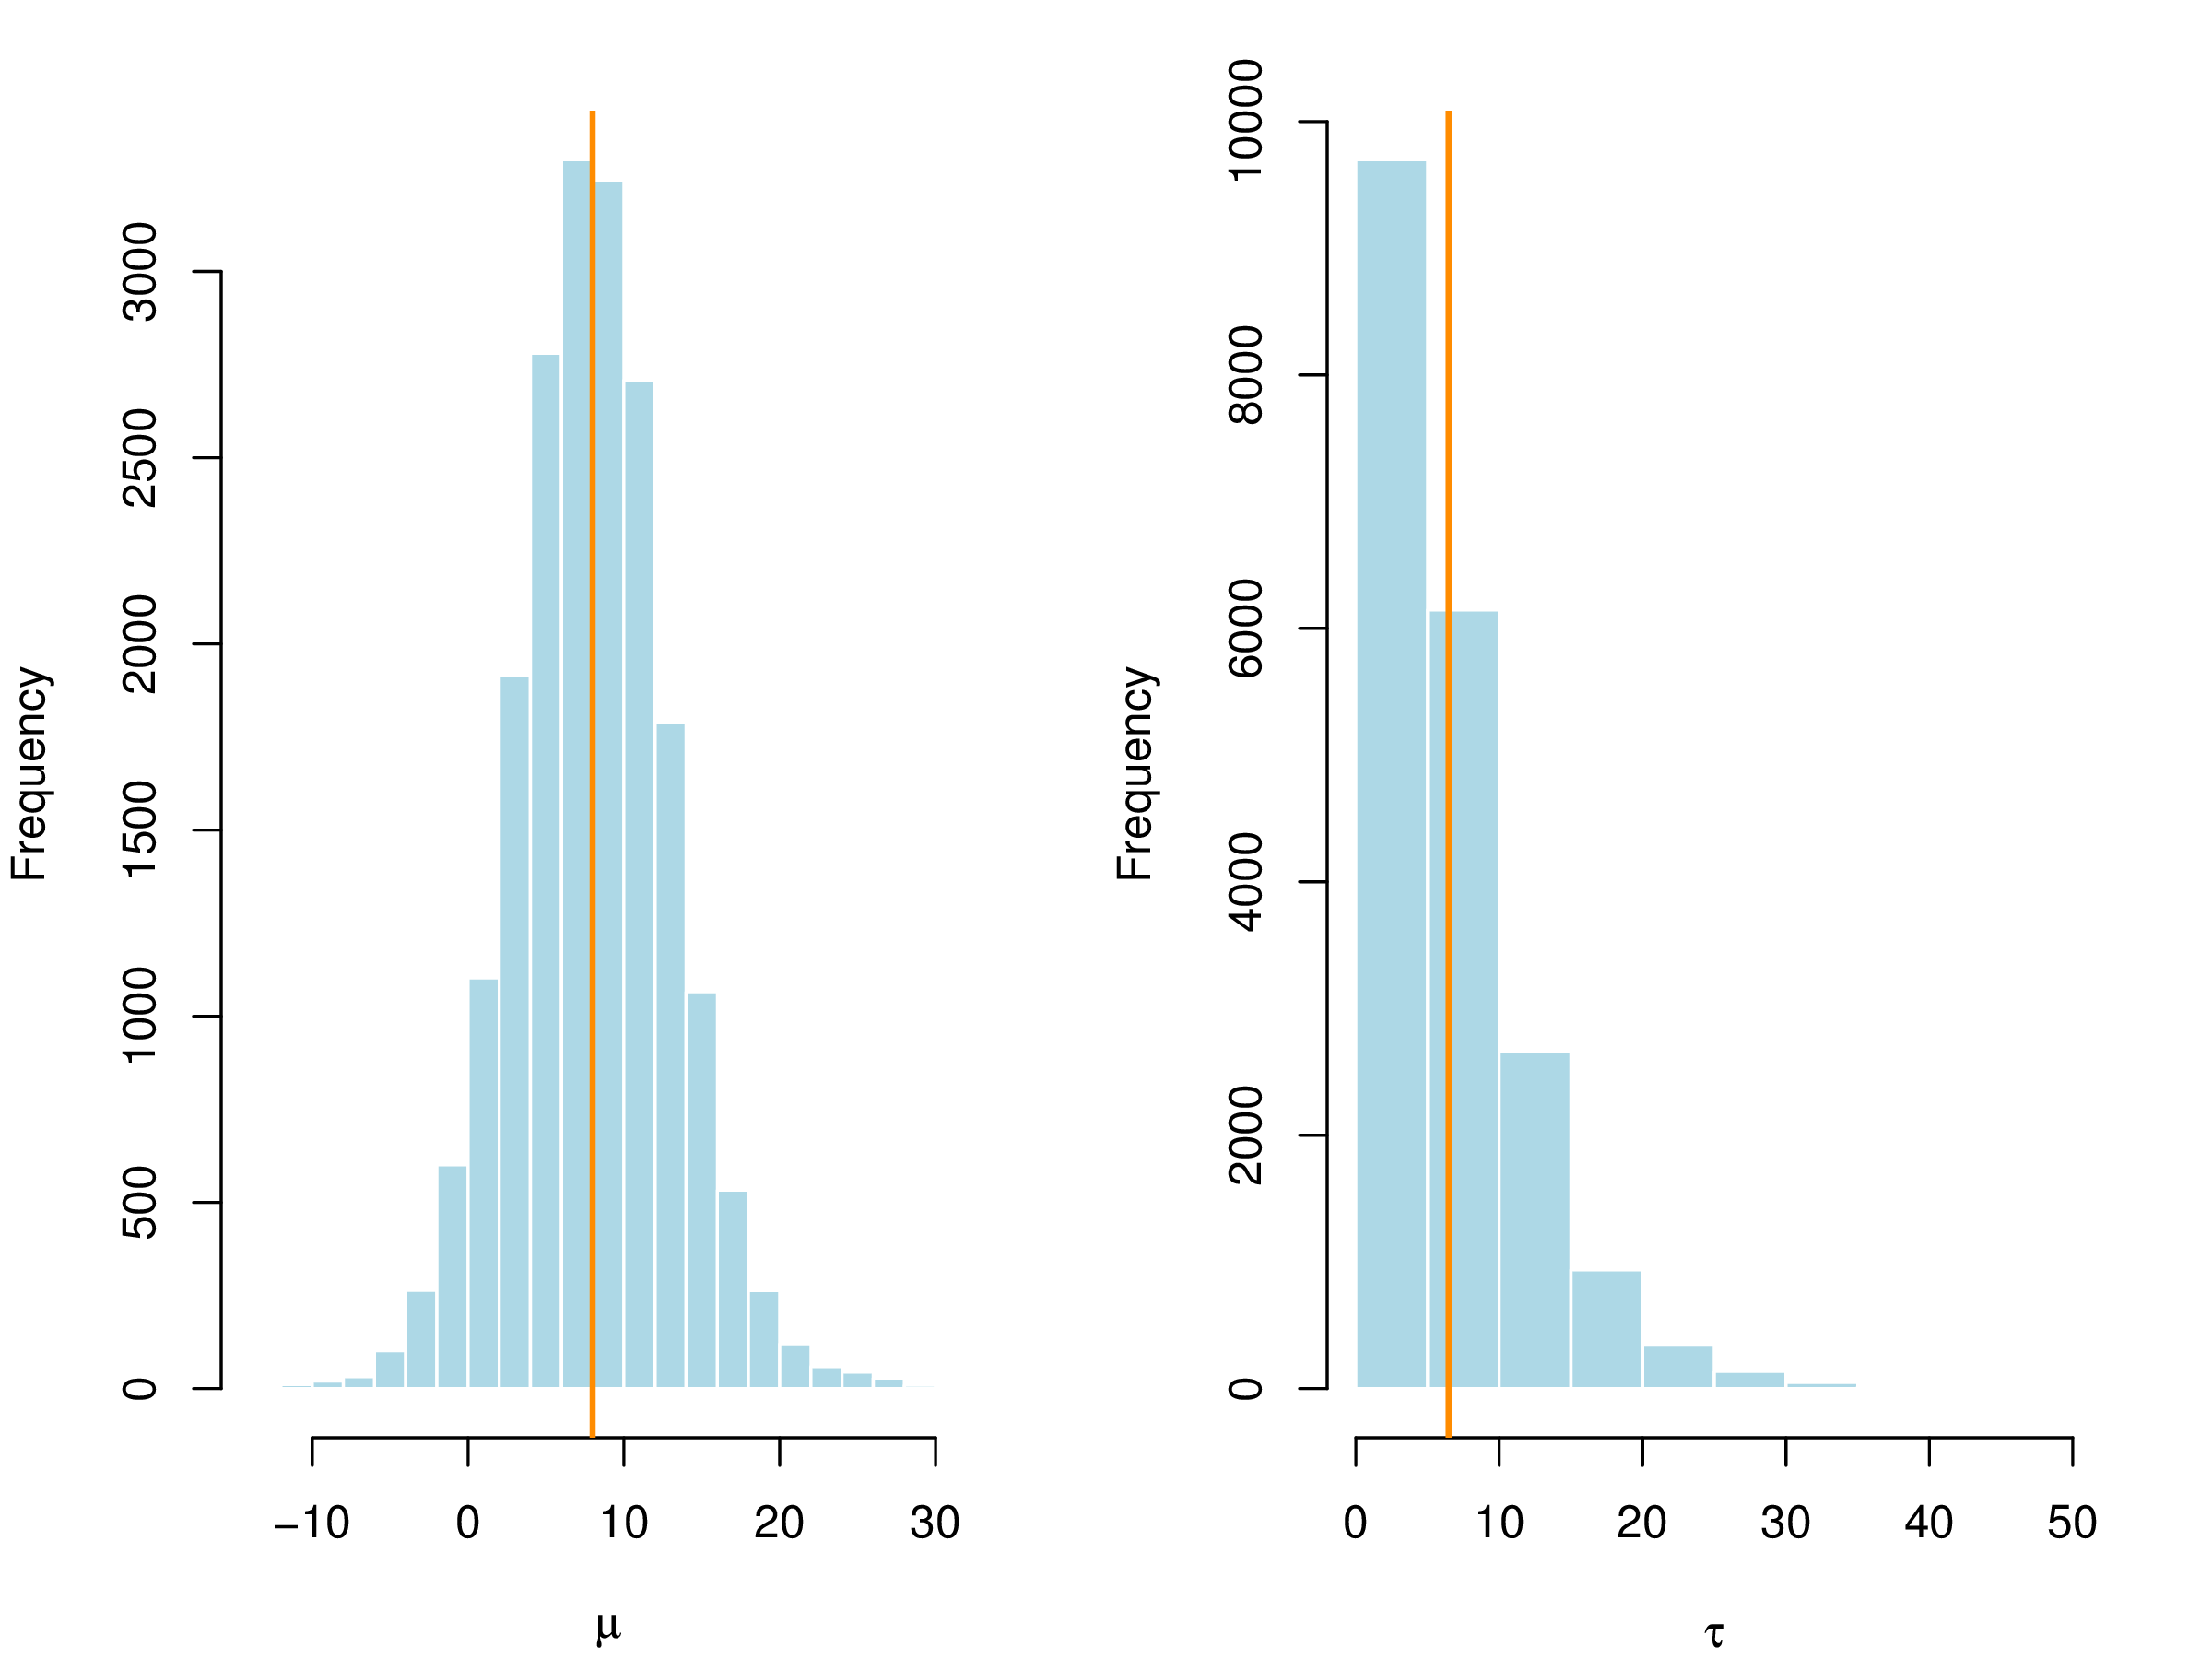
\includegraphics[width=0.7\linewidth]{figures/posterior_mu_tau} 

}

\caption{对 $\mu,\tau$ 给定均匀先验,后验均值 $\mu$ 和标准差 $\tau$ 的直方图}\label{fig:posterior-mu-tau}
\end{figure}

为了得到可靠的后验估计,做出合理的推断,诊断序列的平稳性是必不可少的部分,前
5000 次迭代作为 warm-up 阶段,后 5000 次迭代用作参数的推断,图
\ref{fig:posterior-mu-tau} (a) 给出 \(\mu\) 和 \(\log(\tau)\)
的迭代序列图,其中橘黄色线分别是对应的后验均值(表
\ref{tab:eight-schools-output}的第一列),图 \ref{fig:posterior-mu-tau}
(b) 分别给出 \(\log(\tau)\)
的蒙特卡罗误差,图中显示随着迭代次数增加,蒙特卡罗误差趋于稳定,说明参数
\(\tau\)
的迭代序列达到平稳分布,即迭代点列可以看作来自参数的后验分布的样本。

\begin{figure}[!htb]

{\centering \subfloat[参数 $\log(\tau)$ 和 $\mu$ 的迭代序列图(trace plot)\label{fig:diagnostic1}]{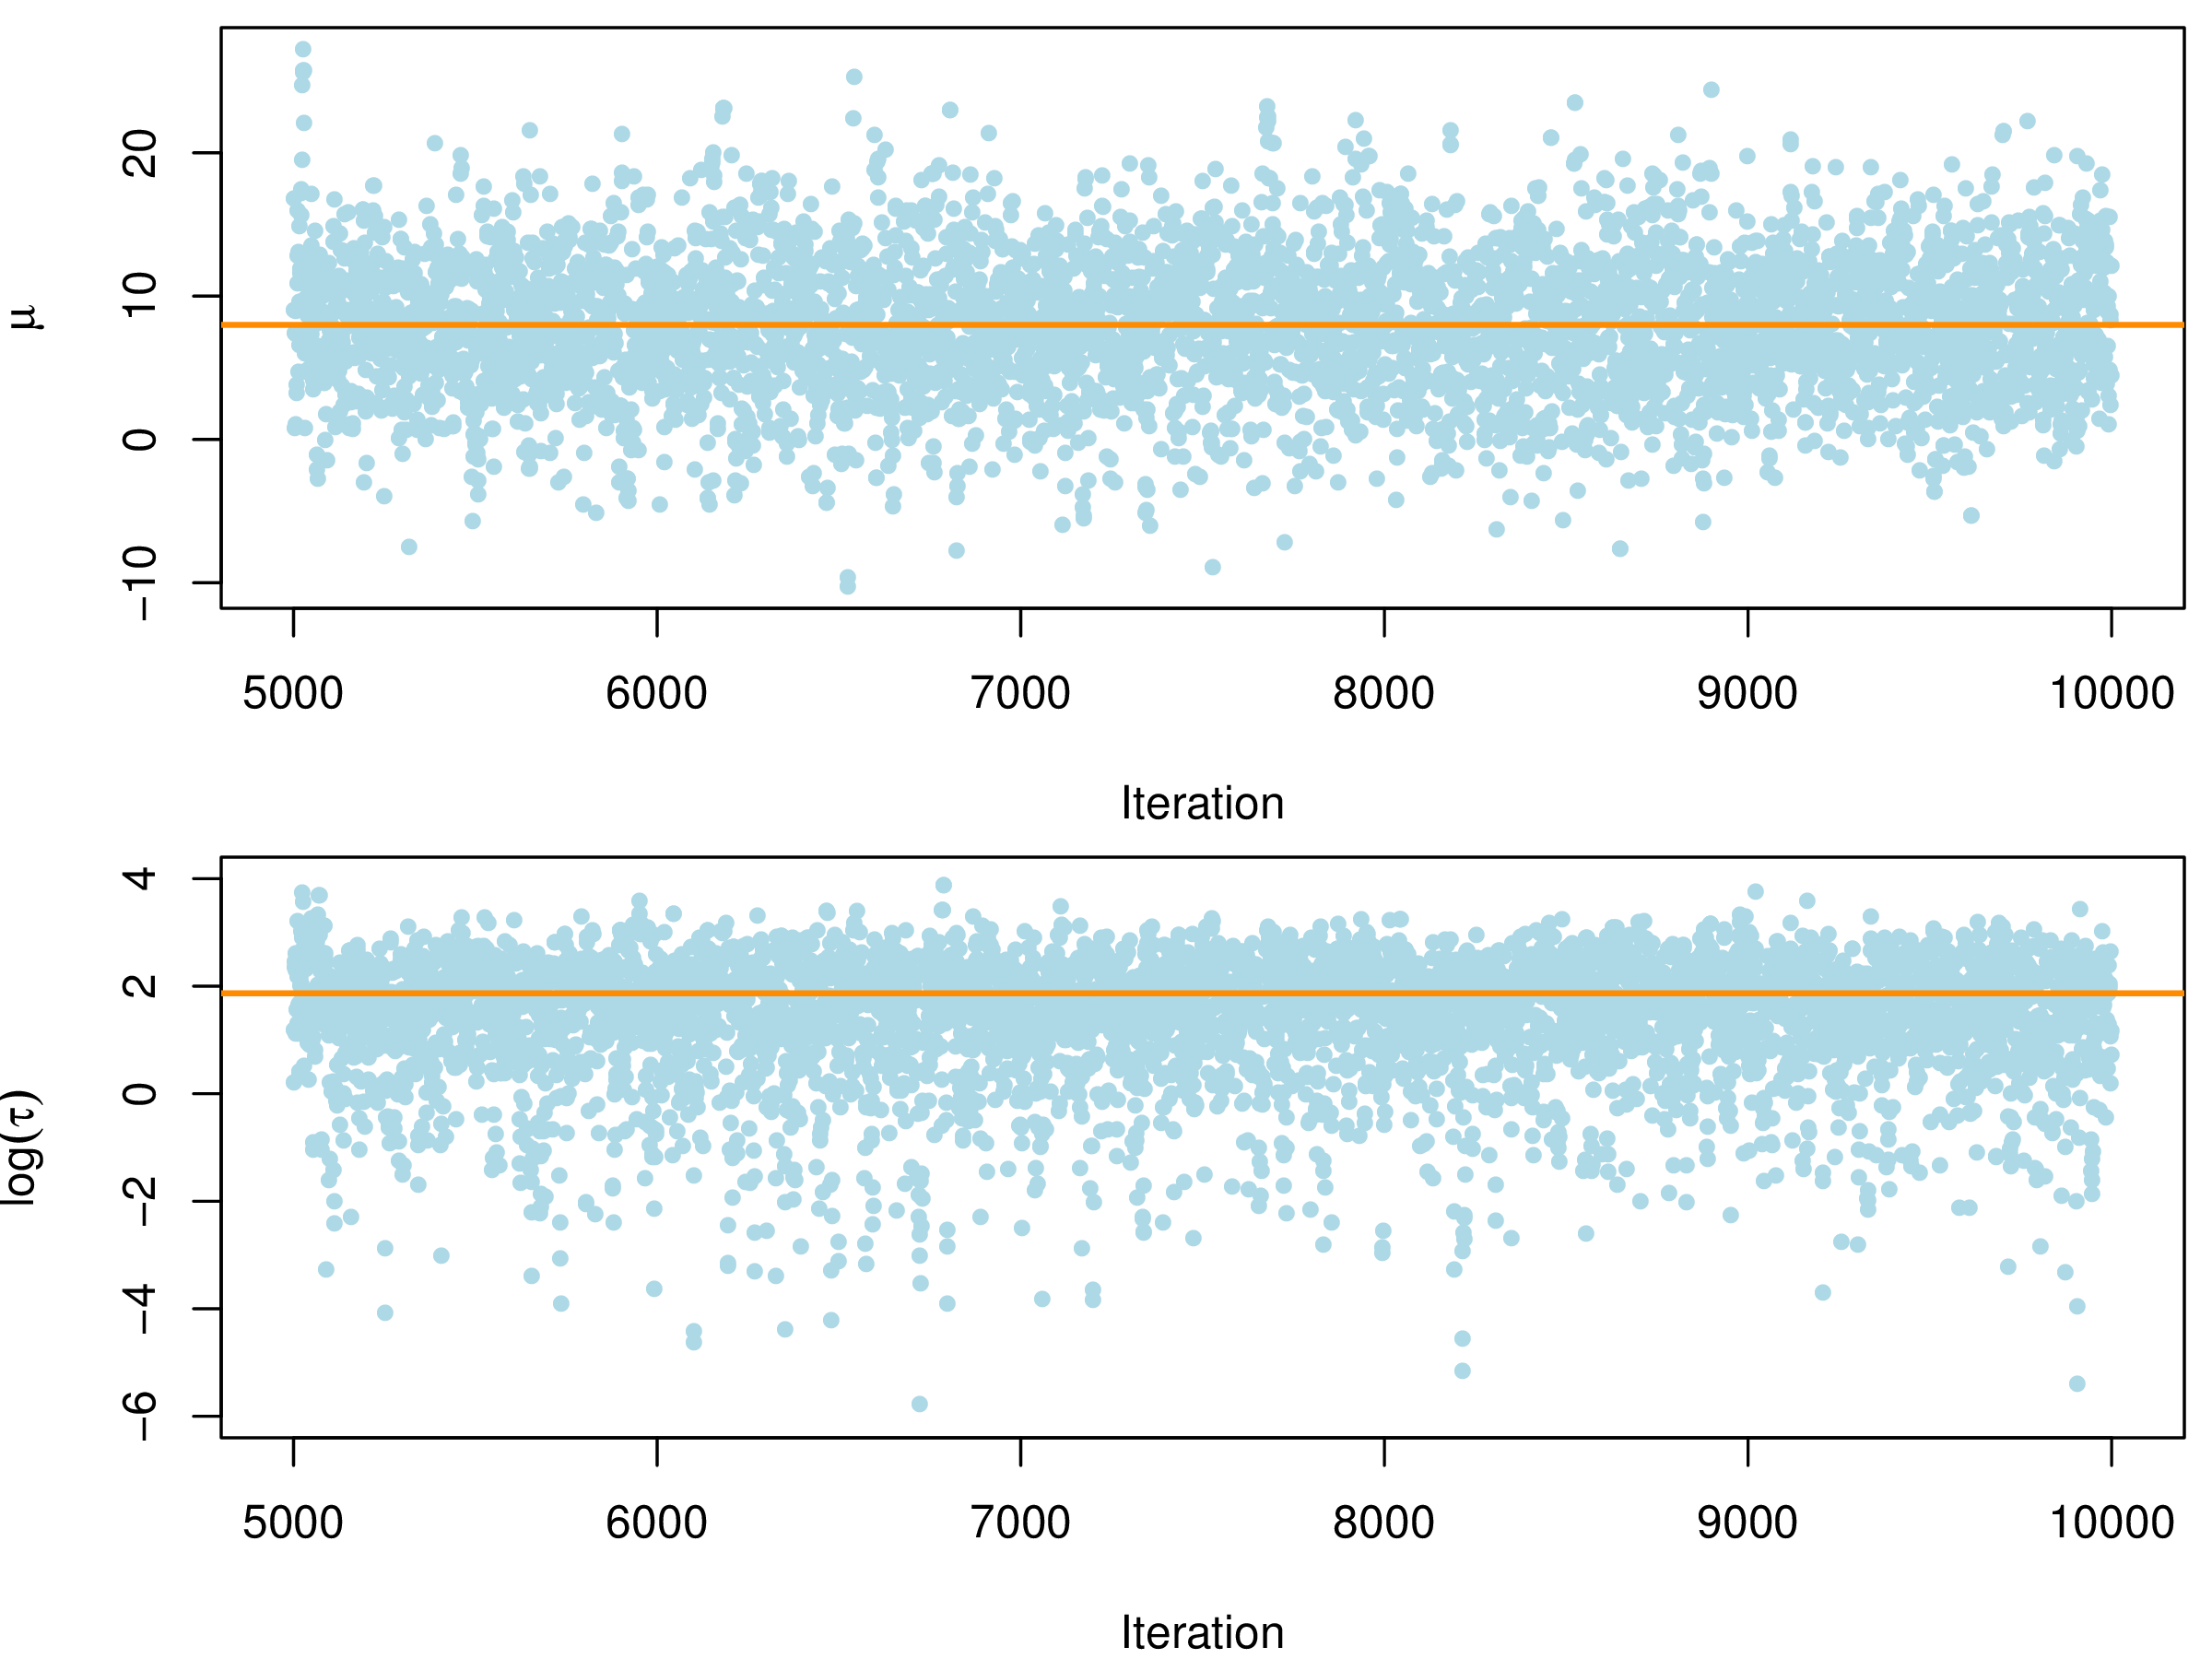
\includegraphics[width=0.7\linewidth]{figures/trace_mu_log_tau} }\\\subfloat[参数 $\log(\tau)$ 的蒙特卡罗均值误差随迭代次数的变化,右图参数 $\log(\tau),\mu$ 的迭代点对的散点图,其中橘黄色点表示使迭代发散的点\label{fig:diagnostic2}]{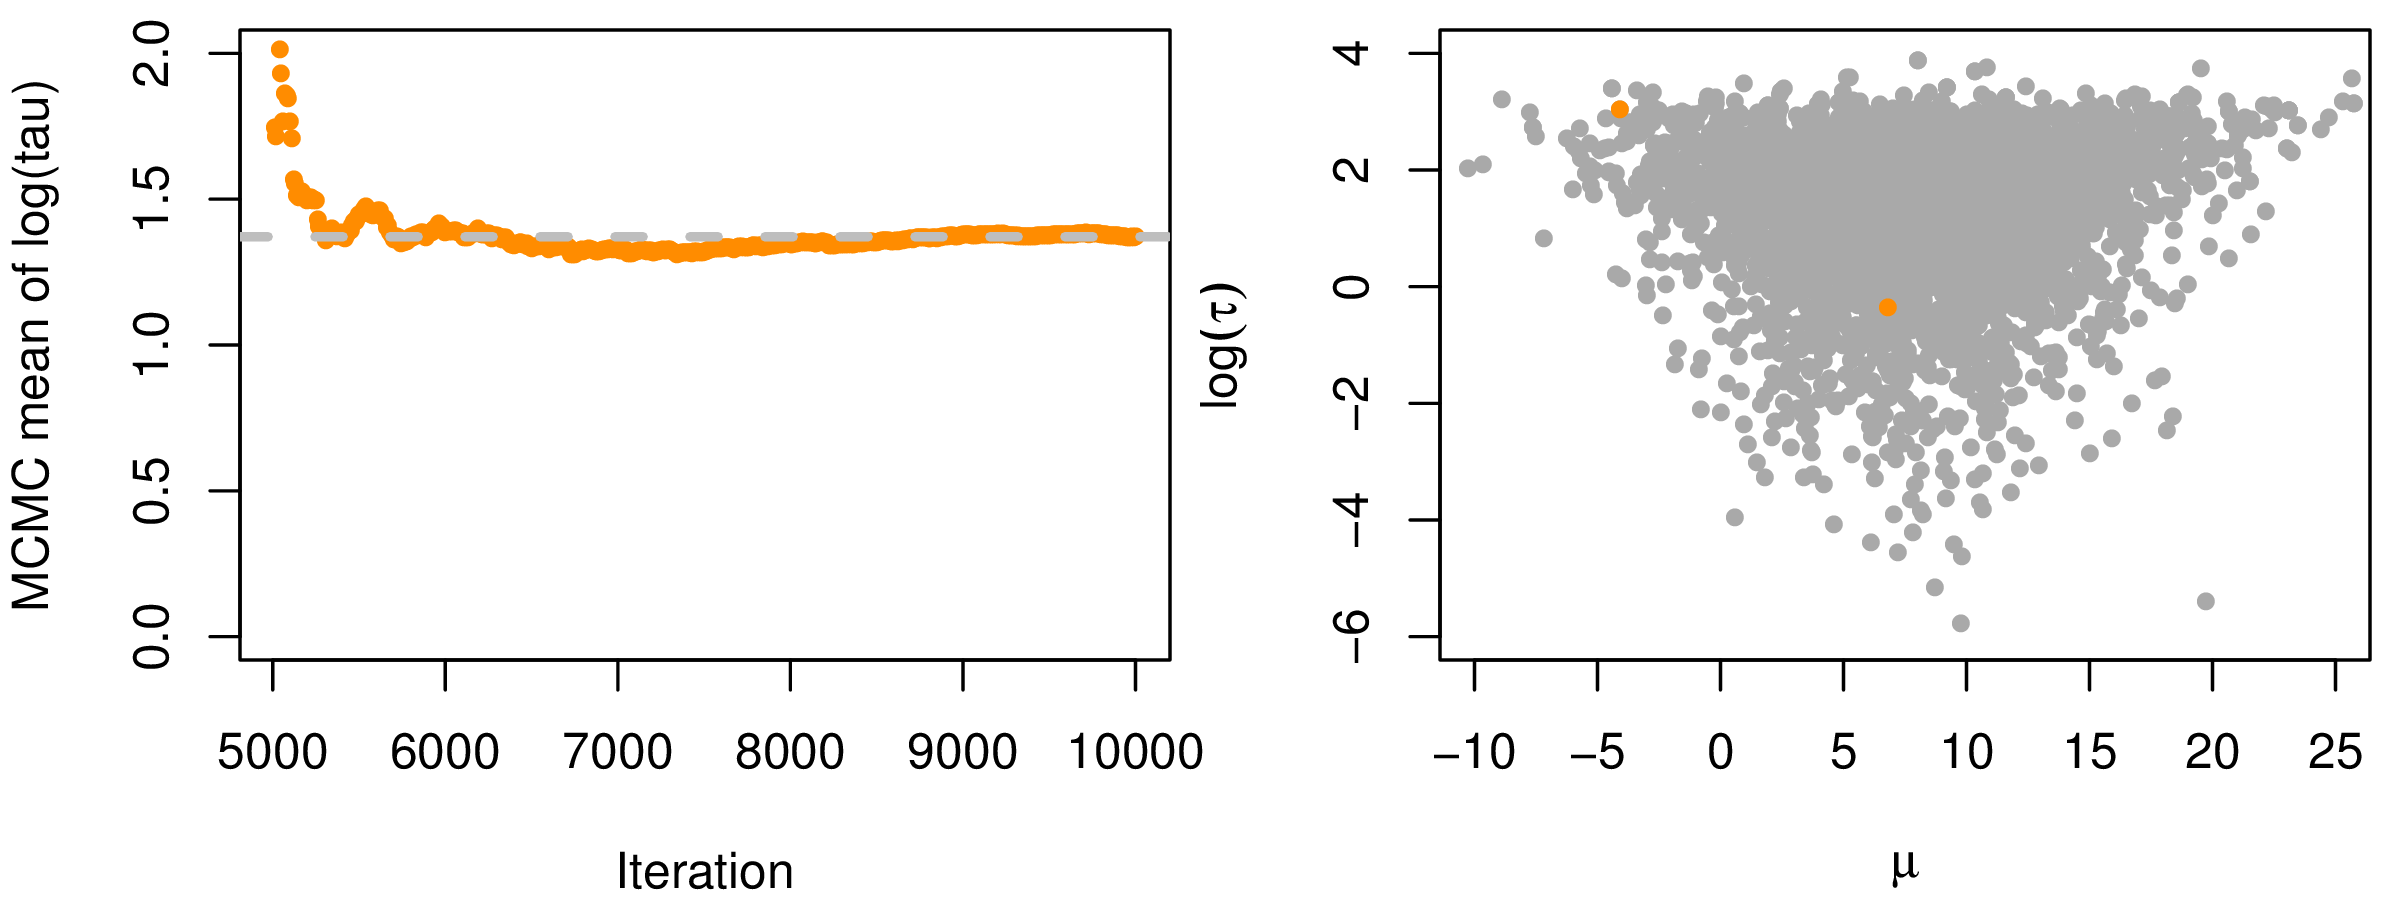
\includegraphics[width=0.7\linewidth]{figures/mcmc_mean_tau_div} }

}

\caption{诊断参数$\mu,\log(\tau)$迭代序列的平稳性}\label{fig:diagnostic}
\end{figure}

为了评估链条之间和内部的混合效果,Gelman 等 \citep{Gelman2013R}
使用潜在尺度缩减因子 (potential scale reduction factor) \(\hat{R}\)
描述链条的波动程度,类似一组数据的方差含义,方差越小波动性越小,数据越集中,这里意味着链条波动性小。一般地,对于每个待估的量
\(\omega\),模拟产生 \(m\) 条链,每条链有 \(n\) 次迭代值
\(\omega_{ij} (i = 1,\ldots,n;j=1,\ldots,m)\),用 \(B\) 和 \(W\)
分别表示链条之间(不妨看作组间方差)和内部的方差(组内方差)

\begin{equation}
\begin{aligned}
& B = \frac{n}{m-1}\sum_{j=1}^{m}(\bar{\omega}_{.j} - \bar{\omega}_{..} ), \quad \bar{\omega}_{.j} = \frac{1}{n}\sum_{i=1}^{n}\omega_{ij}, \quad \bar{\omega}_{..} = \frac{1}{m}\sum_{j=1}^{m} \bar{\omega}_{.j}\\
& W = \frac{1}{m}\sum_{j=1}^{m}s^{2}_{j}, \quad s^{2}_{j} = \frac{1}{n-1}\sum_{i=1}^{n}(\omega_{ij} - \bar{\omega}_{.j})^2
\end{aligned} \label{eq:potential-scale-reduction}
\end{equation}

\noindent \(\omega\) 的后验边际方差 \(\omega|Y\) 是 \(W\) 和 \(B\)
的加权平均

\begin{equation}
\widehat{\mathsf{Var}}^{+}(\omega|Y) = \frac{n-1}{n} W + \frac{1}{n} B 
\end{equation}

当初始分布发散 (overdispersed)
时,这个量会高估边际后验方差,但在链条平稳或 \(n \to \infty\)
时,它是无偏的。同时,对任意有限的 \(n\),组内方差 \(W\) 应该会低估
\(\mathsf{Var}(\omega|Y)\),因为单个链条没有时间覆盖目标分布;在
\(n \to \infty\), \(W\) 的期望会是 \(\mathsf{Var}(\omega|Y)\)。

通过迭代序列采集的样本估计 \(\hat{R}\) 以检测链条的收敛性

\begin{equation}
\hat{R} = \sqrt{\frac{\widehat{\mathsf{Var}}^{+}(\omega|Y)}{W}}
\end{equation}

\noindent 随着 \(n \to \infty\), \(\hat{R}\) 下降到 1。如果 \(\hat{R}\)
比较大,我们有理由认为需要增加模拟次数以改进待估参数 \(\omega\)
的后验分布。从表 \ref{tab:eight-schools-output} 来看,各参数的
\(\hat{R}\) 值都是 1,说明各个迭代链混合得好。

\hypertarget{sec:foundations}{%
\section{本章小结}\label{sec:foundations}}

本章第\ref{sec:exp}节介绍了指数族的一般形式,指出基于样本点的对数似然函数和样本均值、样本方差的关系,以表格的形式列出了正态、泊松和二项分布的各个特征,为第\ref{models}章统计模型和第\ref{algorithms}章参数估计作铺垫。接着,第\ref{sec:lse}节和第\ref{sec:def-mle}节分别介绍了最小二乘估计和极大似然估计的定义、性质,给出了线性模型的最小二乘估计,极大似然估计的相合性和渐进正态性。第\ref{sec:stationary-gaussian-process}节介绍了平稳高斯过程,给出了其均方连续性、可微性定义以及一个均方可微的判断定理,平稳高斯过程作为空间随机效应的实现,多次出现在后续章节中。第\ref{sec:Laplace-approximation}节介绍了拉普拉斯近似的思想,具体以正态分布作为阐述,它是空间广义线性混合模型参数估计的重要部分,主要应用在第\ref{algorithms}章第\ref{subsec:LA}小节当中,用以近似似然函数中关于空间随机效应的高维积分。第\ref{sec:bayes-prior}节至第\ref{sec:stan-samplers}节分别是与贝叶斯相关的概念定义、参数估计、计算方法。

\hypertarget{models}{%
\chapter{统计模型}\label{models}}

在实际数据分析和建模过程中,模型应该是从简单到复杂以逐步提取数据信息的,并不是直接套用复杂的空间广义线性混合效应模型。就模型的应用来说,如果能用简单模型描述主要的数据特征,那么模型不必往复杂的方向上拓展。但是,在提高少量精度却能带来巨大收益的情况下,模型可以适当增加复杂度。从空间数据建模的角度,我们首先应考虑带空间效应的线性模型和广义线性模型,有时候也叫线性混合效应模型和广义线性混合效应模型,为了突出空间效应,我们把它统一地称作空间线性混合效应模型和空间广义线性混合效应模型。因此,在第
\ref{sec:Linear-Models} 节,第 \ref{sec:Generalized-Linear-Models}
节和第 \ref{sec:Generalized-Linear-Mixed-Effects-Models}
节分别回顾了简单线性模型,
广义线性模型和广义线性混合效应模型的结构及其数学表示,并随同模型给出了模型求解的
R 包或函数。第 \ref{sec:Spatial-Generalized-linear-mixed-effects-models}
节作为重点介绍了空间广义线性混合效应模型(简称
SGLMM),分四个小节介绍模型中的重要成分, 第
\ref{subsec:structure-sglmm} 小节介绍 SGLMM
模型的各个成分,协变量相关的固定效应和空间位置相关的随机效应,从而引出平稳空间高斯过程,第
\ref{subsec:covariance-function} 小节介绍决定平稳空间高斯过程的关键部分
--- 自协方差函数或自相关函数, 第 \ref{subsec:identify}
小节介绍非空间的随机效应,在地质统计中常称为块金效应,以及它带来的 SGLMM
模型可识别问题与相应处理方式,第\ref{subsec:prior-sglmm}节介绍文献中使用的先验分布。

\hypertarget{sec:Linear-Models}{%
\section{简单线性模型}\label{sec:Linear-Models}}

简单线性模型的一般形式为 \begin{equation}
Y = X^{\top}\boldsymbol{\beta} + \boldsymbol{\epsilon}, \mathsf{E}(\boldsymbol{\epsilon}) = 0, \mathsf{Cov}(\boldsymbol{\epsilon}) = \sigma^2\mathbf{I}  \label{eq:LM}
\end{equation} \noindent 其中,\(Y = (y_1,y_2,\ldots,y_n)^{\top}\) 是
\(n\) 维列向量,代表对响应变量 \(Y\) 的 \(n\) 次观测;
\(\boldsymbol{\beta} = (\beta_0,\beta_1,\ldots,\beta_{p-1})^{\top}\) 是
\(p\) 维列向量, 代表模型 \eqref{eq:LM} 的协变量 \(X\) 的系数,\(\beta_0\)
是截距项;
\(X^{\top} = (1_{(1\times n)}^{\top},X_{(1)}^{\top},X_{(2)}^{\top},\ldots,X_{(p-1)}^{\top})\),
\(1_{(1\times n)}^{\top}\) 是全 1 的 \(n\) 维列向量,而
\(X_{(i)}^{\top} = (x_{1i},x_{2i},\ldots,x_{ni})^{\top}\) 代表对第 \(i\)
个自变量的 \(n\) 次观测;
\(\boldsymbol{\epsilon} = (\epsilon_1,\epsilon_2,\ldots,\epsilon_n)^{\top}\)
是 \(n\) 维列向量,代表模型的随机误差,并且假定
\(\mathsf{E}(\epsilon_i \epsilon_j) = 0, i \ne j\),
即模型误差项之间线性无关,且方差齐性,都是 \(\sigma^2(>0)\)。 估计模型
\eqref{eq:LM} 的参数常用最小二乘和最大似然方法, 求解线性模型 \eqref{eq:LM}
的参数可以用 R 函数 \texttt{lm}。

\hypertarget{sec:Generalized-Linear-Models}{%
\section{广义线性模型}\label{sec:Generalized-Linear-Models}}

广义线性模型的一般形式 \begin{equation}
g(\mu) = X^{\top}\boldsymbol{\beta}  \label{eq:GLM}
\end{equation} \noindent 其中,\(\mu \equiv \mathsf{E}(Y)\), \(g\)
代表联系函数,特别地,当 \(Y \sim \mathcal{N}(\mu,\sigma^2)\)
时,联系函数 \(g(x) = x\),模型 \eqref{eq:GLM} 变为一般线性模型
\eqref{eq:LM}。当 \(Y \sim \mathrm{Binomial}(n,p)\) 时,响应变量 \(Y\)
的期望 \(\mu =\mathsf{E}(Y) = np\), 联系函数
\(g(x)=\ln(\frac{x}{1-x})\),模型 \eqref{eq:GLM}
变为\(\log(\frac{p}{1-p})=X^{\top}\boldsymbol{\beta}\)。 当
\(Y \sim \mathrm{Poisson}(\lambda)\) 时,响应变量 \(Y\) 的期望
\(\mu =\mathsf{E}(Y) = \lambda\), 联系函数\(g(x) = \ln(x)\), 模型
\eqref{eq:GLM} 变为 \(\log(\lambda) = X^{\top}\boldsymbol{\beta}\)。
指数族下其余分布对应的联系函数此处不一一列举, 完整列表可以参看 1989 年
McCullagh 和 Nelder 所著的《广义线性模型》 \citep{McCullagh1989}。 模型
\eqref{eq:GLM} 最早由 Nelder 和 Wedderburn 在 1972 年提出
\citep{Nelder1972},它弥补了模型 \eqref{eq:LM} 的两个重要缺点:
一是因变量只能取连续值的情况, 二是期望与自变量只能用线性关系联系
\citep{Chen2011}。 求解广义线性模型 \eqref{eq:GLM} 的 R 函数是
\texttt{glm}, 常用拟似然法去估计模型 \eqref{eq:GLM} 的参数。

\hypertarget{sec:Generalized-Linear-Mixed-Effects-Models}{%
\section{广义线性混合效应模型}\label{sec:Generalized-Linear-Mixed-Effects-Models}}

广义线性混合模型的一般形式 \begin{equation}
g(\mu) = X^{\top}\boldsymbol{\beta} + Z^{\top}\mathbf{b}  \label{eq:GLMM}
\end{equation} \noindent 其中, \(Z^{\top}\) 是 \(q\) 维随机效应
\(\mathbf{b}\) 的 \(n \times q\)
的数据矩阵,其它符号含义如前所述。广义线性混合效应模型中既包含固定效应
\(\boldsymbol{\beta}\) 又包含随机效应 \(\mathbf{b}\) 。 线性模型
\eqref{eq:LM} 和广义线性模型 \eqref{eq:GLM} 中的协变量都是固定效应,
而随机效应是那些不能直接观察到的潜效应, 但是对响应变量却产生显著影响。
特别是在基因变异位点与表现型的关系研究中,
除了用最新科技做全基因组扫描获取显著的基因位点,
还应该把那些看似不显著, 联合在一起却显著的位点作为随机效应去考虑
\citep{Yang2010Common}。求解模型 \eqref{eq:GLMM}的 R 包有 nlme ,mgcv 和
lme4, 参数估计的方法一般有限制极大似然法。 除了求解模型 \eqref{eq:GLMM}
外, nlme 可以拟合一些非线性混合效应模型, mgcv
可以拟合广义可加混合效应模型, lme4 使用了高性能的 Eigen
数值代数库,可以加快模型的求解过程。

\hypertarget{sec:Spatial-Generalized-linear-mixed-effects-models}{%
\section{空间广义线性混合效应模型}\label{sec:Spatial-Generalized-linear-mixed-effects-models}}

\hypertarget{subsec:structure-sglmm}{%
\subsection{模型结构}\label{subsec:structure-sglmm}}

空间广义线性混合效应模型是对模型 \eqref{eq:GLMM}
的进一步延伸,其一般形式为 \begin{equation}
g(\mu_i) = d(x_i)^{\top}\boldsymbol{\beta} + S(x_i) + Z_i \label{eq:SGLMM}
\end{equation} \noindent 其中,\(d^{\top}(x_i)\)
表示协变量对应的观测数据向量,即 \(p\) 个协变量在第 \(i\) 个位置 \(x_i\)
的观察值。 此外, 假定 \(\mathcal{S} = \{S(x): x \in \mathbb{R}^2\}\)
是均值为0, 方差为 \(\sigma^2\),平稳且各向同性的空间高斯过程,
\(\rho(x,x') = \mathsf{Corr}\{S(x),S(x')\} \equiv \rho(\|x,x'\|)\),
\(\|\cdot\|\) 表示距离, 样本之间的位置间隔不大就用欧氏距离,
间隔很大可以考虑用球面距离; \(S(x_i)\) 代表了与空间位置 \(x_i\)
相关的随机效应, 简称空间效应; 这里,
\(Z_i \stackrel{i.i.d}{\sim} \mathcal{N}(0,\tau^2)\) 的非空间随机效应,
也称块金效应, 一般解释为测量误差 (measurement error) 或微观变化
(micro-scale variation) \citep{Christensen2004}, 即
\(\tau^2=\mathsf{Var}(Y_{i}|S(x_{i})),\forall i = 1,2, \ldots, N\),
\(N\) 是采样点的数目, 其它符号含义不变。

\hypertarget{subsec:covariance-function}{%
\subsection{自协方差函数}\label{subsec:covariance-function}}

模型 \eqref{eq:SGLMM} 的空间效应结构设定为随机过程
\(\mathcal{S} = \{S(x): x \in \mathbb{R}^2\}\),它由自协方差函数决定。在给出随机过程
\(\mathcal{S}\) 的自协方差函数之前, 先计算一下它的理论变差
\(V(x,x')\)\footnote{变差来源于采矿术语,其实是空间过程 \(\mathcal{S}\)
  的自协方差函数的一半},模型 \eqref{eq:SGLMM} 的线性预测 \(T_{i}\) 的变差
\(V_{T}(u_{ij})\)。为方便起见,记
\(T_{i} = d(x_i)^{\top}\boldsymbol{\beta} + S(x_i) + Z_i\)
\begin{equation}
\begin{aligned}
V(x,x') 
      &= \frac{1}{2}\mathsf{Var}\{S(x)-S(x')\}\\
      &= \frac{1}{2}\mathsf{Cov}(S(x)-S(x'),S(x)-S(x'))\\
      &= \frac{1}{2}\{\mathsf{E}[S(x)-S(x')][S(x)-S(x')]-[\mathsf{E}(S(x)-S(x'))]^2\}\\
      &= \sigma^2-\mathsf{Cov}(S(x),S(x'))=\sigma^2\{1-\rho(u)\}\\
V_{T}(u_{ij})
      &= \frac{1}{2}\mathsf{Var}\{T_{i}(x)-T_{j}(x)\} \\
      &= \frac{1}{2}\mathsf{E}[(T_{i}-T_{j})^2]=\tau^2+\sigma^2(1-\rho(u_{ij})) 
\end{aligned} \label{eq:variograms}
\end{equation} \noindent 从方程 \eqref{eq:variograms} 不难看出系数
\(\frac{1}{2}\) 的化简作用,类似地,根据协方差定义可推知随机向量
\(T = (T_1,T_2,\ldots,T_n)\) 的协方差矩阵如下: \begin{equation}
\begin{aligned}
\mathsf{Cov}(T_{i}(x),T_{i}(x)) &= \mathsf{E}[S(x_i)]^2 + \mathsf{E}Z_{i}^{2}= \sigma^2+\tau^2 \\
\mathsf{Cov}(T_{i}(x),T_{j}(x)) &= \mathsf{E}[S(x_i)S(x_j)]  = \sigma^2\rho(u_{ij})
\end{aligned}
\end{equation} \noindent 相关函数 \(\rho(u)\)
的作用和地位就显而易见了,它是既决定理论变差又决定协方差矩阵的结构。图
\ref{fig:semi-variance}
给出一般变差函数的示意图,作为粗略估计,纵截距可以看作是块金效应参数
\(\tau^2\),而图中的变差函数基台值,即变差函数 \(V_{T}(u_{ij})\)
趋于稳定的函数值,它是块金效应和空间效应的和,作为空间效应参数
\(\sigma^2\) 的粗略估计,我们用它减去块金效应即得。基于样本变差函数图
\ref{fig:semi-variance}
我们可以获得随机效应方差分量的初始估计,其使用案列见第
\ref{applications} 章第 \ref{sec:spatial-random-effects} 节。

\begin{figure}

{\centering 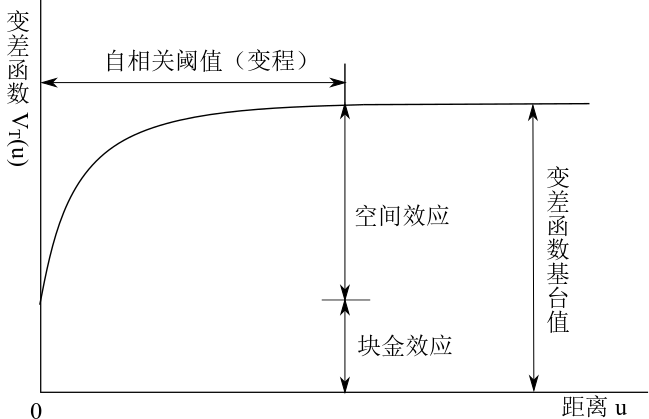
\includegraphics[width=0.7\linewidth]{figures/semi-variance} 

}

\caption{变差函数 $V_{T}(u)$ 示意图}\label{fig:semi-variance}
\end{figure}

常见的自协方差函数有三类,分别是高斯型协方差函数、球面型协方差函数和
Matérn 型协方差函数,由于 Matérn 型协方差函数的广泛应用性
\citep{Diggle1998, Diggle2002Childhood, Christensen2004},这里主要介绍它的有关性质特点。
\begin{equation}
\rho(u)=\{2^{\kappa -1}\Gamma(\kappa)\}^{-1}(u/\phi)^{\kappa}\mathcal{K}_{\kappa}(u/\phi),u > 0 \label{eq:matern1}
\end{equation} \noindent 一般地,假定 \(\rho(u)\)
单调不增,即任何两样本之间的相关性应该随距离变大而减弱,尺度参数
\(\phi\) 控制函数 \(\rho(u)\) 递减到0的速率。方便起见,记
\(\rho(u) = \rho_{0}(u/\phi)\),则方程 \eqref{eq:matern1} 可简记为
\begin{equation}
\rho_{0}(u)=\{2^{\kappa -1}\Gamma(\kappa)\}^{-1}(u)^{\kappa}\mathcal{K}_{\kappa}(u),u > 0 \label{eq:matern2}
\end{equation} \noindent 其中,\(\mathcal{K}_{\kappa}(\cdot)\) 是阶数为
\(\kappa\) 的第二类修正的贝塞尔函数(详见第 \ref{prepare}
章第\ref{sec:modified-bessel-function} 节), \(\kappa(>0)\)
是平滑参数,满足这些条件的空间过程 \(\mathcal{S}\) 是
\(\lceil\kappa\rceil-1\) 次均方可微的。值得注意的是 Matérn
族其实包含幂指数族 \noindent 当
\(\kappa = 0.5\)时,\(\rho_{0}(u) = \exp(-u)\), \(S(x)\)
均方连续但是不可微,当 \(\kappa \to \infty\) 时,
\(\rho_{0}(u) = \exp(-u^2)\), \(S(x)\)
无限次均方可微\citep{Diggle2007}。

在实际数据分析中,估计 \(\kappa\)
时,为了节省计算,又不失一般性,经验做法是取离散的 \(\kappa\) 值,如
\(\kappa = 0.5, 1.5, 2.5\),
这样,平稳空间高斯过程就分别具有均方连续不可微、一次可微和二次可微三种不同程度的光滑性。根据第
\ref{prepare} 章第 \ref{sec:stationary-gaussian-process} 节定理
\ref{thm:stationary-mean-square-properties},自相关函数 \(\rho(u)\)
的可微性表示了空间过程 \(\mathcal{S}\) 的曲面平滑程度。为更加直观地观察
\(\rho(u)\),作图 \ref{fig:matern-2d} 和图 \ref{fig:matern-3d}。

\begin{figure}

{\centering 
\includegraphics[width=0.8\linewidth]{figures/matern} 

}

\caption{左图:固定尺度参数 $\phi$,自相关函数 $\rho(u)$ 随空间距离 $u$ 的变化;右图:固定贝塞尔函数的阶 $\kappa$,自相关函数$\rho(u)$ 随空间距离 $u$ 的变化}\label{fig:matern-2d}
\end{figure}
\begin{figure}

{\centering 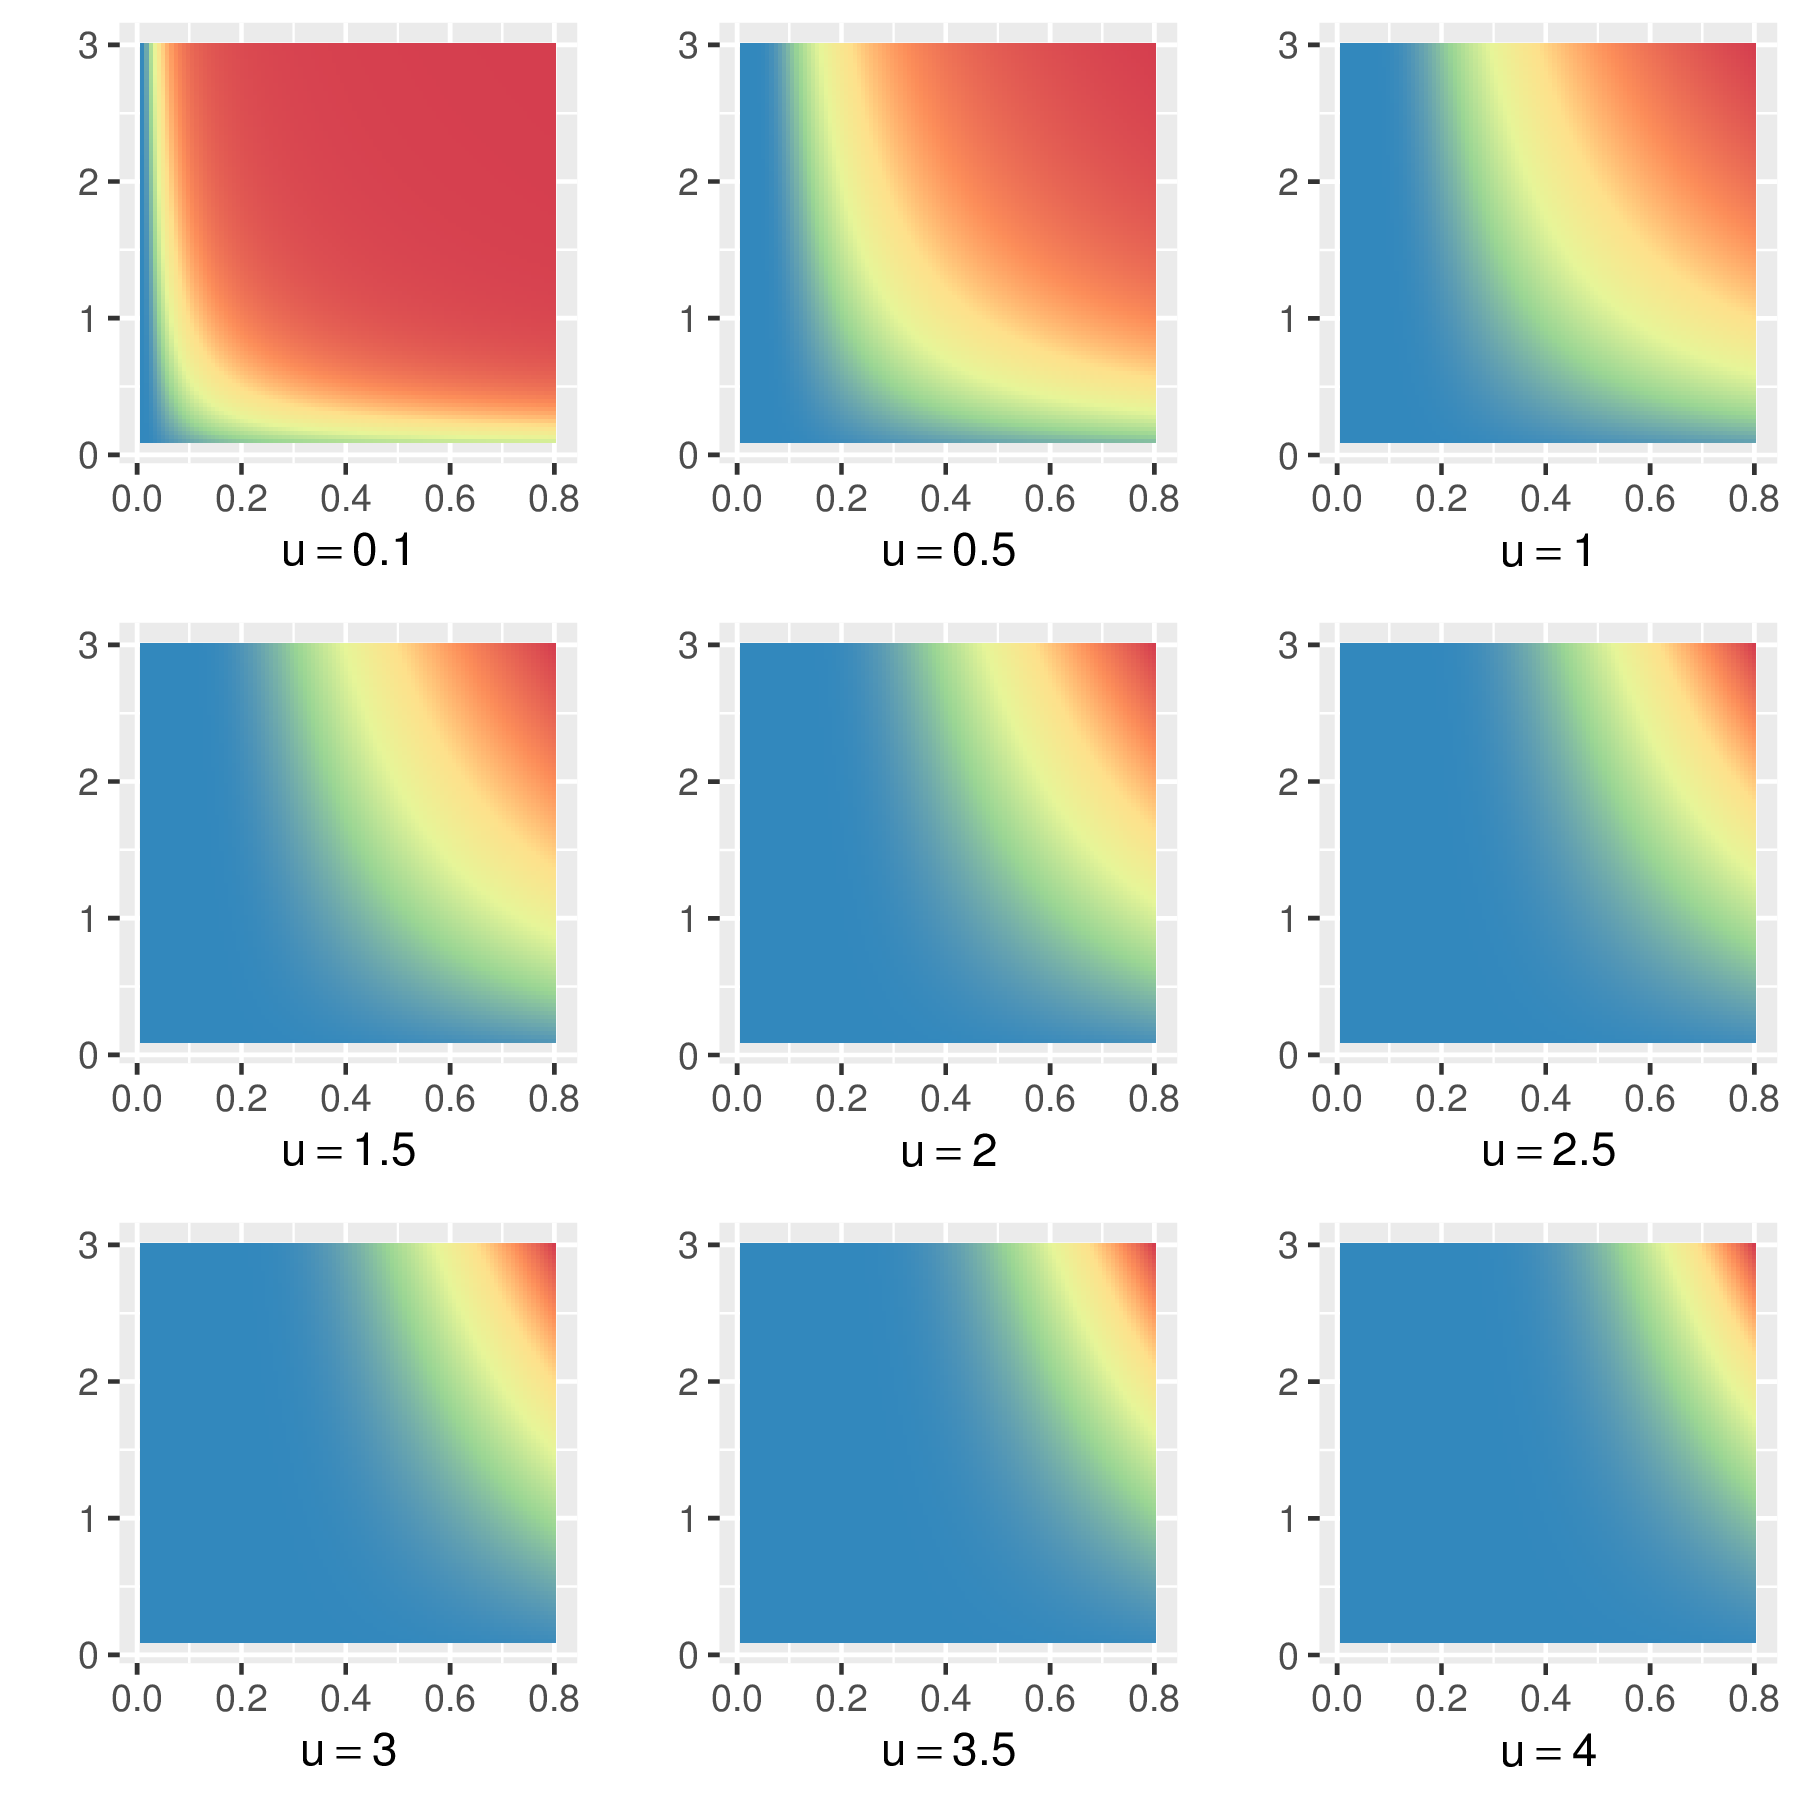
\includegraphics[width=0.8\linewidth]{figures/matern-3d} 

}

\caption{自相关函数 $\rho(u)$ 在不同空间距离$\mathsf{u}$处随贝塞尔函数的阶 $\kappa$ 和尺度参数 $\phi$ 的变化,横轴表示尺度参数 $\phi$,纵轴表示贝塞尔函数的阶$\kappa$,我们用 从蓝到红的颜色变化表示自相关函数 $\rho(u)$ 值由小到大,即表示相关性由弱变强}\label{fig:matern-3d}
\end{figure}

从图\ref{fig:matern-2d}可以看出,相比于贝塞尔函数的阶 \(\kappa\),
尺度参数 \(\phi\)
对相关函数的影响大些,由图\ref{fig:matern-2d}看出随着空间距离的增加,相关性减弱地特别快。在实际应用中,先固定下
\(\kappa\) 是可以接受的,为简化编程和表述,Diggle 等 (1998年)
\citep{Diggle1998} 在真实数据分析中使用幂指数型自相关函数
\(\rho_{0}(u) = \exp(-(\alpha u)^{\delta}), \alpha > 0, 0 < \delta \leq 2\)。
虽然其形式大大简化, 但函数图像和性质却与梅隆型有相似之处, 即当
\(0 < \delta < 2\) 时, \(S(x)\) 均方连续但不可微,当 \(\delta = 2\)
时, \(S(x)\) 无限次可微。

\hypertarget{subsec:identify}{%
\subsection{模型识别}\label{subsec:identify}}

在 SGLMM 模型的实际应用当中,一般先不添加非空间的随机效应,而是基于模型
\eqref{eq:no-nugget-SGLMM} 估计参数,估计完参数,代入模型,观察线性预测
\(\hat{T_{i}}\) 和真实的 \(T_i\)
之间的残差,如残差表现不平稳,说明还有非空间的随机效应没有提取,因此添加块金效应是合理的,此时在模型
\eqref{eq:SGLMM} 中有两个来源不同的随机效应 \(Z_{i}\) 与 \(S(x_i)\)。
\begin{equation}
g(\mu_i) = d(x_i)^{\top}\boldsymbol{\beta} + S(x_i) \label{eq:no-nugget-SGLMM}
\end{equation} 如何区分开 \(Z_{i}\) 与
\(S(x_i)\),或者更直接地说,如何估计这两个随机效应的参数
\(\tau^2, \sigma^2, \phi\), 即为可识别问题。 向量
\(T = (T_1,T_2,\ldots,T_n)^{\top}\) 是协方差为矩阵
\(\tau^2I + \sigma^2R\) 的多元高斯分布, 其中, 自相关函数
\(R_{ij} = \rho(u_{ij}; \phi)\), \(u_{ij}\) 是 \(x_i\) 与 \(x_j\)
之间的距离,由线性预测 \(T_{i}\) 的变差公式 \eqref{eq:variograms}
知,随机过程 \(T(x)\) 的变差 \(\tau^2 + \sigma^2(1-\rho(u_{ij}))\)
和自相关函数 \eqref{eq:corr-nugget-function} \begin{equation}
\rho^{\star}(u) =
\begin{cases}
                                     1 & : x_{i} = x_{j}  \\
\sigma^2\rho(u_{ij})/(\sigma^2+\tau^2) & : x_{i} \neq x_{j}
\end{cases} \label{eq:corr-nugget-function}
\end{equation} \noindent 在原点不连续,只有当
\(\tau^2 = \mathsf{Var}[Y_i|S(x_i)]\)
已知或者在同一位置可以用重复测量的方法直接获得时,参数
\(\tau^2, \sigma^2, \phi\) 是可识别的
\citep{Diggle2002Childhood, Diggle2007}。如果通过探索性数据分析观察到不可忽略的非空间效应
\(\tau^2\) 时,Christensen (2004年) \citep{Christensen2004}
建议使用样本变差函数对 \(\tau^2\) 作初步估计,然后计算关于 \(\tau^2\)
的剖面似然函数曲线,或者协方差参数 \(\phi,\tau^2\)一起确定最佳的值,第
\ref{applications} 章第 \ref{case-rongelap}
节将用剖面似然函数曲面的方法获取真实数据场景中的参数估计值。

\hypertarget{subsec:prior-sglmm}{%
\subsection{先验分布}\label{subsec:prior-sglmm}}

基于贝叶斯方法实现模型 \eqref{eq:SGLMM} 的参数估计,必然使用 MCMC
算法,自然地,需要指定模型参数
\(\boldsymbol{\theta} = (\boldsymbol{\beta},\tau^2,\sigma^2,\phi)\)
的先验分布。对于 \(\boldsymbol{\beta}\),Diggle 等 (2002 年)
\citep{Diggle2002Childhood} 选择相互独立的均匀先验,而对于参数
\(\tau^2,\sigma^2,\phi\),选取如下模糊先验:
\[f(\tau^2) \propto \frac{1}{\tau^2};f(\sigma^2) \propto \frac{1}{\sigma^2};f(\phi) \propto \frac{1}{\phi^2}\]
\noindent 其中,\(\tau^2\) 和 \(\sigma^2\) 为 Jeffreys 先验,Diggle 等
(2002 年) \citep{Diggle2002Childhood} 使用如下先验分布
\begin{equation*}
\log(\nu^2),\log(\sigma^2),\log(\phi)  \sim \mathcal{N}(\cdot,\cdot)
\end{equation*}
这些无信息先验分布的选择主要是出于实用和经验的考虑,也可以取别的,只要保持马尔科夫链收敛即可,实际操作中,我们还选取不同初始值,产生多条链,同时去掉迭代初始阶段产生的相对发散的参数迭代值,后续迭代值在链条收敛的情况下,可以把它当作后验分布产生的样本,然后依据该样本估计后验分布的参数。这些无信息先验分布的选择对最终结果几乎没有影响,这是贝叶斯方法的优势,也是贝叶斯推断方法得以被广泛应用的原因之一
\citep{mao2006}。

\hypertarget{sec:models}{%
\section{本章小结}\label{sec:models}}

本章第\ref{sec:Linear-Models}节至第\ref{sec:Generalized-Linear-Mixed-Effects-Models}节依次介绍了简单线性模型、广义线性模型和广义线性混合模型的结构,为引出本章第\ref{sec:Spatial-Generalized-linear-mixed-effects-models}节做准备,而且从统计建模和应用的角度,数据分析总是先从简单模型开始探索分析,一步步提取数据中的有用信息,本章正是循着这一思路介绍各个模型,这个想法也体现在第\ref{applications}章的真实数据分析过程中。

\hypertarget{algorithms}{%
\chapter{参数估计}\label{algorithms}}

模型的参数估计是建模分析的重要步骤,鉴于空间广义线性混合效应模型(简称
SGLMM)的复杂性,文献中的参数估计方法,如最小二乘估计(简称
LSE)和极大似然估计(简称 MLE)
都没有显式的表达式,因此必须发展有效的算法。目前,文献中的出现的算法有拉普拉斯近似算法、蒙特卡罗极大似然算法、贝叶斯马尔科夫链蒙特卡罗算法和低秩近似算法,应用这些算法去估计
SGLMM 模型参数,此外,特别提出了基于 Stan 实现的贝叶斯 MCMC
算法。第\ref{sec:mle}节和第\ref{sec:profile-likelihood}节分别介绍 SGLMM
模型的极大似然估计和空间线性混合模型下的剖面似然估计,由于估计中空间随机效应带来的高维积分问题,文献中出现了三类估计模型参数的算法,分别是第
\ref{subsec:LA} 小节介绍的拉普拉斯近似算法、第 \ref{subsec:MCML}
小节介绍的蒙特卡罗极大似然算法(简称 MCML), 第 \ref{sec:MCMC}
小节介绍的贝叶斯框架下的马尔科夫链蒙特卡罗算法 (简称贝叶斯 MCMC),第
\ref{LowRank} 小节介绍的低秩近似算法(简称 Low-Rank),在第
\ref{sec:STAN-MCMC} 节详细介绍在贝叶斯 MCMC 算法的基础上提出的 STAN-MCMC
算法。

\hypertarget{sec:mle}{%
\section{极大似然估计}\label{sec:mle}}

设研究区域 \(D \subseteq \mathbb{R}^2\), 对于第 \(i\) 次观测, \(s_i\)
表示区域 \(D\) 内的位置,\(Y(s_i)\)
表示响应变量,\(\mathbf{x}(s_i), i = 1, \ldots, n\) 是一个 \(p\)
维的固定效应,定义如下的 SGLMM 模型:

\[ \mathrm{E}[Y(s_i)|u(s_i)] = g^{-1}[\mathbf{x}(s_i)'\boldsymbol{\beta} + \mathbf{u}(s_i)], \quad i = 1, \ldots, n \]

\noindent 其中 \(g(\cdot)\) 是实值可微的逆联系函数, \(\beta\) 是 \(p\)
维的回归参数,代表 SGLMM
模型的固定效应。\(\{U(\mathbf{s}): \mathbf{s} \in D\}\)
是平稳的空间高斯过程,其均值为 \(\mathbf{0}\), 自协方差函数
\(\mathsf{Cov}(U(\mathbf{s}),U(\mathbf{s}')) = C(\mathbf{s} - \mathbf{s}'; \boldsymbol{\theta})\),
\(\boldsymbol{\theta}\) 是其中的参数向量。
\(\mathbf{u} = (u(s_1),u(s_2),\ldots,u(s_n))'\) 是平稳空间高斯过程
\(U(\cdot)\) 的一个实例。\(Y(\cdot)|U(\cdot)\) 是独立随机过程,如给定
\(\mathbf{u}\),观察值 \(\mathbf{y} = (y(s_1),y(s_2),\ldots,y(s_n))'\)
是相互独立的。

给定 \(u_i = u(s_i), i = 1, \ldots, n\), \(y_i = y(s_i)\)
的条件概率密度函数是
\[f(y_i|u_i;\boldsymbol{\beta}) = \exp[a(\mu_i)y_i - b(\mu_i)]c(y_i)\]
这里 \(\mu_i = Y_i|u_i\), \(a(\cdot),b(\cdot)\) 和 \(c(\cdot)\)
是特定的函数,具体的情况视所服从的分布而定,第\ref{prepare}章第\ref{sec:exp}节就不同的分布给出了不同函数形式。
SGLMM 模型的边际似然函数 \begin{equation}
L(\boldsymbol{\psi};\mathbf{y}) = \int \prod_{i=1}^{n} f(y_i|u_i;\boldsymbol{\beta})\phi_{n}(\mathbf{u};0,\Sigma_{\boldsymbol{\theta}})\mathrm{d}\mathbf{u} \label{eq:likelihood-function-1}
\end{equation} \noindent 其中
\(\boldsymbol{\psi} = (\boldsymbol{\beta},\boldsymbol{\theta})\) 是
SGLMM 模型的参数, \(\phi_{n}(\cdot;0,\Sigma_{\boldsymbol{\theta}})\)
表示 \(n\) 元正态密度函数,其均值为 \(\mathbf{0}\), 协方差矩阵为
\(\Sigma_{\boldsymbol{\theta}} = (c_{ij}) = (C(s_i - s_j; \boldsymbol{\theta})), i,j = 1, \ldots, n\)。
边际似然函数 \eqref{eq:likelihood-function-1}
几乎总是卷入一个难以处理的积分,这是主要面临的问题,并且计算量随观测
\(y_i\) 的数量增加,因为此积分的维数等于观测点的个数\citep{Diggle2007}。

再从贝叶斯方法的角度来看 SGLMM 模型, 令
\(\mathbf{y} = (y(s_1),\ldots,y(s_n))'\) 表示观测值,
\(\pi(\boldsymbol{\psi})\)
表示模型参数的联合先验密度,那么联合后验密度为 \begin{equation}
\begin{aligned}
\pi(\boldsymbol{\psi},\mathbf{u}|\mathbf{y}) &= \frac{f(\mathbf{y|\mathbf{u}, \boldsymbol{\psi}})\phi_{n}(\mathbf{u};0,\Sigma_{\boldsymbol{\theta}})\pi(\boldsymbol{\psi})}{m(\mathbf{y})} \\
m(\mathbf{y}) &= \int f(\mathbf{y|\mathbf{u}, \boldsymbol{\psi}})\phi_{n}(\mathbf{u};0,\Sigma_{\boldsymbol{\theta}})\pi(\boldsymbol{\psi})\mathrm{d} \mathbf{u} \mathrm{d} \boldsymbol{\psi}
\end{aligned}
\end{equation} \noindent 同样遭遇难以处理的高维积分问题,所以
\(m(\mathbf{y})\) 亦不会有显式表达式。特别地,若取
\(\pi(\boldsymbol{\psi})\) 为扁平先验 (flat priors) ,如
\(\pi(\boldsymbol{\psi}) \propto 1\), 后验分布将简化为似然函数
\eqref{eq:likelihood-function-1} 的常数倍。 如果导出的后验是合适的, MCMC
算法可以用来研究似然函数, 但是对很多 SGLMM
模型扁平先验会导出不合适的后验 (improper posteriors)
\citep{Natarajan1995}, 所以选用模糊先验 (diffuse
prior)来导出合适的后验 (proper
posteriors),导出的后验能接近似然函数,并不要求后验模 (posterior
mode) 完全是似然函数的极大似然估计 MLE \citep{Robert1996JASA}。

\hypertarget{sec:profile-likelihood}{%
\section{剖面似然估计}\label{sec:profile-likelihood}}

极大似然估计是一种被广泛接受的参数估计方法,因其优良的大样本性质,在宽松的正则条件下,极大似然估计服从渐近正态分布,满足无偏性,而且是有效的估计。为了叙述方便,似然函数能有显式表达式,考虑空间线性混合效应模型,即响应变量服从正态分布的情况,以此来介绍剖面似然估计
(profile likelihood estimate)\citep{Diggle2007}。 \begin{equation}
\mathbf{Y} \sim \mathcal{N}(D\boldsymbol{\beta},\sigma^2 \mathbf{R}(\phi) + \tau^2\mathbf{I})
\label{eq:gaussian-model}
\end{equation} \noindent 其中, \(D\) 是 \(n \times p\)
的观测数据矩阵,\(\boldsymbol{\beta}\)
是相应的回归参数向量,\(\mathbf{R}\) 依赖于 \(\phi\),\(\phi\)
可能含有多个参数。模型 \eqref{eq:gaussian-model} 的对数似然函数
\begin{equation}
\begin{aligned}
L(\boldsymbol{\beta},\tau^2,\sigma^2,\phi) = {} 
 & - 0.5\{ n\log(2\pi) + \log\{|(\sigma^2\mathbf{R}(\phi)+\tau^2\mathbf{I})|\} \\
 & + (\mathbf{Y} - D\boldsymbol{\beta})^{\top}(\sigma^2\mathbf{R}(\phi)+\tau^2\mathbf{I})^{-1}(\mathbf{Y} - D\boldsymbol{\beta}) \}  
\end{aligned} \label{eq:gauss-log-lik}
\end{equation} \noindent 极大化 \eqref{eq:gauss-log-lik} 式就是求模型
\eqref{eq:gaussian-model}
参数的极大似然估计,极大化对数似然的过程分步如下:

\begin{enumerate}
\def\labelenumi{\arabic{enumi}.}
\tightlist
\item
  重参数化 \(\nu^2 = \tau^2/\sigma^2\),令
  \(V = \mathbf{R}(\phi) + \nu^2 \mathbf{I}\);
\item
  给定 \(V\),对数似然函数 \eqref{eq:gauss-log-lik} 在 \begin{equation}
  \begin{aligned}
     \hat{\boldsymbol{\beta}}(V) & =  (D^{\top} V^{-1} D)^{-1} D^{\top} V^{-1}\mathbf{Y} \\
     \hat{\sigma}^2(V)           & =  n^{-1} \{\mathbf{Y} - D\hat{\boldsymbol{\beta}}(V)\}^{\top} V^{-1} \{\mathbf{Y} - D\hat{\boldsymbol{\beta}}(V)\}
  \end{aligned} \label{eq:beta-sigma}
  \end{equation} 取得极大值;
\item
  将 \eqref{eq:beta-sigma} 式代入对数似然函数 \eqref{eq:gauss-log-lik}
  式,可获得一个简化的对数似然 \begin{equation}
     L_{0}(\nu^2,\phi) = - 0.5\{ n\log(2\pi) + n\log \hat{\sigma}^2(V) + \log |V| + n \} \label{eq:reduced-gauss-log-lik}
  \end{equation}
\item
  关于参数 \(\nu^2, \phi\) 极大化 \eqref{eq:reduced-gauss-log-lik}
  式,获得参数 \(\nu^2, \phi\) 的估计值,再将其回代 \eqref{eq:beta-sigma}
  式,获得估计值 \(\hat{\boldsymbol{\beta}}\) 和 \(\hat{\sigma}^2\)。
\end{enumerate}

在空间线性混合效应模型的设置下,上述极大化似然函数的过程可能与自协方差函数的类型有关,如在使用
Matérn 型自协方差函数的时,形状参数(shape parameter) \(\kappa\)
也卷入到 \(\phi\) 中,导致识别问题。因此,让 \(\kappa\) 分别取
\(0.5,1.5,2.5\),使得平稳空间高斯过程 \(\mathcal{S}\)
覆盖到不同程度的均方可微性
\citep{Warnes1987}。原则上,极大似然估计的变化情况可以通过观察对数似然函数的曲面来分析\footnote{SGLMM
  模型的似然函数通常不止一个极值点},但是,似然曲面的维数往往不允许直接观察。在这种情形下,另一个基于似然的想法是剖面似然
(profile likelihood)。一般地,假定我们有一个模型,其含有参数
\((\alpha,\phi)\),似然表示为 \(L(\alpha,\phi)\)。则关于 \(\alpha\)
的剖面似然函数定义为 \begin{equation}
L_{p}(\alpha) = L(\alpha,\hat{\psi}(\alpha)) = \max_{\psi} (L(\alpha,\psi))
\label{eq:profile-log-lik}
\end{equation} \noindent 即考虑似然函数随 \(\alpha\)
的变化情况,对每一个 \(\alpha\) (保持 \(\alpha\) 不变),指定 \(\psi\)
的值使得对数似然取得最大值。剖面似然就是让我们可以观察到关于 \(\alpha\)
的似然曲面,显然,其维数比完全似然面要低,与只有一个参数的对数似然一样,它也可以用来计算单个参数的置信区间。现在,注意到简化的对数似然
\eqref{eq:reduced-gauss-log-lik} 其实可以看作模型 \eqref{eq:gaussian-model}
关于 \((\nu^2,\phi)\) 的剖面对数似然 \citep{Diggle2007}。

\hypertarget{sec:algrithms}{%
\section{参数估计的算法}\label{sec:algrithms}}

\hypertarget{subsec:LA}{%
\subsection{拉普拉斯近似算法}\label{subsec:LA}}

为描述拉普拉斯近似算法,空间广义线性混合效应模型(简称
SGLMM)的结构重新表述如下: \begin{equation}
\begin{aligned}
\mathbf{Y(x)} | S(\mathbf{x}) & \sim  f(\cdot;\boldsymbol{\mu(x)},\psi) \\
g(\boldsymbol{\mu(x)}) & =  D\boldsymbol{\beta} + S(\mathbf{x}) 
                         = D\boldsymbol{\beta} + \sigma R(\mathbf{x};\phi) + \tau z \\
S(\mathbf{x}) & \sim  \mathcal{N}(\mathbf{0},\Sigma)
\end{aligned} \label{eq:sglmm}
\end{equation}

\noindent SGLMM 模型假定在给定高斯空间过程 \(S(\mathbf{x})\) 的条件下,
\(Y_1,Y_2,\ldots,Y_n\) 是独立的,并且服从分布
\(f(\cdot;\boldsymbol{\mu(x)},\psi)\)。此分布的参数有两个来源,其一是与联系函数
\(g\) 关联的线性预测 \(\boldsymbol{\mu(x)}\),其二是密度分布函数 \(f\)
的发散参数 \(\psi\),可以看作是似然函数中的附加参数。空间过程
\(S(\mathbf{x})\) 分解为空间相关 \(R(\mathbf{x};\phi)\) 和独立过程
\(Z\),二者分别被参数 \(\sigma\) 和 \(\tau\)
归一化而具有单位方差。线性预测包含一组固定效应
\(D\boldsymbol{\beta}\),空间相关的随机效应
\(R(\mathbf{x};\phi)\),与空间不相关的随机效应
\(\tau z \sim \mathcal{N}(\mathbf{0},\tau^2\mathbf{I})\)。\(D\)
是根据协变量观测值得到的数据矩阵,\(\boldsymbol{\beta}\) 是
\(p \times 1\) 维的回归参数向量。

\(R(\mathbf{x};\phi)\) 是具有单位方差的平稳空间高斯过程,其自相关函数为
\(\rho(u,\phi)\),这里 \(u\) 表示一对空间位置之间的距离,\(\phi\)
是刻画空间相关性的参数。自相关函数 \(\rho(u,\phi) (\in \mathbb{R}^d)\)
是 \(d\) 维空间到一维空间的映射函数,特别地,假定空间过程
\(S(\mathbf{x})\)的自相关函数仅仅依赖成对点之间的欧氏距离,即
\(u =\|x_i - x_j\|\)。常见的自相关函数有指数型、梅隆型和球型。线性预测的随机效应部分协方差矩阵
\(\Sigma = \sigma^2 R(\mathbf{x};\phi) + \tau^2\mathbf{I}\)。

估计 SGLMM 模型 \eqref{eq:sglmm} 的参数
\(\boldsymbol{\theta} = (\boldsymbol{\beta},\sigma^2,\tau^2,\phi,\psi)\)
需要极大化边际似然函数 \begin{equation}
L(\boldsymbol{\theta};\mathbf{y}) = \int_{\mathbb{R}^n} [\mathbf{Y(x)}|S(\mathbf{x})][S(\mathbf{x})]\mathrm{d}S(\mathbf{x}) \label{eq:marginal-likelihood}
\end{equation} \noindent 其中,符号 \([\cdot]\)
表示随机变(向)量的分布,一般地,边际似然函数\(L(\boldsymbol{\theta};\mathbf{y})\)包含两个分布的乘积和随机效应的积分,并且这个积分无法显式的表示,第一个分布是观测变量
\(\mathbf{Y}\) 的抽样分布,第二个分布是多元高斯分布。一个特殊的情况是
\(\mathbf{Y}\) 也假设服从多元高斯分布,这时积分有显式表达式。

边际似然函数 \eqref{eq:marginal-likelihood}
卷入的数值积分是充满挑战的,因为积分的维数 \(n\)
是观测值的数目,所以像二次、高斯-埃尔米特或适应性高斯-埃尔米特数值积分方式都是不可用的,Tierney
和 Kadane (1986 年)提出拉普拉斯近似方法
\citep{Tierney1986},它在纵向数据分析中被大量采用
\citep{Diggle2002Analysis}。总之,对空间广义线性混合效应模型而言,拉普拉斯近似还可以继续采用,想法是近似边际似然函数中的高维
\((n > 3)\)
积分,获得一个易于处理的表达式,有了积分的显式表达式,就可以用数值的方法求边际似然函数的极大值。拉普拉斯方法即用如下方式近似
\eqref{eq:marginal-likelihood} 中的积分 \begin{equation}
I   =  \int_{\mathbb{R}^n} \exp\{Q(\mathbf{s})\}\mathrm{d}\mathbf{s} 
  \approx  (2\pi)^{n/2} |-Q''(\hat{\mathbf{s}})|^{-1/2}\exp\{Q(\hat{\mathbf{s}})\} \label{eq:laplace-approximate}
\end{equation} \noindent 其中,\(Q(\mathbf{s})\) 为已知的 \(n\)
元函数,\(\hat{\mathbf{s}}\) 是其极大值点,\(Q''(\hat{\mathbf{s}})\)
是黑塞矩阵。拉普拉斯近似的一维情形和主要近似的想法已在第\ref{prepare}章第\ref{sec:Laplace-approximation}节详细阐述。

拉普拉斯近似方法也可以用于一般的广义线性混合效应模型的似然推断,特别地,对于空间广义线性混合效应模型,假定条件分布
\(f\) 可以表示成如下指数族的形式 \begin{equation}
f(\mathbf{y};\boldsymbol{\beta})  = \exp\{\mathbf{y}^{\top} (D\boldsymbol{\beta} + S(\mathbf{x})) - \mathbf{1}^{\top} b( D\boldsymbol{\beta} + S(\mathbf{x})) + \mathbf{1}^{\top} c(\mathbf{y}) \}  \label{eq:exponential-family}
\end{equation} \noindent 其中 \(b(\cdot)\)
是特定的函数,常用的分布有泊松分布和二项分布等,详见第\ref{prepare}章第\ref{sec:exp}节。把
\eqref{eq:marginal-likelihood} 式中关于 \([S(\mathbf{x})]\)
多元高斯密度函数表示为 \begin{align}
f(S(\mathbf{x});\Sigma) & = (2\pi)^{-n/2}|\Sigma|^{-1/2} \exp\{ -\frac{1}{2}S(\mathbf{x})^{\top} \Sigma^{-1} S(\mathbf{x}) \} \\
                      & = \exp\{ - \frac{n}{2}\log (2\pi) -\frac{1}{2}\log |\Sigma|  -\frac{1}{2}S(\mathbf{x})^{\top} \Sigma^{-1} S(\mathbf{x}) \} \label{eq:multi-gaussian-dist}
\end{align} \noindent 现在将边际似然函数 \eqref{eq:marginal-likelihood}
写成适合使用拉普拉斯近似的格式 \begin{equation}
L(\boldsymbol{\theta};\mathbf{y}) = \int_{\mathbb{R}^n} \exp\{Q(S(\mathbf{x}))\} \mathrm{d}S(\mathbf{x}) 
\end{equation} \noindent 其中 \begin{equation}
\begin{aligned}
Q(S(\mathbf{x})) ={} &  \mathbf{y}^{\top} (D \boldsymbol{\beta} + S(\mathbf{x})) - \mathbf{1}^{\top} b(D \boldsymbol{\beta} + S(\mathbf{x})) + \mathbf{1}^{\top}c(\mathbf{y}) \\
                   & - \frac{n}{2}\log (2\pi) -\frac{1}{2}\log |\Sigma| -\frac{1}{2}S(\mathbf{x})^{\top} \Sigma^{-1} S(\mathbf{x})
\end{aligned} \label{eq:log-lik}
\end{equation} \noindent 方程 \eqref{eq:log-lik}
凸显了采纳拉普拉斯近似方法拟合空间广义线性混合效应模型的方便性,可以把
\eqref{eq:log-lik}
当成两部分来看,前一部分是广义线性模型下样本的对数似然的和的形式,后一部分是多元高斯分布的对数似然。要使用
\eqref{eq:laplace-approximate} 式,需要函数 \(Q(S(\mathbf{x}))\)
的极大值点 \(\hat{\mathbf{s}}\),这里采用牛顿-拉夫森算法
(Newton-Raphson,简称 NR) 寻找 \(n\) 元函数的极大值点,NR
算法需要重复计算 \begin{equation}
\mathbf{s}_{i+1} = \mathbf{s}_{i} - Q''(\mathbf{s}_{i})^{-1}Q'(\mathbf{s}_{i}) 
\end{equation} \noindent 一直收敛到
\(\hat{\mathbf{s}}\)。在这个内迭代的过程中,将参数
\(\boldsymbol{\theta}\) 当作已知的。\(Q\) 函数的一阶和二阶导数如下
\begin{align}
Q'(\mathbf{s})& =  \{\mathbf{y} - b'(D\boldsymbol{\beta} + \mathbf{s}) \}^{\top} - \mathbf{s}^{\top}\Sigma^{-1} \label{eq:first-deriv} \\
Q''(\mathbf{s})& =  -\mathrm{diag} \{b''(D\boldsymbol{\beta} + \mathbf{s}) \} - \Sigma^{-1} \label{eq:second-deriv}
\end{align}
\noindent 用拉普拉斯方法近似的对数似然\(\ell(\boldsymbol{\theta};\mathbf{y})\)
\begin{equation}
\begin{aligned}
\ell(\boldsymbol{\theta};\mathbf{y}) = {} & \frac{n}{2}\log (2\pi) -\frac{1}{2}\log | -\mathrm{diag} \{b''(D\boldsymbol{\beta} + \mathbf{s}) \} - \Sigma^{-1} |  \\
& + \mathbf{y}^{\top} (D\boldsymbol{\beta} + \hat{\mathbf{s}}) - \mathbf{1}^{\top} b( D\boldsymbol{\beta} + \hat{\mathbf{s}}) + \mathbf{1}^{\top} c(\mathbf{y}) \\
& - \frac{n}{2}\log (2\pi) -\frac{1}{2}\log |\Sigma| -\frac{1}{2}\hat{\mathbf{s}}^{\top} \Sigma^{-1} \hat{\mathbf{s}}
\end{aligned} \label{eq:approx-log-lik}
\end{equation} \noindent 现在极大化近似对数似然 \eqref{eq:approx-log-lik}
式,此时是求模型参数,可称之为外迭代过程,常用的算法是
Broyden-Fletcher-Goldfarb-Shanno (简称BFGS) 算法,它内置在 R 函数
\texttt{optim()} 中。方便起见,模型参数记为
\(\boldsymbol{\theta} = (\boldsymbol{\beta},\log(\sigma^2),\log(\tau^2),\log(\phi),\log(\psi))\),且
\(\hat{\boldsymbol{\theta}}\) 表示 \(\boldsymbol{\theta}\)
的最大似然估计,根据第\ref{prepare}章第\ref{sec:def-mle}节定理\ref{thm:asymptotic-normality},则
\(\hat{\boldsymbol{\theta}}\) 的渐进分布为
\[ \hat{\boldsymbol{\theta}} \sim \mathcal{N}(\boldsymbol{\theta}, \mathbf{I}_{o}^{-1}(\hat{\boldsymbol{\theta}})) \]
\noindent 其中 \(\mathbf{I}_{o}(\hat{\boldsymbol{\theta}})\)
为观察到的样本信息阵,注意到在空间广义线性混合效应模型下,不能直接计算
Fisher 信息阵,因为对数似然函数没有显式表达式,只有数值迭代获得在
\(\hat{\boldsymbol{\theta}}\)
处的观测信息矩阵。通常,这类渐进近似对协方差参数
\(\sigma^2, \tau^2, \phi\)
的估计效果不好,在数据集不太大的情形下,可用第
\ref{sec:profile-likelihood}
节介绍的剖面似然方法计算协方差参数及其置信区间。剖面似然估计的算法实现过程详见
Bolker 等 (2017年) 开发的 bbmle 包
\citep{R-bbmle},下面给出计算的细节步骤:

\begin{enumerate}
\def\labelenumi{\arabic{enumi}.}
\tightlist
\item
  选择模型参数 \(\boldsymbol{\theta}\) 的初始值
  \(\boldsymbol{\theta}_{i}\);
\item
  计算协方差矩阵 \(\Sigma\) 及其逆 \(\Sigma^{-1}\);
\item
  通过如下步骤极大\(Q\)函数,获得估计值 \(\hat{\mathbf{s}}\);

  \begin{enumerate}
  \def\labelenumii{(\alph{enumii})}
  \tightlist
  \item
    为 \(\mathbf{s}\) 选择初始值;
  \item
    按 \eqref{eq:first-deriv} 式计算 \(Q'(\mathbf{s})\),按
    \eqref{eq:second-deriv} 式计算
    \(Q''(\mathbf{s})\),其中导数计算的代码实现可参考黄湘云(2016年)
    \citep{Huang2016COS};
  \item
    解线性方程组
    \(Q''(\mathbf{s})\mathbf{s}^{\star} = Q'(\mathbf{s})\);
  \item
    更新 \(\mathbf{s = s + s^{\star}}\);
  \item
    迭代直到收敛以获得 \(\hat{\mathbf{s}}\)。
  \end{enumerate}
\item
  用 \(\hat{\mathbf{s}}\) 替换 \(S(\mathbf{x})\),在 \eqref{eq:log-lik}
  式中计算 \(Q(\hat{\mathbf{s}})\);
\item
  用 \eqref{eq:laplace-approximate} 式计算积分的近似值,以获得边际似然
  \eqref{eq:approx-log-lik} 式的值;
\item
  用 BFGS 算法获得下一个值 \(\boldsymbol{\theta}_{i+1}\);
\item
  重复上述过程直到收敛,获得参数的估计值 \(\hat{\boldsymbol{\theta}}\)。
\end{enumerate}

NR算法收敛速度是很快的,但是必须提供一个很好的初值,好的初值对于快速收敛到似然函数
\(\ell(\boldsymbol{\theta};\mathbf{y})\)
的极大值点很重要。指定外迭代中的初值
\(\boldsymbol{\theta}_{0}\)的一个策略是首先拟合一个简单的广义线性模型,获得回归系数
\(\boldsymbol{\beta}\) 的初值,基于这些值计算线性预测值
\(\hat{\boldsymbol{\mu}}\);然后计算残差
\(\hat{\boldsymbol{r}} = (\hat{\boldsymbol{\mu}} - \mathbf{y})\),
\(\hat{\boldsymbol{r}}\) 的方差作为 \(\sigma^2\) 的初值,如果 SGLMM
带有块金效应,就用 \(\sigma^2\) 的初值的一定比例,如 10\% 作为
\(\tau^2\) 的初值;最后,\(\phi\)
的初值选择两个距离最大的观测点之间的距离的
10\%,比较保险的办法是选择不同的 \(\phi\)
作为初值,这个过程需要不断的试错以期获得算法的收敛\citep{Bonat2016Practical}。

\hypertarget{subsec:MCML}{%
\subsection{蒙特卡罗极大似然算法}\label{subsec:MCML}}

为描述蒙特卡罗极大似然算法,空间广义线性混合效应模型的结构表述如下
\begin{equation}
g(\mu_i) = T_{i} = d(x_i)^{\top}\boldsymbol{\beta} + S(x_i) + Z_i \label{eq:again-SGLMM}
\end{equation} \noindent 其中,令
\(d_{i} = d(x_i)^{\top}\),用\(d(x_i)^{\top}\) 表示
主要是强调协变量的空间内容, 这里表示采样点处观测数据向量, 即 \(p\)
个协变量在第 \(i\) 个位置 \(x_i\) 的观察值。
\(\mathcal{S} = \{S(x): x \in \mathbb{R}^2\}\) 是均值为
\(\mathbf{0}\),方差为
\(\sigma^2\),平稳且各向同性的空间高斯过程,自相关函数是
\(\rho(u;\phi)\),\(S(x_i)\)
表示空间效应,\(Z_i \stackrel{i.i.d}{\sim} \mathcal{N}(0,\tau^2)\)
的块金效应,\(g\) 是联系函数,\(x_i \in \mathbb{R}^2\)是采样点的位置。
综上,模型 \eqref{eq:again-SGLMM} 待估计的参数有 \(\boldsymbol{\beta}\) 和
\(\boldsymbol{\theta}' = (\sigma^2,\phi,\tau^2)\)。
特别地,当响应变量分别服从二项分布和泊松分布时, 模型
\eqref{eq:again-SGLMM} 分别变为模型 \eqref{eq:BL-SGLMM} 和模型
\eqref{eq:Poss-SGLMM}。 \begin{align}
\log\{\frac{p_i}{1-p_i}\} & = T_{i} = d(x_i)^{\top}\boldsymbol{\beta} + S(x_i) + Z_i  \label{eq:BL-SGLMM}\\
\log(\lambda_i)           & = T_{i} = d(x_i)^{\top}\boldsymbol{\beta} + S(x_i) + Z_i  \label{eq:Poss-SGLMM}
\end{align} \noindent 模型 \eqref{eq:BL-SGLMM} 中,响应变量 \(Y_i\)
服从二项分布 \(Y_i \sim \mathrm{Binomial}(m_i,p_i)\), 均值
\(\mathsf{E}(Y_i|S(x_i),Z_i)=m_{i}p_{i}\), \(m_i\) 表示在 \(x_i\)
的位置抽取的样本量,总的样本量就是 \(M = \sum_{i=1}^{N}m_i\),\(N\)
表示采样点的个数。模型 \eqref{eq:Poss-SGLMM} 中, 响应变量 \(Y_i\)
服从泊松分布 \(Y_i \sim \mathrm{Poisson}(\lambda_i)\)。 在获取响应变量
\(Y\) 的观测的过程中,与广义线性或广义线性混合效应模型 \eqref{eq:GLM} 和
\eqref{eq:GLMM} 不同的在于:在每个采样点 \(x_i\) 处,\(Y_i\)
都服从参数不同但同类的分布。

模型 \eqref{eq:BL-SGLMM} 中参数 \(\boldsymbol{\beta}\) 和
\(\boldsymbol{\theta}^{\top} = (\sigma^2,\phi,\tau^2)\)
的似然函数是通过对 \(T_i\) 内的随机效应积分获得的。 用大写 \(D\) 表示
\(n\times p\) 的数据矩阵, \(y = (y_1, y_2,\cdots, y_n)\) 表示各空间位置
\(x_i\) 处响应变量的观测值,对应模型 \eqref{eq:BL-SGLMM} 中的
\(Y_i \sim \mathrm{Binomial}(m_i,p_i)\),
\(\mathbf{T} = (T_1,T_2,\ldots,T_n)\) 的边际分布是
\(\mathcal{N}(D\boldsymbol{\beta}, \Sigma(\boldsymbol{\theta}))\),
其中,协方差矩阵 \(\Sigma(\boldsymbol{\theta})\) 的对角元是
\(\sigma^2+\tau^2\), 非对角元是 \(\sigma^2\rho(u_{ij})\), \(u_{ij}\)
是位置 \(x_i\) 与 \(x_j\) 之间的距离。在给定
\(\mathbf{T} = t = (t_1,t_2,\cdots,t_n)\) 下,
\(\mathbf{Y} = y =(y_1,\cdots,y_n)\)
的条件分布是独立二项概率分布函数的乘积
\(f(y|t)=\prod_{i=1}^{n}f(y_{i}|t_{i})\), 因此, \(\boldsymbol{\beta}\)
和 \(\boldsymbol{\theta}\) 的似然函数可以写成 \begin{equation}
L(\boldsymbol{\beta},\boldsymbol{\theta}) = f(y;\boldsymbol{\beta},\boldsymbol{\theta}) = \int_{\mathbb{R}^{n}}\mathcal{N}(t;D\boldsymbol{\beta},\Sigma(\boldsymbol{\theta}))f(y|t)dt \label{eq:likelihood}
\end{equation} \noindent 其中\(\mathcal{N}(\cdot;\mu,\Sigma)\)
表示均值为 \(\mu\),协方差矩阵为 \(\Sigma\)
的多元高斯分布的密度函数。Geyer (1994 年)\citep{Geyer1994On} 在给定
\(\mathbf{Y}=y\) 的情况下,使用 \(\mathbf{T}\) 的条件分布
\(f(\mathbf{T}|\mathbf{Y}=y)\) 模拟近似方程 \eqref{eq:likelihood}
中的高维积分,则似然函数 \(L(\boldsymbol{\beta},\boldsymbol{\theta})\)
可以重写为 \begin{equation}
\begin{aligned}
L(\boldsymbol{\beta},\boldsymbol{\theta})
& = \int_{\mathbb{R}^{n}} \frac{\mathcal{N}(t;D\boldsymbol{\beta},\Sigma(\boldsymbol{\theta}))f(y|t)}{\mathcal{N}(t;D\boldsymbol{\beta}_{0},\Sigma(\boldsymbol{\theta}_{0}))f(y|t)}f(y,t)dt \\
& \varpropto \int_{\mathbb{R}^{n}} \frac{\mathcal{N}(t;D\boldsymbol{\beta}, \Sigma(\boldsymbol{\theta}))}{\mathcal{N}(t;D\boldsymbol{\beta}_{0}, \Sigma(\boldsymbol{\theta}_{0}))}f(t|y)dt \\
&= E_{T|y}\left[\frac{\mathcal{N}(t; D\boldsymbol{\beta}, \Sigma(\boldsymbol{\theta}))}{\mathcal{N}(t; D\boldsymbol{\beta}_{0}, \Sigma(\boldsymbol{\theta}_{0}))}\right] 
\end{aligned} \label{eq:likelihood2}
\end{equation} \noindent 其中
\(\boldsymbol{\beta}_{0},\boldsymbol{\theta}_{0}\)
作为迭代初始值预先给定,则 \(Y\) 和 \(T\) 的联合分布可以表示成
\(f(y,t) = \mathcal{N}(t; D\boldsymbol{\beta}_{0}, \Sigma(\boldsymbol{\theta}_{0})) f(y|t)\)。
再通过蒙特卡罗方法,用求和代替积分近似期望, 做法是从条件分布
\(f(T|Y=y; \boldsymbol{\beta}_0, \boldsymbol{\theta}_0)\) 抽取 \(m\)
个样本 \(t_{(i)}\), 那么,可以用方程 \eqref{eq:likelihood-approx}
近似方程 \eqref{eq:likelihood2} \begin{equation}
L_{m}(\boldsymbol{\beta},\boldsymbol{\theta})=\frac{1}{m}\sum_{i=1}^{n}\frac{\mathcal{N}(t_{i};D\boldsymbol{\beta},\Sigma(\boldsymbol{\theta}))}{\mathcal{N}(t_{i};D\boldsymbol{\beta}_{0},\Sigma(\boldsymbol{\theta}_{0}))} \label{eq:likelihood-approx}
\end{equation}

\noindent 这样做的依据是不管样本序列 \(t_{(i)}\) 是否相关,
\(L_{m}(\boldsymbol{\beta},\boldsymbol{\theta})\) 都是
\(L_{m}(\boldsymbol{\beta},\boldsymbol{\theta})\) 的一致估计
(consistent estimator)\citep{PrevMap2017JSS}。 最优的
\(\boldsymbol{\beta}_0,\boldsymbol{\theta}_0\) 是
\(\boldsymbol{\beta},\boldsymbol{\theta}\)
的极大似然估计,即\(\max_{\boldsymbol{\beta},\boldsymbol{\theta}}L_{m}(\boldsymbol{\beta},\boldsymbol{\theta}) \rightarrow 1, m \rightarrow\infty\)。

既然给定的初始值 \(\boldsymbol{\beta}_{0},\boldsymbol{\theta}_{0}\)
必定与真实的极大似然估计值不同,第 \(m\) 步迭代获得的似然函数值
\(L_{m}(\hat{\boldsymbol{\beta}}_{m}, \hat{\boldsymbol{\theta})}_{m}\)
与 1 的距离可以用来刻画蒙特卡罗近似的准确度。实际操作中,用
\(\hat{\boldsymbol{\beta}}_{m}\) 和 \(\hat{\boldsymbol{\theta}}_{m}\)
表示最大化 \(L_{m}(\boldsymbol{\beta}, \boldsymbol{\theta})\) 获得的
MCML 估计,重复迭代
\(\boldsymbol{\beta}_{0} = \hat{\boldsymbol{\beta}}_{m}\) 和
\(\boldsymbol{\theta}_{0} = \hat{\boldsymbol{\theta}}_{m}\) 直到收敛。
求蒙特卡罗近似的对数似然
\(l_{m}(\boldsymbol{\beta}, \boldsymbol{\theta}) = \log L_{m}(\boldsymbol{\beta}, \boldsymbol{\theta})\)
的极值,可以使用 PrevMap 包,迭代
\(L_{m}(\boldsymbol{\beta}, \boldsymbol{\theta})\) 的过程中,可以选择
BFGS 算法。关于 \(\boldsymbol{\psi}\)
的似然曲面是相当扁平的,为了更好的收敛到全局极大值,做一步重参数化,即令
\(\boldsymbol{\psi} = \log(\boldsymbol{\theta})\),\(L_{m}(\boldsymbol{\beta}, \boldsymbol{\psi})\)
关于 \(\boldsymbol{\beta}\) 和 \(\boldsymbol{\psi}\)
的一阶、二阶导数传递给 maxLik 包的 \texttt{maxBFGS} 函数。

蒙特卡罗极大似然估计 \(\boldsymbol{\theta}_{m}\) 的标准误差 (standard
errors) 取似然函数 \(l_{m}(\boldsymbol{\beta},\boldsymbol{\theta})\)
的负黑塞矩阵的逆的对角线元素的平方根。迭代次数足够多时,即 \(m\)
充分大时,一般取到 10000 及以上,此时蒙特卡罗误差可忽略,即用方程
\eqref{eq:likelihood-approx} 近似 \eqref{eq:likelihood2} 的误差可忽略。

\hypertarget{sec:MCMC}{%
\subsection{贝叶斯 MCMC 算法}\label{sec:MCMC}}

在贝叶斯框架里,\(\boldsymbol{\beta}, \boldsymbol{\theta}\)
的后验分布由贝叶斯定理和 \(\boldsymbol{\beta}, \boldsymbol{\theta}\)
的联合先验分布确定,见第\ref{prepare}章基础知识第\ref{sec:bayes-prior}节后验分布的推导。假定
\(\boldsymbol{\beta}, \boldsymbol{\theta}\) 的先验分布如下:
\[ \boldsymbol{\theta} \sim  g(\cdot), \quad \boldsymbol{\beta} | \sigma^2 \sim  \mathcal{N}(\cdot; \xi, \sigma^2 \Omega) \]
\noindent 其中 \(g(\cdot)\) 可以是 \(\boldsymbol{\theta}\)
的任意分布,\(\xi\) 和 \(\Omega\) 分别是 \(\boldsymbol{\beta}\)
的高斯先验的均值向量和协方差矩阵。则\(\boldsymbol{\beta}, \boldsymbol{\theta}\)
和 \(\mathbf{T}\) 的后验分布是 \begin{equation}
\pi(\boldsymbol{\beta}, \boldsymbol{\theta}, t | y) \propto g(\boldsymbol{\theta})\mathcal{N}(\boldsymbol{\beta}; \xi, \sigma^2 \Omega)\mathcal{N}(t; D\boldsymbol{\beta}, \Sigma(\boldsymbol{\theta}))f(y|t) \label{eq:posterior}
\end{equation} \noindent R 包 PrevMap 内的函数
\texttt{binomial.logistic.Bayes}
可以从上述后验分布中抽得样本,这个抽样的过程使用了 MCMC 算法,
\(\boldsymbol{\theta}, \boldsymbol{\beta}\) 和 \(\mathbf{T}\)
轮流迭代的过程如下:

\begin{enumerate}
\def\labelenumi{\arabic{enumi}.}
\tightlist
\item
  初始化\(\boldsymbol{\beta}, \boldsymbol{\theta}\) 和\(\mathbf{T}\);
\item
  对协方差\(\Sigma(\boldsymbol{\theta})\)中的参数做如下变换
  \citep{Christensen2006}
  \[(\tilde{\theta}_{1}, \tilde{\theta}_{2}, \tilde{\theta}_{3}) = (\log \sigma, \log (\sigma^2/\phi^{2\kappa}), \log \tau^2)\]
  使用随机游走 Metropolis-Hastings 算法轮流更新上述三个参数,在第 \(i\)
  次迭代时,候选高斯分布的标准差 \(h\) 是
  \(h_{i} = h_{i-1} + c_{1}i^{-c_{2}}(\alpha_{i}-0.45)\),其中,\(c_{1} > 0\)
  和 \(c_{2} \in (0,1]\) 是预先给定的常数,\(\alpha_i\) 是第 \(i\)
  次迭代时的接受概率,其中 0.45 是一元高斯分布的最优接受概率;
\item
  使用Gibbs步骤更新 \(\boldsymbol{\beta}\), 所需条件分布
  \(\boldsymbol{\beta}|\boldsymbol{\theta},\mathbf{T}\) 是高斯分布,均值
  \(\tilde{\xi}\),协方差矩阵 \(\sigma^2\tilde{\Omega}\),且与 \(y\)
  不相关,记\(\Sigma(\boldsymbol{\theta}) = \sigma^2 R(\boldsymbol{\theta})\)
  \[ \tilde{\xi}  =  \tilde{\Omega}(\Omega^{-1}\xi+D^{\top} R(\boldsymbol{\theta})^{-1} \mathbf{T}), \quad \sigma^2 \tilde{\Omega}  =  \sigma^2(\Omega^{-1} + D^{\top} R(\boldsymbol{\theta})^{-1} D)^{-1} \]
\item
  使用汉密尔顿蒙特卡罗算法更新条件分布
  \(\mathbf{T}|\boldsymbol{\beta},\boldsymbol{\theta},y\),用 \(H(t,u)\)
  表示汉密尔顿函数
  \[H(t, u) = u^{\top} u/2 - \log f(t | y, \boldsymbol{\beta}, \boldsymbol{\theta})\]
  \noindent 其中,\(u\in\mathbb{R}^2\),
  \(f(t | y, \boldsymbol{\beta}, \boldsymbol{\theta})\) 表示给定
  \(\boldsymbol{\beta}\), \(\boldsymbol{\theta}\) 和
  \(y\)下,\(\mathbf{T}\) 的条件分布。根据汉密尔顿方程,函数 \(H(u, t)\)
  的偏导决定 \(u,t\) 随时间 \(v\) 的变化过程, \begin{eqnarray*}
  \frac{d t_{i}}{d v} & = & \frac{\partial H}{\partial u_{i}} \\
  \frac{d u_{i}}{d v} & = & -\frac{\partial H}{\partial t_{i}}
  \end{eqnarray*} \noindent 其中,\(i = 1,\ldots, n\),
  上述动态汉密尔顿微分方程根据 leapfrog 方法\citep{Brooks2011}离散,
  然后求解离散后的方程组获得近似解。
\end{enumerate}

\hypertarget{LowRank}{%
\subsection{低秩近似算法}\label{LowRank}}

低秩近似算法分两部分来阐述,第一部分讲空间高斯过程的近似,第二部分将该近似方法应用于
SGLMM 模型。

空间高斯过程 \(\mathcal{S} = \{S(x),x\in\mathbb{R}^2\}\)
对任意给定一组空间位置
\(x_1,x_2,\ldots,x_n, \forall x_{i} \in \mathbb{R}^2\),随机变量
\(S(x_i),i = 1,2,\ldots,n\) 的联合分布
\(\mathcal{S}=\{S(x_1),S(x_2),\ldots,S(x_n)\}\) 是多元高斯分布,其由均值
\(\mu(x) = \mathsf{E}[S(x)]\) 和协方差
\(G_{ij} =\gamma(x_i,x_j)= \mathsf{Cov}\{S(x_i),S(x_j)\}\) 完全确定,即
\(\mathcal{S} \sim \mathcal{N}(\mu_{S},G)\)。

低秩近似算法使用奇异值分解协方差矩阵 \(G\) \citep{Diggle2007},
将协方差矩阵 \(G\) 分解,也意味着将空间高斯过程 \(\mathcal{S}\) 分解,令
\[\mathcal{S} = AZ\] \noindent 其中,\(A = U\Lambda^{1/2}\),对角矩阵
\(\Lambda\) 包含 \(G\) 的所有特征值,\(U\)
是特征值对应的特征向量。将特征值按从大到小的顺序排列,取 \(A\) 的前
\(m(<n)\) 列,即可获得 \(\mathcal{S}\) 的近似 \(\mathcal{S}^{\star}\),
\begin{equation}
\mathcal{S}^{\star} = A_{m}Z \label{eq:svd-S2}
\end{equation} \noindent 现在,\(Z\) 只包含 \(m\)
个相互独立的标准正态随机变量。方程 \eqref{eq:svd-S2} 可以表示成
\begin{equation}
\mathcal{S}^{\star} = \sum_{j=1}^{m}Z_{j}f_{j}(x_{i}), i = 1,2,\ldots,n \label{eq:svd-S3}
\end{equation} \noindent 不难看出,方程\eqref{eq:svd-S3}不仅是
\(\mathcal{S}\) 的低秩近似,还可用作为空间高斯过程 \(\mathcal{S}\)
的定义。 更一般地,空间连续的随机过程 \(S(x)\) 都可以表示成函数
\(f_{j}(x)\) 和随机系数 \(A_{j}\) 的线性组合。 \begin{equation}
S(x) = \sum_{j=1}^{m}A_{j}f_{j}(x), \forall x \in \mathbb{R}^2 \label{eq:svd-S4}
\end{equation} \noindent 若 \(A_j\) 服从零均值,协方差为
\(\mathsf{Cov}(A_{j},A_{k})=\gamma_{jk}\) 的多元高斯分布,则
\(\mathcal{S}\) 均值为0,协方差为 \begin{equation}
\mathsf{Cov}(S(x),S(x')) =  \sum_{j=1}^{m}\sum_{k=1}^{m}\gamma_{jk}f_{j}(x)f_{k}(x') \label{eq:svd-S5}
\end{equation} \noindent 一般情况下,协方差结构 \eqref{eq:svd-S5}
不是平稳的,其中,\(f_{k}(\cdot)\) 来自一组正交基 \begin{equation*}
\int f_{j}(x)f_{k}(x)dx = 
\begin{cases}
1, & i \neq j \\
0, & i = j
\end{cases}
\end{equation*} \noindent  随机系数 \(A_{j}\) 满足相互独立。

为方便叙述起见,低秩近似算法以模型 \eqref{eq:lowrank-SGLMM}
为描述对象,它是模型 \eqref{eq:again-SGLMM} 的特殊形式,主要区别是模型
\eqref{eq:lowrank-SGLMM} 中,联系函数
\(g(\mu) = \log\big(\frac{\mu}{1-\mu}\big)\)

\begin{equation}
\log\{\frac{p_i}{1-p_i}\}  = T_{i} = d(x_i)^{\top}\boldsymbol{\beta} + S(x_i) + Z_{i} \label{eq:lowrank-SGLMM}
\end{equation}

\noindent 模型 \eqref{eq:lowrank-SGLMM} 中的高斯过程
\(\mathcal{S} = S(x)\) 可以表示成高斯噪声的卷积形式

\begin{equation}
S(x) = \int_{\mathbb{R}^2} K(\|x-t\|; \phi, \kappa) \: d B(t) \label{eq:convolution}
\end{equation}

\noindent 其中,\(B\) 表示布朗运动,\(\|\cdot\|\)
表示欧氏距离,\(K(\cdot)\) 表示自相关函数,其形如

\begin{equation}
K(u; \phi, \kappa) = \frac{\Gamma(\kappa + 1)^{1/2}\kappa^{(\kappa+1)/4}u^{(\kappa-1)/2}}{\pi^{1/2}\Gamma((\kappa+1)/2)\Gamma(\kappa)^{1/2}(2\kappa^{1/2}\phi)^{(\kappa+1)/2}}\mathcal{K}_{\kappa}(u/\phi), u > 0 \label{eq:matern-kernel}
\end{equation}

\noindent 将方程 \eqref{eq:convolution}离散化,且让 \(r\)
充分大,以获得低秩近似 \citep{PrevMap2017JSS}

\begin{equation}
S(x) \approx \sum_{i = 1}^r K(\|x-\tilde{x}_{i}\|; \phi, \kappa) U_{i} \label{eq:lr-approx}
\end{equation}

\noindent 式\eqref{eq:lr-approx}中,
\((\tilde{x}_{1},\ldots,\tilde{x}_{r})\) 表示空间网格的格点,\(U_{i}\)
是独立同分布的高斯变量,均值为\(0\), 方差为\(\sigma^2\)。 特别地,
尺度参数\(\phi\)越大时,空间曲面越平缓,如图
\ref{fig:matern-2d}所示,在格点数 \(r\) 比较少时也能得到不错的近似效果。
此外, 空间格点数 \(r\) 与样本量 \(n\) 是独立的, 因此,
低秩近似算法在样本量比较大时, 计算效率还比较高。

注意到平稳空间高斯过程 \(S(x)\) 经过方程 \eqref{eq:lr-approx}
的近似已不再平稳。通过乘以
\[\frac{1}{n}\sum_{i = 1}^n \sum_{j = 1}^m K(\|\tilde{x}_{j}-\tilde{x}_{i}\|; \phi, \kappa)^2\]
来调整 \(\sigma^2\)。 事实上,调整后的 \(\sigma^2\) 会更接近于高斯过程
\(S(x)\) 的实际方差。

低秩近似的关键是对高斯过程 \(\mathcal{S}\) 的协方差矩阵
\(\Sigma(\boldsymbol{\theta})\) 做降维分解, 这对
\(\Sigma(\boldsymbol{\theta})\)
的逆和行列式运算是非常重要的,在计算之前,将 \(K(\boldsymbol{\theta})\)
表示为 \(n\times r\)
的核矩阵,它是由自协方差函数决定的空间距离矩阵,协方差矩阵
\(\Sigma(\boldsymbol{\theta}) = \sigma^2K(\boldsymbol{\theta})K(\boldsymbol{\theta})^{\top}+\tau^2 I_{n}\),\(I_{n}\)
是 \(n\times n\) 的单位矩阵。根据 Woodbury 公式可得
\[\Sigma(\boldsymbol{\theta})^{-1} = \sigma^2\nu^{-2}(I_{n}-\nu^{-2}K(\boldsymbol{\theta})(\nu^{-2}K(\boldsymbol{\theta})^{\top} K(\boldsymbol{\theta})+I_{r})^{-1}K(\boldsymbol{\theta})^{\top})\]
其中, \(\nu^2 = \tau^2/\sigma^2\),求 \(n\) 阶方阵
\(\Sigma(\boldsymbol{\theta})\) 的逆变成求 \(r\) 阶方阵的逆,
从而达到了降维的目的。 下面再根据 Sylvester 行列式定理计算
\(\Sigma(\boldsymbol{\theta})\) 的行列式
\(|\Sigma(\boldsymbol{\theta})|\) \begin{eqnarray*}
|\Sigma(\boldsymbol{\theta})| & = & |\sigma^2K(\boldsymbol{\theta})K(\boldsymbol{\theta})^{\top}+\tau^2 I_{n}| \\ 
                 & = & \tau^{2n}|\nu^{-2}K(\boldsymbol{\theta})^{\top} K(\boldsymbol{\theta})+I_{r}|
\end{eqnarray*} \noindent 类似地,行列式运算的维数从 \(n\times n\)
降到了 \(r\times r\) \citep{Diggle2007}。

\hypertarget{sec:STAN-MCMC}{%
\section{贝叶斯 STAN-MCMC 算法}\label{sec:STAN-MCMC}}

贝叶斯 MCMC
算法是一个计算密集型的算法,高效的实现对理论和应用都有非常重要的意义。因此,早在
1989 年剑桥大学研究人员开发出了 Windows 上的应用程序
WinBUGS,并被广泛使用。随着个人电脑的普及、Linux 和 MacOS
系统的蓬勃发展, 只能运行于 Windows 系统上的 WinBUGS
逐渐落后于时代,并在 2008 年宣布停止开发。 随后, OpenBUGS
以开源的开发方式重现了 WinBUGS 的功能,还可跨平台运行,弥补了 WinBUGS
的一些不足,而后又出现了同类的开源软件 JAGS。 无论是 OpenBUGS 还是 JAGS
都无法适应当代计算机硬件的迅猛发展, 它们的设计由于历史局限性,
已经无法满足在兼容性、 扩展性和高效性方面的要求。 所以,
哥伦比亚大学的统计系以开源的方式开发了新一代贝叶斯推断子程序库 Stan,
它与前辈们最明显的最直观的不同在于,它不是一个像 WinBUGS/OpenBUGS/JAGS
那样的软件有菜单窗口或软件内的命令行环境,
\href{http://mc-stan.org/}{Stan} 是一种概率编程语言
\citep{Stan2017JSS}, 可以替代 BUGS (Bayesian inference Using Gibbs
Sampling) \citep{BUGS2009} 作为 MCMC
算法的高效实现。相比较于同类软件,Stan 的优势有:底层完全基于 C++
实现;拥有活跃和快速发展的社区;支持在CPU/GPU上大规模并行计算;独立于系统和硬件平台;提供多种编程语言的接口,如
PyStan、 RStan 等等。 在大数据的背景下,
拥有数千台服务器的企业越来越多, 计算机资源达到前所未有的规模, 这为
Stan 的广泛应用打下了基础。

为了与本章第 \ref{sec:MCMC} 节提出的贝叶斯 MCMC 算法比较,我们基于 Stan
实现求解 SGLMM 模型的贝叶斯 MCMC 算法(简称 STAN-MCMC)。目前,我与
Bürkner 一起开发了 brms 包 \citep{brms2017JSS},
主要工作是修复程序调用和文档书写错误, 特别是与求解 SGLMM 模型相关的
\texttt{gp} 函数,相关细节见 brms 的 Github 开发仓库。

在 SGLMM 模型下,STAN-MCMC 算法,先从条件分布
\([S|\boldsymbol{\theta},\boldsymbol{\beta},Y]\) 抽样,然后是
\([\boldsymbol{\theta}|S]\) ,最后是
\([\boldsymbol{\beta}|S,Y]\),这里符号 \([\cdot]\)
表示随机变(向)量的分布,具体步骤如下:

\begin{enumerate}
\def\labelenumi{\arabic{enumi}.}
\tightlist
\item
  选择初始值 \(\boldsymbol{\theta},\boldsymbol{\beta},S\),如
  \(\boldsymbol{\beta}\) 的初始值来自正态分布,\(\boldsymbol{\theta}\)
  的初始值来自对数正态分布;
\item
  更新参数向量 \(\boldsymbol{\theta}\) :

  \begin{enumerate}
  \def\labelenumii{(\roman{enumii})}
  \tightlist
  \item
    从指定的先验分布中均匀抽取新的 \(\boldsymbol{\theta}'\) ;
  \item
    以概率
    \(\Delta(\boldsymbol{\theta},\boldsymbol{\theta}') = \min \big\{\frac{p(S|\boldsymbol{\theta}')}{p(S|\boldsymbol{\theta})},1\big\}\),否则不改变
    \(\boldsymbol{\theta}\);
  \end{enumerate}
\item
  更新高斯过程 \(S\) 的取值:

  \begin{enumerate}
  \def\labelenumii{(\roman{enumii})}
  \tightlist
  \item
    抽取新的值 \(S_{i}'\), 向量 \(S\) 的第 \(i\) 值来自一元条件高斯密度
    \(p(S_{i}'|S_{-i},\boldsymbol{\theta})\),\(S_{-i}'\) 表示移除 \(S\)
    中的第 \(i\) 个值;
  \item
    以概率
    \(\Delta(S_{i},S_{i}') = \min\big\{ \frac{p(y_{i}|s_{i}',\boldsymbol{\beta})}{p(y_{i}s_{i},\boldsymbol{\beta})},1 \big\}\)
    接受 \(S_{i}'\),否则不改变\(S_i\);
  \item
    重复 (i) 和 (ii) \(\forall i = 1,2,\ldots,n\);
  \end{enumerate}
\item
  更新模型系数 \(\boldsymbol{\beta}\) :从条件密度
  \(p(\boldsymbol{\beta}'|\boldsymbol{\beta})\) 以概率
  \[\Delta = \min \big\{ \frac{\prod_{j=1}^{n}p(y_i|s_{i},\boldsymbol{\beta}')p(\boldsymbol{\beta}|\boldsymbol{\beta}')}{\prod_{j=1}^{n}p(y_i|s_{i},\boldsymbol{\beta})p(\boldsymbol{\beta}'|\boldsymbol{\beta})},1  \big\}\]
  接受 \(\boldsymbol{\beta}'\),否则不改变\(\boldsymbol{\beta}\)。
\item
  重复步骤2,3,4 既定的次数,获得参数
  \(\boldsymbol{\beta},\boldsymbol{\theta}\)
  的迭代序列,直到参数的迭代序列平稳,然后根据后续的平稳序列采样,获得各参数后验分布的样本,再根据样本估计参数值。
\end{enumerate}

程序实现的主要步骤(以 R 语言接口 rstan 和 brms 为例说明):首先安装 C++
编译工具,如果在 Windows 平台上,就从 R 官网下载安装
\href{https://cran.r-project.org/bin/windows/Rtools/}{RTools},
它包含一套完整的 C++ 开发工具。 然后添加 gcc/g++
编译器的路径到系统环境变量。 如果在 Linux 系统上, 这些工具都是自带的,
环境变量也不用配置, 减少了很多麻烦,但是在 Linux
系统上可以获得更好的算法性能。其它配置细节见 Stan
开发\href{https://github.com/stan-dev/rstan/wiki}{官网}。其次,在 R
软件控制台,安装 rstan 和 brms 包以及相关依赖包。然后,加载 rstan 和
brms 包,配置参数如下:

\begin{verbatim}
# 加载程序包
library(rstan)
library(brms)
# 以并行方式运行STAN-MCMC算法,指定 CPU 的核心数
options(mc.cores = parallel::detectCores())
# 将编译后的模型写入磁盘,可防止重新编译
rstan_options(auto_write = TRUE)
\end{verbatim}

\noindent 接着调用 brms 包的 \texttt{brm} 函数

\begin{verbatim}
fit.binomal <- brm(formula = y | trials(units.m) ~ 
  0 + intercept + x1 + x2 + gp(d1, d2), 
  data = sim_binom_data,
  prior = set_prior("normal(0,10)", class = "b"),
  chains = 4, thin = 5, iter = 15000, family = binomial()
)    
\end{verbatim}

\texttt{brm} 函数可设置的参数有几十个,下面仅列出部分

\begin{enumerate}
\def\labelenumi{\arabic{enumi}.}
\tightlist
\item
  \texttt{formula} :设置 SGLMM
  模型的结构,其中波浪号左侧是响应变量,\texttt{trials}
  表示在每个采样点抽取的样本量;波浪号右侧 \texttt{0\ +\ intercept}
  表示截距项, \texttt{x1} 和 \texttt{x2}
  表示协变量,\texttt{gp(d1,\ d2)} 表示采样坐标为 \texttt{(d1,d2)}
  自相关函数为幂指数族的平稳高斯过程
\item
  \texttt{data} : SGLMM 模型拟合的数据\texttt{sim\_binom\_data}
\item
  \texttt{prior} : 设置SGLMM模型参数的先验分布
\item
  \texttt{chains} : 指定同时生成马尔科夫链的数目
\item
  \texttt{iter} : STAN-MCMC 算法总迭代次数
\item
  \texttt{thin} : \texttt{burn-in} 位置之后,每隔 \texttt{thin}
  的间距就采一个样本
\item
  \texttt{family} : 指定响应变量服从的分布,如二项分布,泊松分布等
\end{enumerate}

\hypertarget{subsec:sglmm-with-r}{%
\section{实现参数估计的 R 包}\label{subsec:sglmm-with-r}}

R
语言作为免费自由的统计计算和绘图环境,因其更新快,社区庞大,扩展包更是超过了
13000 个,提供了大量前沿统计方法的代码实现。如 spBayes 包使用贝叶斯 MCMC
算法估计 SGLMM 模型的参数 \citep{spBayes2015}; coda
包诊断马尔科夫链的平稳性 \citep{coda2006};MCMCvis 包分析和可视化贝叶斯
MCMC 算法的输出, 提取模型参数, 转化 JAGS、Stan 和 BUGS
软件的输出结果到 R 对象,以利后续分析;geoR 包
在空间线性混合效应模型上基于 Langevin-Hastings 实现了贝叶斯 MCMC 算法
\citep{geoR2001};geoRglm 包在 geoR 包的基础上将模型范围扩展到 SGLMM
模型 \citep{geoRglm2002};glmmBUGS 包提供了 WinBUGS、 OpenBUGS 和 JAGS
软件的统一接口 \citep{glmmBUGS2010MCMC}。 目前,R 语言社区提供的求解
SGLMM 模型的 R 包和功能实现,见表 \ref{tab:sglmm-packages}。

\begin{longtable}[]{@{}lcccccc@{}}
\caption{\label{tab:sglmm-packages} 求解空间广义线性混合效应模型的 R
包功能比较:加号 + 表示可用,减号 - 表示不可用,星号 *
标记的只在空间线性混合效应模型下可用}\tabularnewline
\toprule
& PrevMap & geoR & geoRglm & geostatsp & geoBayes &
spBayes\tabularnewline
\midrule
\endfirsthead
\toprule
& PrevMap & geoR & geoRglm & geostatsp & geoBayes &
spBayes\tabularnewline
\midrule
\endhead
二项空间模型 & + & - & + & + & + & +\tabularnewline
基于似然函数推断 & + & - & + & - & - & -\tabularnewline
基于贝叶斯推断 & + & - & + & + & + & +\tabularnewline
模型的块金效应 & + & - & + & + & + & -\tabularnewline
低秩近似算法 & + & - & - & - & - & +\tabularnewline
分层模型 & + & - & - & + & - & -\tabularnewline
非线性预测 & + & +* & + & - & + & +\tabularnewline
多元预测 & + & +* & + & - & + & +\tabularnewline
空间过程各向异性 & - & +* & + & +* & - & -\tabularnewline
非梅隆型协方差函数 & - & +* & + & - & + & +\tabularnewline
\bottomrule
\end{longtable}

\hypertarget{sec:estimations}{%
\section{本章小结}\label{sec:estimations}}

本章参数估计和算法实现是论文的主要内容之一,首先沿着极大似然估计的思路,尝试写出
SGLMM
模型参数的似然函数,但是因为空间随机效应导致的高维积分无法用显式表达式表示,进而出现了以拉普拉斯近似和蒙特卡罗模拟的两类基于似然的方法,前者走近似高维积分的路子,后者走模拟计算的路子,这两类方法在数据分析中,前者尤其需要指定合适的初值,且在数据量不太大的时候才能应用,后者需要指定合适的先验分布。第\ref{sec:STAN-MCMC}节在第\ref{sec:MCMC}小节的基础上提出基于
Stan 实现的 MCMC 算法。

\hypertarget{simulations}{%
\chapter{数值模拟}\label{simulations}}

空间广义线性混合效应模型在广义线性混合效应模型基础上添加了与空间位置相关的随机效应,这种随机效应在文献中常称为空间效应
\citep{Diggle1998}。 它与采样点的位置、数量都有关系,
其中采样点的位置决定空间过程的协方差结构,
而采样点的数量决定空间效应的维度,从而导致空间广义线性混合效应模型比普通的广义线性混合效应模型复杂。作为过渡,我们在第
\ref{sim-one-gp} 和 \ref{sim-two-gp} 节模拟了一维和二维平稳高斯过程。 第
\ref{sim-sglmm} 节模拟 SGLMM 模型, 分两个小节展开叙述,第
\ref{sim-binomal-sglmm} 小节模拟响应变量服从二项分布的情形, 第
\ref{possion-sglmm}
小节模拟响应变量服从泊松分布的情形,在这两个小节里,比较了第\ref{algorithms}章第\ref{sec:MCMC}小节介绍的贝叶斯马尔科夫链蒙特卡罗算法(简称贝叶斯
MCMC)和第\ref{sec:STAN-MCMC}节介绍的贝叶斯 STAN-MCMC 算法的表现,贝叶斯
MCMC 算法基于 R 包 geoRglm 内置的 Langevin-Hastings 算法实现,贝叶斯
STAN-MCMC 算法基于 Stan 内置的 HMC 算法实现。

\hypertarget{spatial-gaussian-processes}{%
\section{平稳空间高斯过程}\label{spatial-gaussian-processes}}

\hypertarget{sim-one-gp}{%
\subsection{一维平稳空间高斯过程}\label{sim-one-gp}}

一维情形下,平稳高斯过程 \(S(x)\) 的协方差函数采用幂指数型,见公式
\eqref{eq:cov-exp-quad},当 \(\kappa =1\) 时,为指数型,见公式
\eqref{eq:cov-exp}。分 \(\kappa =1\) 和
\(\kappa =1\),模拟两个一维平稳空间高斯过程,协方差参数均为
\(\sigma^2 = 1\),\(\phi = 0.15\),均值向量都是 \(\mathbf{0}\),在
\([-2,2]\) 的区间上,产生 2000
个服从均匀分布的随机数,由这些随机数的位置和协方差函数公式
\eqref{eq:cov-exp} 或 \eqref{eq:cov-exp-quad} 计算得到 2000
维的高斯分布的协方差矩阵
\(G\),为保证协方差矩阵的正定性,在矩阵对角线上添加扰动
\(1 \times 10^{-12}\),然后即可根据 Cholesky
分解该对称正定矩阵,得到下三角块 \(L\),使得
\(G = L \times L^{\top}\),再产生 2000 个服从标准正态分布的随机向量
\(\eta\),而 \(L\eta\) 即为所需的服从平稳高斯过程的一组随机数。
\begin{align}
\mathsf{Cov}(S(x_i), S(x_j)) & = \sigma^2 \exp\big\{ - \frac{|x_{i} - x_{j}|}{ \phi } \big\}  \label{eq:cov-exp} \\
\mathsf{Cov}(S(x_i), S(x_j)) & = \sigma^2 \exp\big\{ -\big( \frac{ |x_{i} - x_{j}| }{ \phi } \big) ^ {\kappa} \big\}, 0 < \kappa \leq 2  \label{eq:cov-exp-quad} 
\end{align}

\begin{figure}[!htb]

{\centering \subfloat[平稳空间高斯过程 $S(x)$ 的协方差函数是指数型,均值向量为 $\mathbf{0}$,协方差参数 $\sigma^2 = 1$,$\phi = 0.15$\label{fig:one-dim-gp1}]{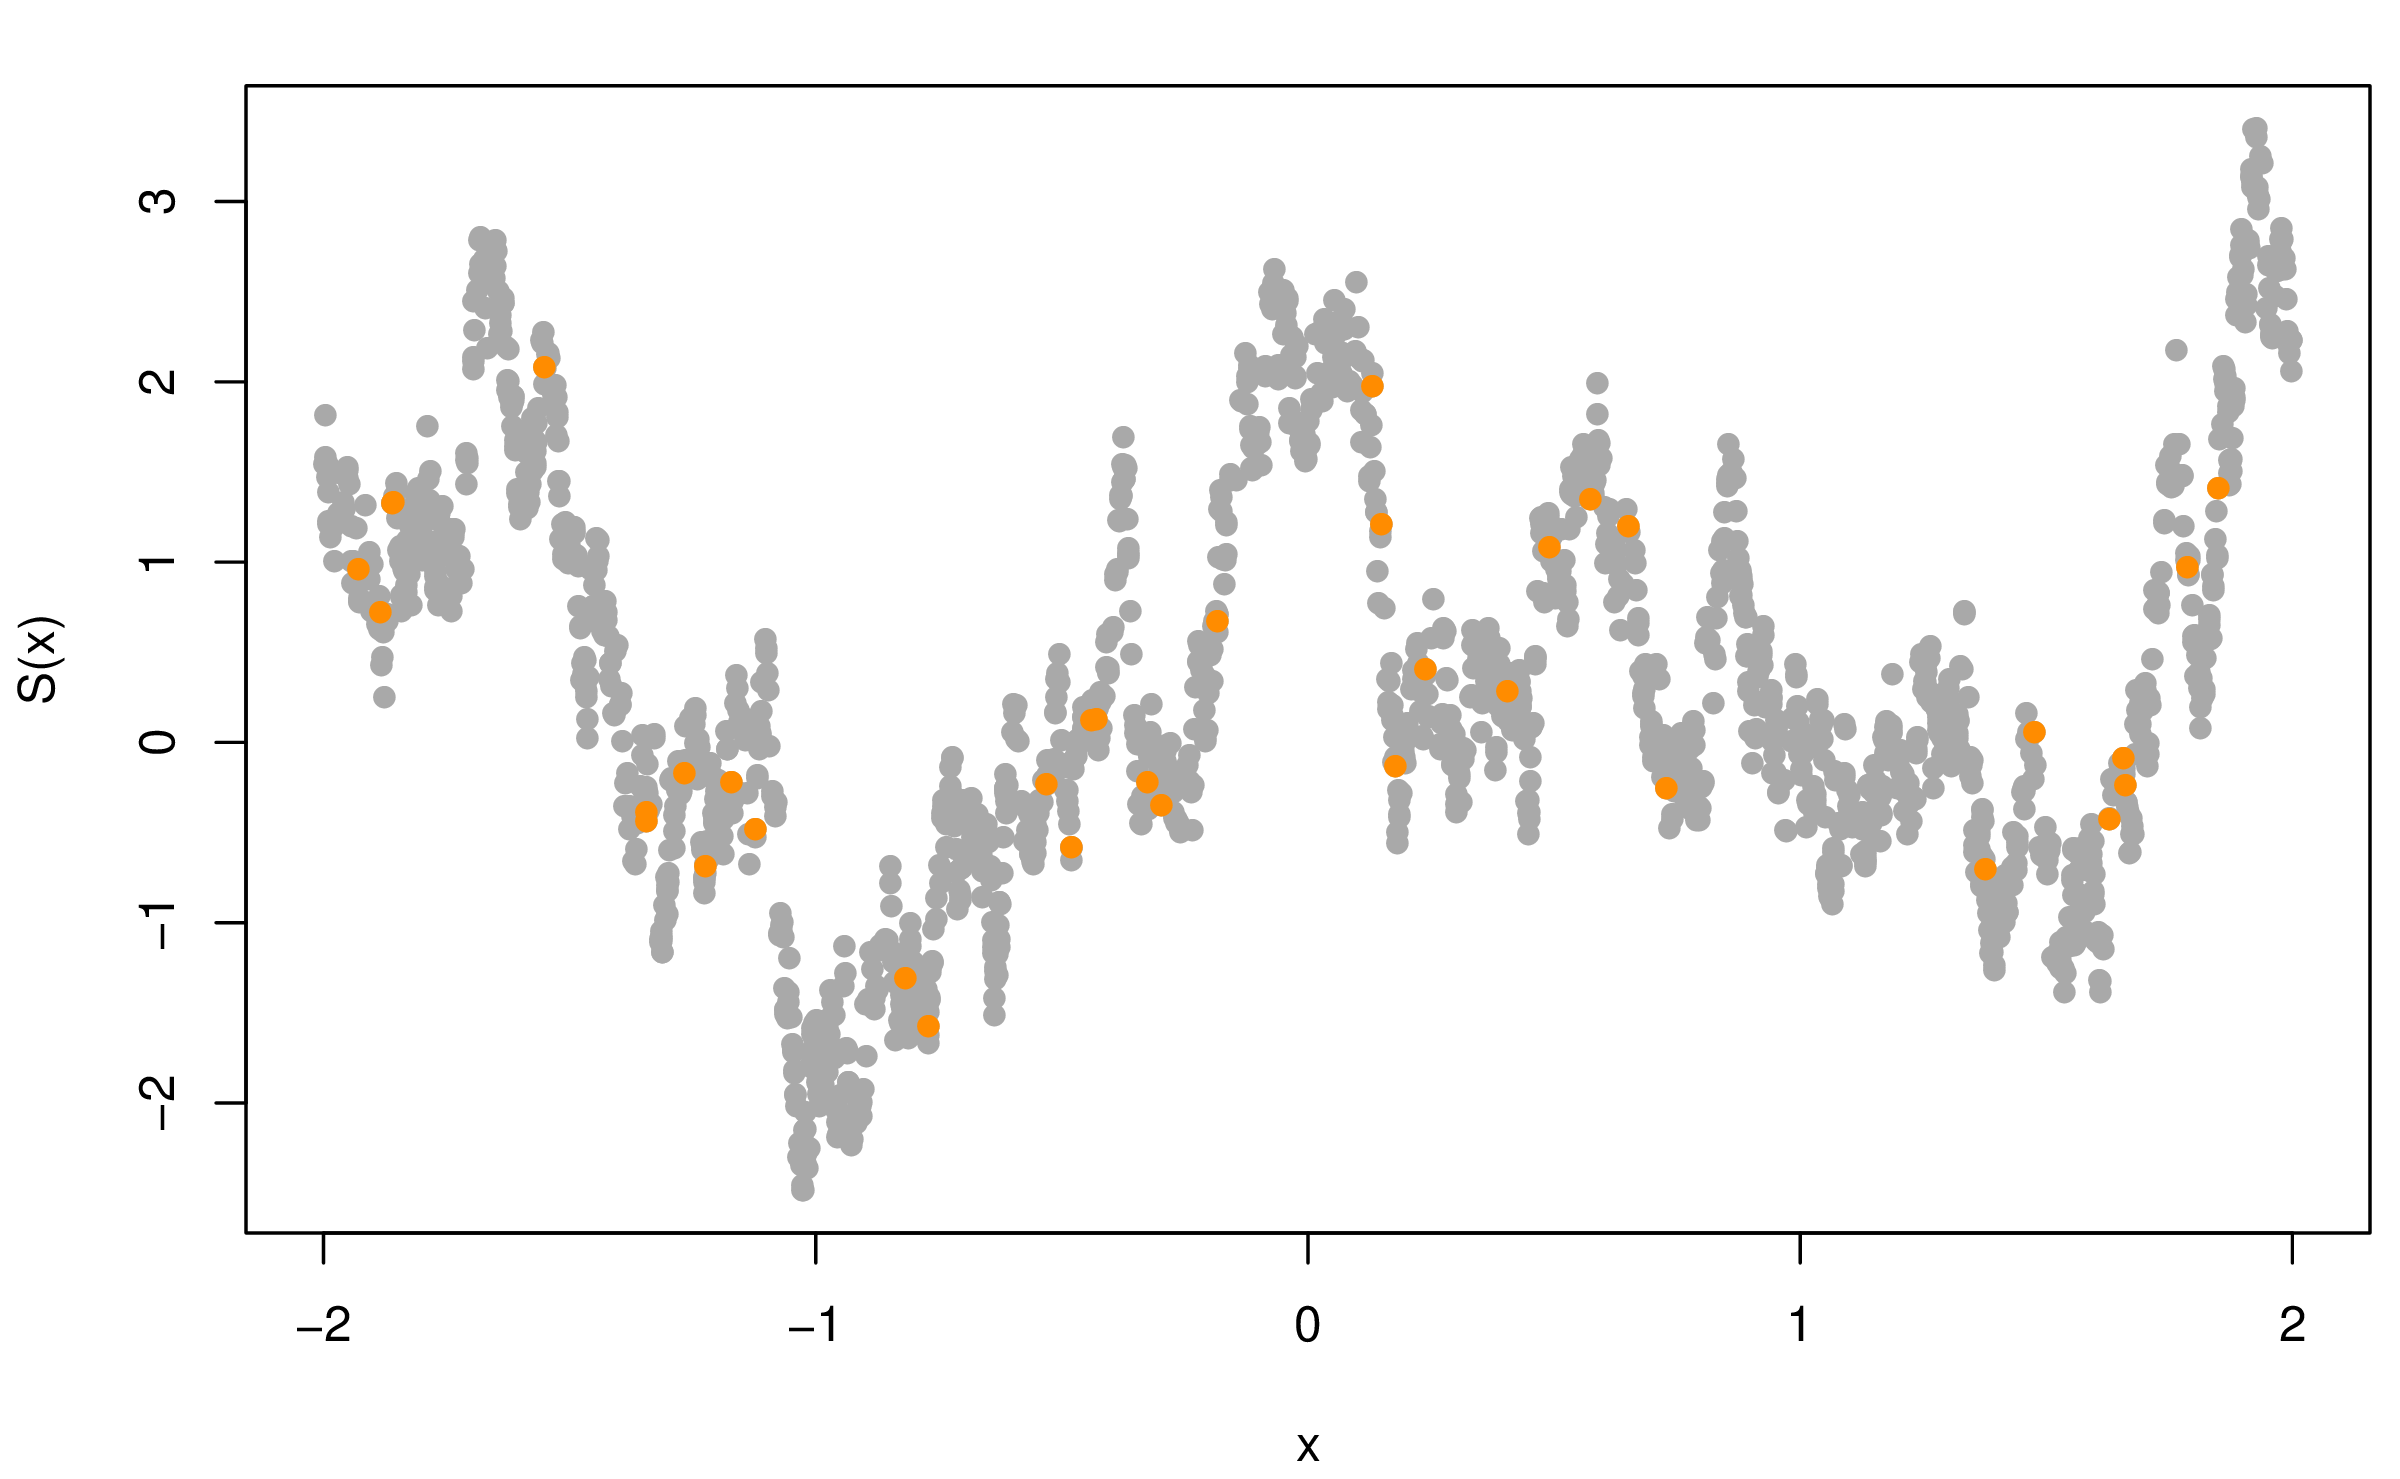
\includegraphics[width=0.7\linewidth]{figures/one-dim-gp-exp} }\\\subfloat[平稳空间高斯过程 $S(x)$ 的协方差函数是幂二次指数型,均值向量为 $\mathbf{0}$,协方差参数 $\sigma^2 = 1$,$\phi = 0.15$,$\kappa=2$\label{fig:one-dim-gp2}]{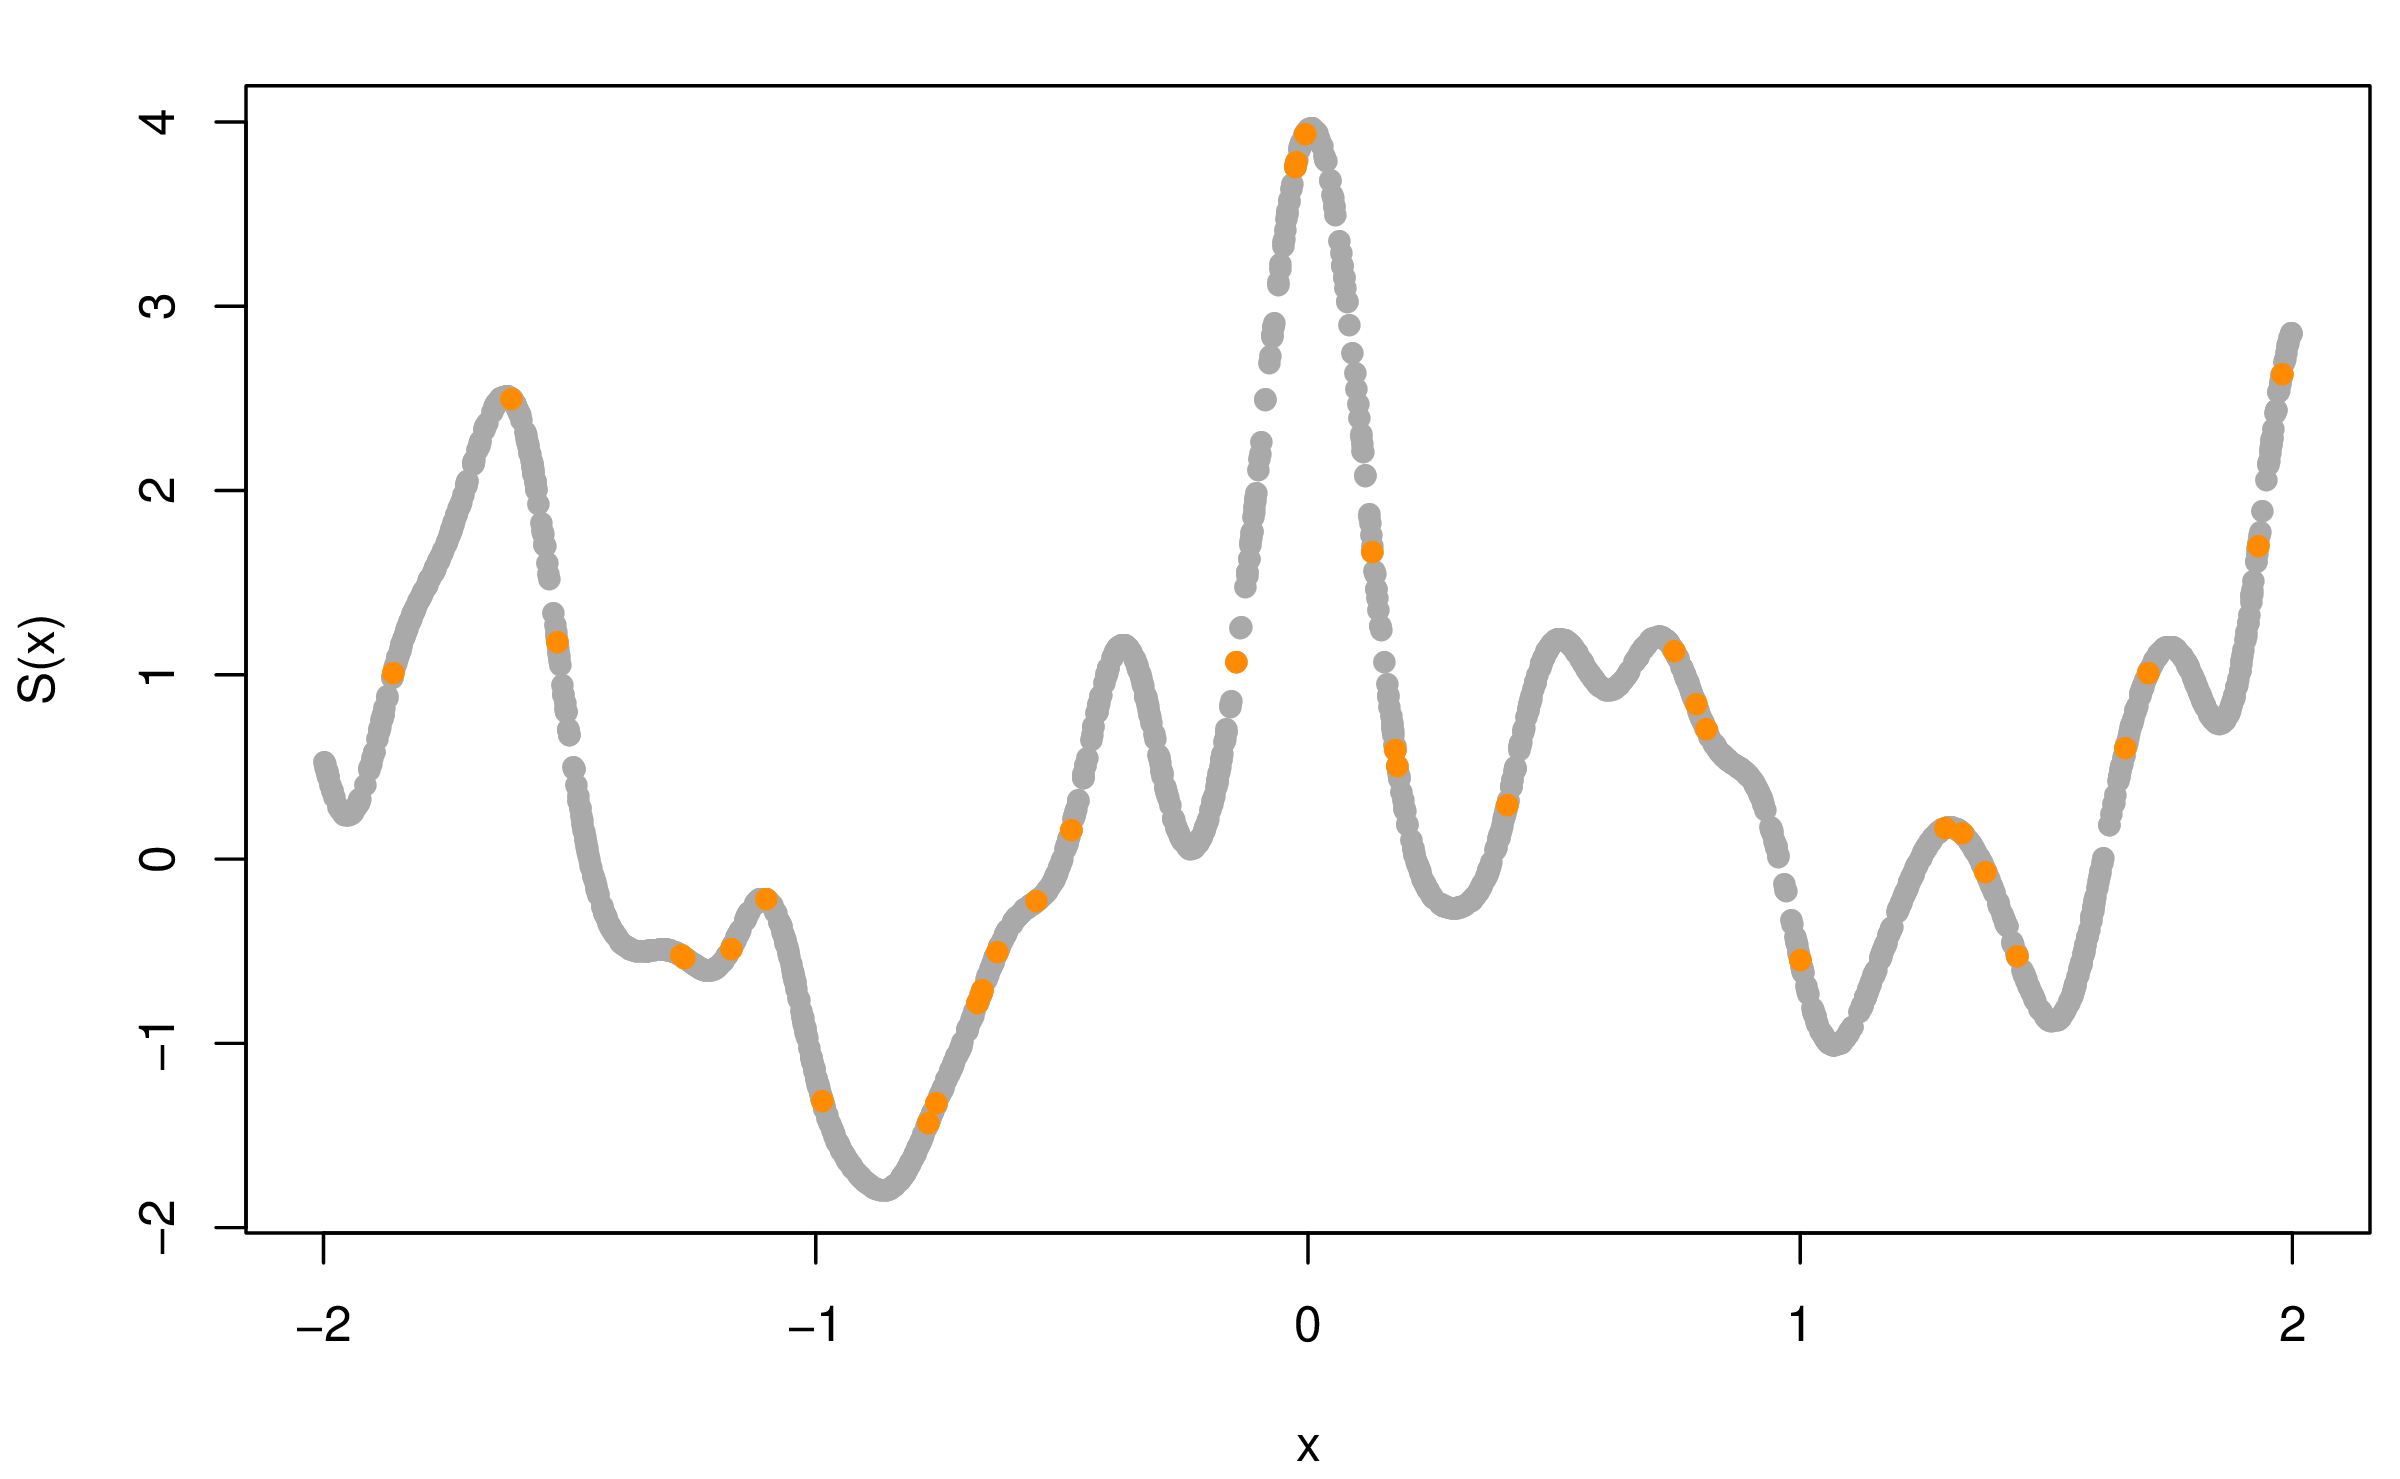
\includegraphics[width=0.7\linewidth]{figures/one-dim-gp-exp-quad} }

}

\caption{模拟一维平稳空间高斯过程,协方差函数分别为指数型
\eqref{eq:cov-exp} 和幂二次指数型 \eqref{eq:cov-exp-quad},均值为
\(\mathbf{0}\),协方差参数
\(\sigma^2 = 1\),\(\phi = 0.15\),横坐标表示采样的位置,纵坐标是目标值
\(S(x)\),图中 2000
个灰色点表示服从相应随机过程的随机数,橘黄色点是从中随机选择的 36 个点。}\label{fig:one-dim-gp}
\end{figure}








根据定理
\ref{thm:stationary-mean-square-properties},指数型协方差函数的平稳高斯过程在原点连续但是不可微,而幂二次指数型协方差函数在原点无穷可微,可微性越好图像上表现越光滑。对比图
\ref{fig:one-dim-gp} 的两个子图, 可以看出,在协方差参数
\(\sigma^2 = 1\),\(\phi = 0.15\) 相同的情况下,\(\kappa\) 越大越光滑。

\hypertarget{sim-two-gp}{%
\subsection{二维平稳空间高斯过程}\label{sim-two-gp}}

二维情形下,在规则平面上模拟平稳高斯过程
\(\mathcal{S} = S(x), x \in \mathbb{R}^2\), 其均值向量为零向量
\(\mathbf{0}\), 协方差函数为指数型,见公式 \eqref{eq:cov-exp},协方差参数
\(\phi = 1, \sigma^2 = 1\)。在单位平面区域为 \([0,1] \times [0,1]\)
模拟服从上述二维平稳空间高斯过程,不妨将此区域划分为 \(6 \times 6\)
的小网格,而每个格点作为采样的位置,共计
36个采样点,在这些采样点上的观察值即为目标值 \(S(x)\)。

类似本章第 \ref{sim-one-gp} 节模拟一维平稳空间过程的步骤,
首先根据采样点位置坐标和协方差函数 \eqref{eq:cov-exp} 计算得目标空间过程的
\(\mathcal{S}\) 协方差矩阵 \(G\),然后使用 R 包 MASS 提供的
\texttt{mvrnorm} 函数产生多元正态分布随机数,与 \ref{sim-one-gp}
节不同的是这里采用特征值分解,即 \(G = L\Lambda L^{\top}\),与 Cholesky
分解相比,特征值分解更稳定些,但是 Cholesky 分解更快,Stan
即采用此法,后续过程与一维模拟一致。模拟获得的随机数用图
\ref{fig:sim-two-gp} 表示, 格点上的值即为平稳空间高斯过程在该点的取值
(为方便显示,已四舍五入保留两位小数)。

\begin{figure}

{\centering \subfloat[在单位区域的网格点上采样\label{fig:sim-two-gp1}]{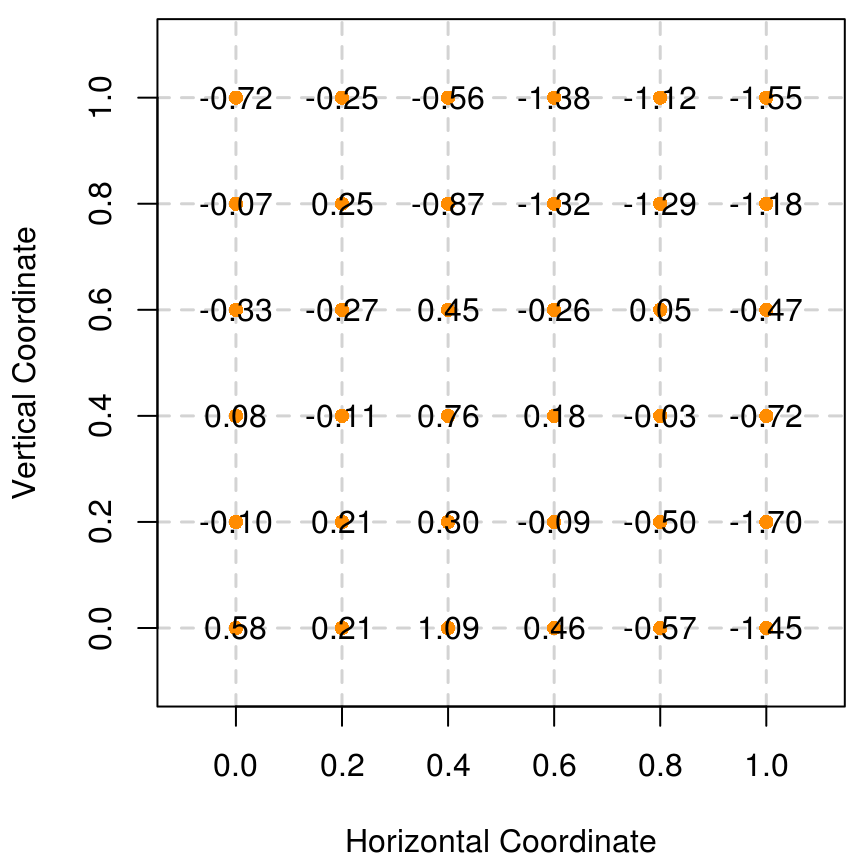
\includegraphics[width=0.45\linewidth]{04-simulations_files/figure-latex/sim-two-gp-1} }\subfloat[在单位区域上随机采样\label{fig:sim-two-gp2}]{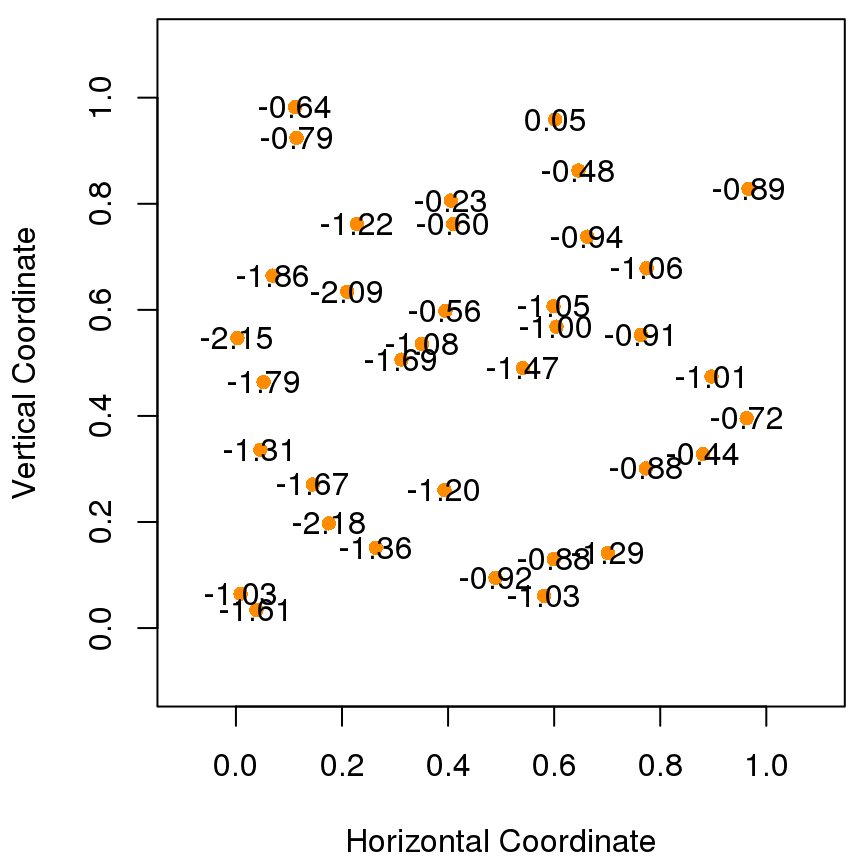
\includegraphics[width=0.45\linewidth]{04-simulations_files/figure-latex/sim-two-gp-2} }

}

\caption{模拟二维平稳空间高斯过程,自相关函数为指数形式,水平方向为横坐标,垂直方向为纵坐标,图中的橘黄色点是采样的位置,其上的数字是目标值 $S(x)$}\label{fig:sim-two-gp}
\end{figure}

同 \ref{sim-one-gp} 节,二维平稳空间高斯过程 \(S(x)\)
的协方差函数也可以为更一般的梅隆型,如公式 \eqref{eq:exp-matern} 所示。
\begin{equation}
\rho(u) = \sigma^2 \{ 2^{\kappa -1} \Gamma(\kappa) \}^{-1}( u/\phi )^{\kappa} \mathcal{K}_{\kappa}( u / \phi ) \label{eq:exp-matern}
\end{equation} \noindent 且在区域 \([0,1] \times [0,1]\)
上也可以随机采点,如图 \ref{fig:sim-two-gp} 的右子图所示。

模拟平稳空间高斯过程的实现方法: Ribeiro 和 Diggle 开发了 geoR 包
\citep{geoR2001},提供的 \texttt{grf} 函数除了实现 Cholesky
分解,还实现了奇异值分解,特征值分解等算法分解协方差矩阵\(G\)。当采样点不太多时,Cholesky
分解已经足够好,下面的第 \ref{sim-sglmm}
节对平稳空间高斯过程的数值模拟即采用此法,当采样点很多,为了加快模拟的速度,可以选用
Schlather 等开发的 RandomFields 包 \citep{RandomFields2015},内置的
\texttt{GaussRF}
函数实现了用高斯马尔科夫随机场近似平稳空间高斯过程的算法,此外,Rue 等
(2009年) \citep{Rue2009}
也实现了从平稳高斯过程到高斯马尔科夫随机场的近似算法,开发了比较高效的
INLA 程序库 \citep{INLA2015},其内置的近似程序得到了一定的应用
\citep{Blangiardo2015, Faraway2018}。

\hypertarget{sim-sglmm}{%
\section{空间广义线性混合效应模型}\label{sim-sglmm}}

\hypertarget{sim-binomal-sglmm}{%
\subsection{响应变量服从二项分布}\label{sim-binomal-sglmm}}

响应变量服从二项分布
\(Y_{i} \sim \mathrm{Binomial}(m_{i},p(x_{i}))\),即在位置 \(x_i\)
处,以概率 \(p(x_i)\) 重复抽取了 \(m_i\) 个样本,总样本数
\(M=\sum_{i=1}^{N}m_i\),\(N\)
是采样点的个数,模拟二项型空间广义线性混合效应模型为
\eqref{eq:binom-SGLMM},联系函数为
\(g(\mu_i) = \log\{\frac{p(x_i)}{1-p(x_i)}\}\),\(S(x)\) 是均值为
\(\mathbf{0}\),协方差函数为
\(\mathsf{Cov}(S(x_i),S(x_j)) = \sigma^2 \big\{2^{\kappa-1}\Gamma(\kappa)\big\}^{-1}(u/\phi)^{\kappa}K_{\kappa}(u/\phi), \kappa = 0.5\)
的平稳空间高斯过程。 \begin{equation}
g(\mu_i) = \log\big\{\frac{p(x_i)}{1-p(x_i)}\big\} = \alpha + S(x_i) \label{eq:binom-SGLMM}
\end{equation} 固定效应参数 \(\alpha = 0\),协方差参数记为
\(\boldsymbol{\theta} = (\sigma^2, \phi) = (0.5, 0.2)\),采样点数目为
\(N = 64\),每个采样点抽取的样本数 \(m_i = 4, i = 1, 2, \ldots, 64\),则
\(Y_i\) 的取值范围为 \(0, 1, 2, 3, 4\)。首先模拟平稳空间高斯过程
\(S(x)\),在单位区域 \([0,1] \times [0,1]\) 划分为 \(8 \times 8\)
的网格,格点选为采样位置,用 geoR 包提供的 \texttt{grf}
函数产生协方差参数为
\(\boldsymbol{\theta} = (\sigma^2,\phi) = (0.5, 0.2)\)
的平稳空间高斯过程,由公式 \eqref{eq:binom-SGLMM} 可知
\(p(x_i) = \exp[\alpha + S(x_i)]/\{1 + \exp[\alpha + S(x_i)]\}\),
即每个格点处二项分布的概率值,然后依此概率,由 \texttt{rbinom}
函数产生服从二项分布的观察值 \(Y_i\),模拟的数据集可以用图
\ref{fig:binom-without-nugget-geoRglm} 直观表示。

\begin{figure}

{\centering 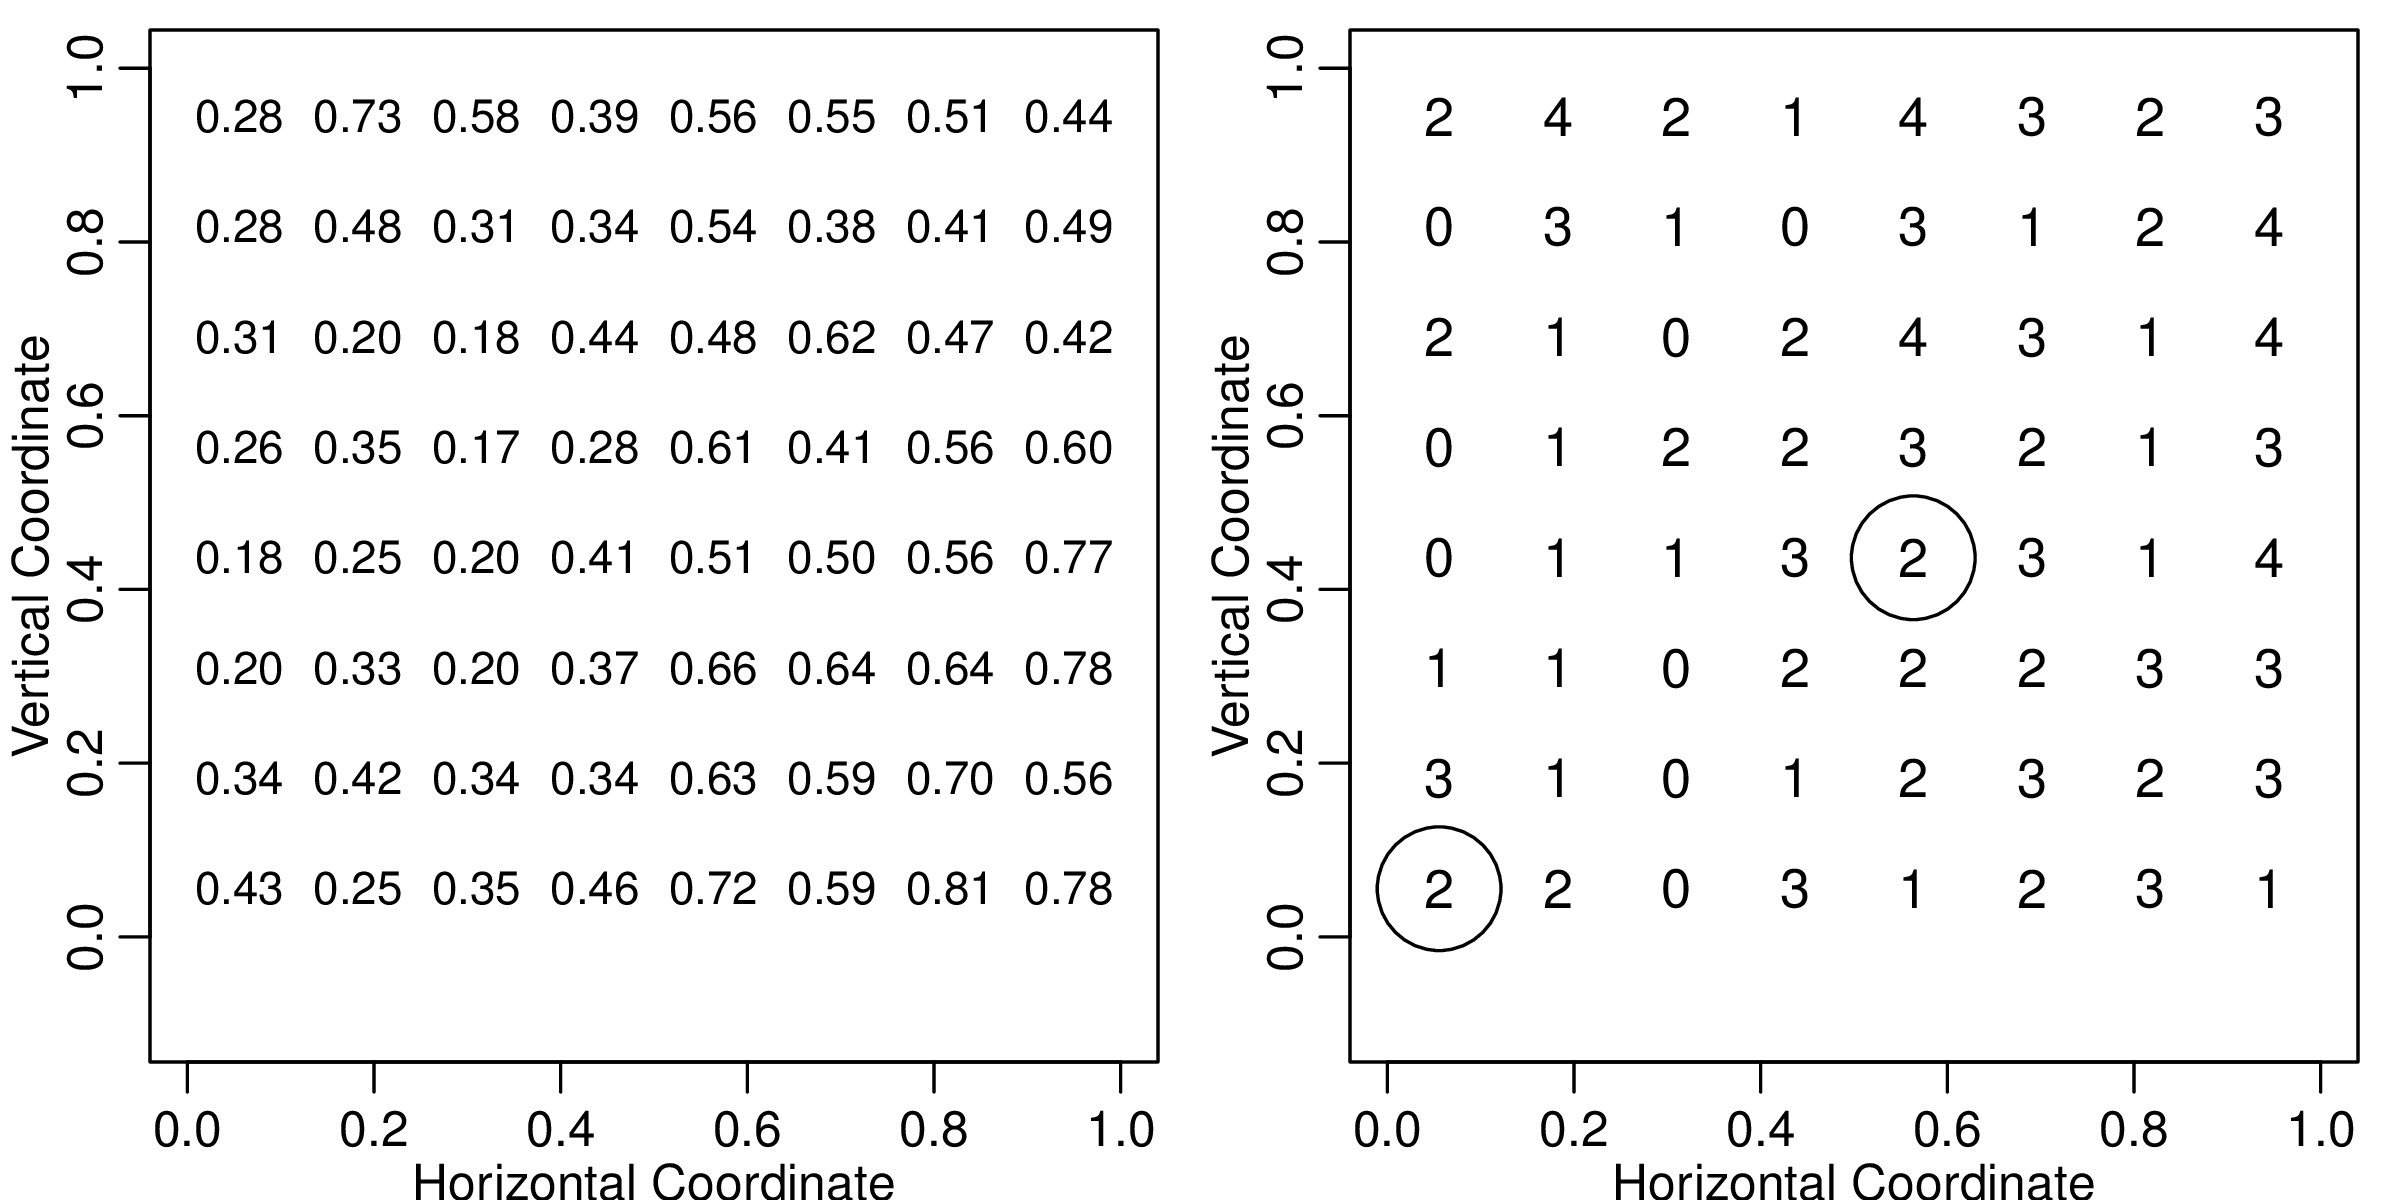
\includegraphics[width=0.9\linewidth]{figures/binom-without-nugget-geoRglm} 

}

\caption{左图表示二维规则平面上的平稳空间高斯过程,格点是采样点的位置,其上的数字是 $p(x)$ 的值,已经四舍五入保留两位小数,右图表示观察值 $Y$ 随空间位置的变化,格点上的值即为观察值 $Y$,图中的两个圈分别是第1个(左下)和第29个(右上)采样点}\label{fig:binom-without-nugget-geoRglm}
\end{figure}

基于 Langevin-Hastings 采样器实现的马尔科夫链蒙特卡罗算法,参数
\(\alpha\) 的先验分布选均值为 0,方差为 1 的标准正态分布,参数 \(\phi\)
的先验分布选期望为 0.2 的指数分布,参数 \(\sigma^2\)
的先验分布是非中心的逆卡方分布(scaled Inverse Chi Square
Distribution),其非中心化参数为 0.5,自由度为 5,各参数的先验选择参考
Christensen 和 Ribeiro (2002年) \citep{geoRglm2002}。Langevin-Hastings
算法运行 110000 次迭代,前 10000 次迭代用作热身 (warm-up),后 10
万次迭代里间隔 100 次迭代采样,获得关于参数 \(\alpha,\phi,\sigma^2\)
的后验分布的样本,样本量是 1000。 \begin{equation}
\alpha \sim \mathcal{N}(0,1), \quad \phi \sim \mathrm{Exp}(0.2), \quad \sigma^2  \sim \mathrm{Inv-}\chi^2(5,0.5)
\end{equation} 参数 \(\alpha,\phi,\sigma^2\)
的贝叶斯估计没有显式表达式,通常以 MCMC
算法获得后验分布的样本均值作为参数的估计。贝叶斯估计的定义是使得估计的均方误差达到最小时的估计,因此贝叶斯估计的精度或者说好坏常用后验分布的方差衡量,因为均方误差在参数估计取后验均值时是后验方差,故而表
\ref{tab:MCLH-vs-NUTS} 不再提供估计的均方误差值,而是提供了 5
个后验分布的分位点,在 95\% 的置信水平下,样本分位点 0.025 和 0.975
的值组成了置信区间的上下界。除了获得各参数的估计值外,还获得 64
个采样点处 \(p(x_i), i = 1, \ldots, 64\) 的后验均值、方差、标准差和
5个分位点,详见附表 \ref{tab:LH-binom-SGLMM}。

\begin{longtable}[]{@{}lrrrrrrrrrr@{}}
\caption{\label{tab:MCLH-vs-NUTS} Langevin-Hastings 算法与 HMC
算法的数值模拟比较,前者在R软件里基于 geoRglm 包实现,后者基于 Stan
实现。表格中的列依次是模型参数 \(\alpha,\phi,\sigma^2\)
的真值、后验均值、后验方差、后验的
5个分位点和样本量\(N\)。采样点数目分别考虑了 \(N = 36, 64, 81\)
的情况,对于每组参数设置,重复模拟了100 次,表格前半部分是
Langevin-Hastings 算法得到的结果,后半部分是 HMC
算法得到的结果}\tabularnewline
\toprule
& true(init) & mean & var & 2.5\% & 25\% & 50\% & 75\% & 97.5\% & N &
time(s)\tabularnewline
\midrule
\endfirsthead
\toprule
& true(init) & mean & var & 2.5\% & 25\% & 50\% & 75\% & 97.5\% & N &
time(s)\tabularnewline
\midrule
\endhead
\(\alpha\) & 0.0(0.387) & -0.354 & 0.079 & -0.938 & -0.524 & -0.361 &
-0.173 & 0.215 & 36 & 600.12\tabularnewline
\(\phi\) & 0.2(0.205) & 0.121 & 0.006 & 0.005 & 0.055 & 0.110 & 0.180 &
0.285 & &\tabularnewline
\(\sigma^2\) & 0.5(1.121) & 0.683 & 0.147 & 0.215 & 0.408 & 0.596 &
0.850 & 1.667 & &\tabularnewline
\(\alpha\) & 0.0(0.157) & 0.003 & 0.089 & -0.596 & -0.169 & 0.013 &
0.179 & 0.609 & 64 & 729.19\tabularnewline
\(\phi\) & 0.2(0.110) & 0.194 & 0.004 & 0.070 & 0.145 & 0.195 & 0.250 &
0.295 & &\tabularnewline
\(\sigma^2\) & 0.5(0.494) & 0.656 & 0.096 & 0.254 & 0.449 & 0.592 &
0.781 & 1.453 & &\tabularnewline
\(\beta\) & 0.0(-0.006) & -0.155 & 0.044 & -0.565 & -0.284 & -0.156 &
-0.03 & 0.273 & 81 & 844.56\tabularnewline
\(\phi\) & 0.2(0.185) & 0.116 & 0.006 & 0.005 & 0.055 & 0.105 & 0.17 &
0.280 & &\tabularnewline
\(\sigma^2\) & 0.5(0.403) & 0.468 & 0.057 & 0.180 & 0.311 & 0.414 & 0.56
& 1.129 & &\tabularnewline
\(\alpha\) & 0.0(-0.813) & -0.230 & 0.209 & -1.127 & -0.521 & -0.214 &
0.056 & 0.653 & 36 & 6.65\tabularnewline
\(\phi\) & 0.2(1.692) & 1.103 & 0.364 & 0.459 & 0.721 & 0.936 & 1.284 &
2.669 & &\tabularnewline
\(\sigma^2\) & 0.5(0.144) & 0.474 & 0.187 & 0.105 & 0.216 & 0.333 &
0.573 & 1.572 & &\tabularnewline
\(\alpha\) & 0.0(0.155) & 0.046 & 0.251 & -0.947 & -0.269 & 0.049 &
0.356 & 1.069 & 64 & 27.70\tabularnewline
\(\phi\) & 0.2(1.766) & 1.042 & 0.246 & 0.471 & 0.708 & 0.921 & 1.247 &
2.324 & &\tabularnewline
\(\sigma^2\) & 0.5(0.808) & 0.647 & 0.228 & 0.170 & 0.338 & 0.524 &
0.779 & 1.958 & &\tabularnewline
\(\alpha\) & 0.0(-0.369) & -0.082 & 0.170 & -0.893 & -0.321 & -0.078 &
0.174 & 0.742 & 81 & 45.69\tabularnewline
\(\phi\) & 0.2(0.911) & 1.110 & 0.331 & 0.453 & 0.721 & 0.986 & 1.330 &
2.506 & &\tabularnewline
\(\sigma^2\) & 0.5(0.302) & 0.410 & 0.105 & 0.105 & 0.205 & 0.317 &
0.503 & 1.211 & &\tabularnewline
\bottomrule
\end{longtable}

为了获得尽量好的效果,在样本量 \(N = 64\) 时,花了近三天时间反复调了
Langevin-Hastings
算法的参数,相比较而言,得到了一组非常好的结果。然而,当改变样本量时,考虑到又需要漫长的调参,对样本量是36和81时,只要求迭代序列保持收敛即可。基于
Stan 实现的 HMC
算法没有调参数,初值和先验分布也采用默认的,总迭代次数设为2000次,前1000次迭代作为热身阶段(warm-up),后1000次的迭代值全部采样,所有的迭代序列都通过了平稳性检验。

根据模拟的过程和表\ref{tab:MCLH-vs-NUTS}的结果来看,基于 Stan 实现的 HMC
算法更易收敛,且对初始值和先验分布相对不那么敏感,不需要耗时的调参过程。表
\ref{tab:MCLH-vs-NUTS} 中 Langevin-Hastings 算法的时间由 R 内置的函数
\texttt{system.time()} 记录。初始值是 burn-in 的位置,即完成 warm-up
阶段后,开始采样的第一个迭代点。

\hypertarget{possion-sglmm}{%
\subsection{响应变量服从泊松分布}\label{possion-sglmm}}

模拟响应变量 \(Y\) 服从泊松分布,即
\(Y_i \sim \mathrm{Poisson}(\lambda(x_{i}))\)
的泊松型空间广义线性混合效应模型 \begin{equation}
g(\mu_i) = \log[\lambda(x_i)] = \alpha + S(x_i) \label{eq:pois-SGLMM}
\end{equation} \noindent 其中,\(S(x)\) 是平稳空间高斯过程,其均值为
\(\mathbf{0}\),协方差函数为
\(\mathrm{Cov}(S(x_i),S(x_j)) = \sigma^2 \big\{2^{\kappa-1}\Gamma(\kappa)\big\}^{-1}(u/\phi)^{\kappa}K_{\kappa}(u/\phi)\),联系函数
\(g(\mu_i) = \log[\lambda(x_{i})]\)。

类似 \ref{sim-binomal-sglmm} 小节,首先产生服从平稳空间高斯过程 \(S(x)\)
的随机数 \(S(x_i),i=1,\ldots,N\),然后由 \eqref{eq:pois-SGLMM} 式可得
\(\lambda(x_i) = \exp(\alpha + S(x_i))\),且响应变量
\(Y_i \sim \mathrm{Poisson}(\lambda(x_{i}))\),根据 R 内置函数
\texttt{rpois} 即可 产生服从参数为 \(\lambda(x_i)\)
的泊松分布的随机数。Langevin-Hastings 算法和 HMC 算法模拟的结果见表
\ref{tab:Pois-MCLV-vs-NUTS}。HMC 算法包含有效样本数 \(n_{eff}\)、
潜在尺度缩减因子 \(\hat{R}\) 和蒙特卡罗均值误差 se\_mean
的完整表格见附表
\ref{tab:HMC-Pois-SGLMM},参数迭代序列的收敛性分析已在第\ref{prepare}
章第\ref{sec:stan-samplers}节给出,这里不再赘述,所有的模拟实验都是在完成收敛性分析后给出的。

\begin{longtable}[]{@{}lrrrrrrrrrr@{}}
\caption{\label{tab:Pois-MCLV-vs-NUTS}
在模型\eqref{eq:pois-SGLMM}的设置下,Langevin-Hastings 算法和 HMC
算法的比较,模型参数真值设置为
\(\alpha = 0.5, \phi = 0.2, \sigma^2 = 2.0, \kappa = 1.5\),采样点数目分别为
\(N=36,64,100\),对于每组参数设置,重复模拟了100次。表格各列依次是参数的真值、后验均值、后验方差、后验五个分位点和样本量。表格前半部分是
Langevin-Hastings 算法实现的结果,后半部分是 Stan
实现的结果}\tabularnewline
\toprule
& true(init) & mean & var & 2.5\% & 25\% & 50\% & 75\% & 97.5\% & N &
time(s)\tabularnewline
\midrule
\endfirsthead
\toprule
& true(init) & mean & var & 2.5\% & 25\% & 50\% & 75\% & 97.5\% & N &
time(s)\tabularnewline
\midrule
\endhead
\(\alpha\) & 0.5(1.201) & 0.527 & 0.418 & -0.759 & 0.189 & 0.514 & 0.855
& 1.864 & 36 & 642.66\tabularnewline
\(\phi\) & 0.2(0.420) & 0.401 & 0.052 & 0.100 & 0.240 & 0.360 & 0.520 &
0.960 & &\tabularnewline
\(\sigma^2\) & 2.0(1.038) & 1.311 & 0.660 & 0.365 & 0.766 & 1.081 &
1.584 & 3.562 & &\tabularnewline
\(\alpha\) & 0.5(1.211) & 0.866 & 1.517 & -1.610 & 0.059 & 0.870 & 1.666
& 3.159 & 64 & 883.76\tabularnewline
\(\phi\) & 0.2(0.480) & 0.682 & 0.073 & 0.300 & 0.480 & 0.640 & 0.820 &
1.380 & &\tabularnewline
\(\sigma^2\) & 2.0(2.232) & 3.932 & 2.594 & 1.667 & 2.800 & 3.642 &
4.744 & 7.740 & &\tabularnewline
\(\alpha\) & 0.5(0.189) & 0.323 & 0.657 & -1.449 & -0.124 & 0.416 &
0.812 & 1.831 & 100 & 1223.28\tabularnewline
\(\phi\) & 0.2(0.540) & 0.617 & 0.085 & 0.220 & 0.400 & 0.560 & 0.785 &
1.320 & &\tabularnewline
\(\sigma^2\) & 2.0(1.395) & 1.479 & 0.498 & 0.545 & 0.941 & 1.352 &
1.822 & 3.195 & &\tabularnewline
\(\alpha\) & 0.5(0.335) & 0.483 & 0.310 & -0.608 & 0.094 & 0.488 & 0.851
& 1.613 & 36 & 11.25\tabularnewline
\(\phi\) & 0.2(0.066) & 0.631 & 0.036 & 0.362 & 0.501 & 0.602 & 0.722 &
1.090 & &\tabularnewline
\(\sigma^2\) & 2.0(0.347) & 1.370 & 0.298 & 0.455 & 0.977 & 1.317 &
1.714 & 2.566 & &\tabularnewline
\(\alpha\) & 0.5(1.021) & 0.498 & 0.402 & -0.775 & 0.082 & 0.534 & 0.917
& 1.798 & 64 & 113.04\tabularnewline
\(\phi\) & 0.2(0.370) & 0.385 & 0.003 & 0.285 & 0.343 & 0.380 & 0.422 &
0.509 & &\tabularnewline
\(\sigma^2\) & 2.0(2.610) & 2.473 & 0.292 & 1.585 & 2.102 & 2.416 &
2.804 & 3.734 & &\tabularnewline
\(\alpha\) & 0.5(0.613) & 0.400 & 0.297 & -0.723 & 0.062 & 0.415 & 0.767
& 1.412 & 100 & 272.58\tabularnewline
\(\phi\) & 0.2(0.294) & 0.299 & 0.005 & 0.181 & 0.243 & 0.289 & 0.343 &
0.465 & &\tabularnewline
\(\sigma^2\) & 2.0(1.724) & 1.146 & 0.206 & 0.525 & 0.824 & 1.037 &
1.395 & 2.282 & &\tabularnewline
\bottomrule
\end{longtable}

100 个采样点的模拟实验中,不断试错调了 Langevin-Hastings
算法的参数,得到比较好的估计值,在该组参数设置下,更改采样点数目分别为
36 和 64,又需要重新调整 Langevin-Hastings
算法的参数设置,以获得参数的后验分布和后续的后验量的计算。

在同组参数设置下,基于 Stan 实现的 HMC 算法与 Langevin-Hastings
算法相比,效果要好,其一体现在后验方差更小,也是贝叶斯估计下的均方误差更小,见表
\ref{tab:Pois-MCLV-vs-NUTS};其二对于应用的意义更大,它不需要调参数,对先验分布的要求更加宽松;其三算法收敛的更快,基于
Langevin-Hastings 算法实现的贝叶斯 MCMC
算法迭代次数设置为110000,前10000次迭代作为 warm-up,间隔 100
次迭代采样,收集到的样本量是 1000,基于 Stan 实现的 HMC 算法只进行了
2000 次迭代,前 1000 次迭代作为 warm-up 阶段,后 1000
次迭代全部采样,所以样本量也是
1000。这里需要补充说明一下,比较两个算法却在迭代次数上做了不同的设置,是因为首先要保证模型参数的迭代序列要收敛,只有这样才能作参数的后验估计,那么同样达到收敛状态,Langevin-Hastings
算法大约110000次迭代,而基于 Stan 实现的 HMC 算法大于 2000
次迭代,如果强行继续增加后者算法的迭代次数是意义不大的,因为它已经收敛,增加迭代次数只会无端添加算法运行时间。

\hypertarget{sec:simulations}{%
\section{本章小结}\label{sec:simulations}}

geoRglm 包实现的 Langevin-Hastings
算法,相比较而言,收敛速度慢,迭代序列自相关性表现拖尾,因此在上述模拟实验中,为了降低相关性,采样间隔取100,这就直接要求增加总的迭代次数以达到足够的后验样本量,这样才能用于后验量的计算。此外,在调参数的过程中面临不收敛的情况是常有的,而这个不收敛的原因至少有两个,其一是参数初值不合适,其二是总迭代次数不够。因此,我们也遭遇了
Christensen
迭代上百万次的\href{http://gbi.agrsci.dk/~ofch/geoRglm/Intro/books.html}{情形},在尽量保持统一的参数设置下,我们选择继续调整参数,而保持总迭代次数110000次不变。在每组模型设置下都获得最佳的参数,这无疑是一件十分耗时的工作,因为该算法的参数只有不断试错才能获得更加合适的参数设置,特别地,在已经收敛的情形下,再去调参数,这个过程会更加漫长。

基于 Stan 实现的贝叶斯 STAN-MCMC 算法,其内置的 HMC 算法是结合了 NUTS
采样器\citep{hoffman2014},搜索模型参数的策略更加友好,不需要手动调参数,只需要指定合适的参数先验,使得迭代序列保持收敛即可,编程过程中,模型参数的重参数化(reparameterization)对迭代进程和结果会产生一定影响,如第\ref{prepare}章第\ref{sec:stan-samplers}节基于
Eight Schools 数据集介绍分层正态模型就对参数 \(\mu\) 和 \(\sigma\)
做了重参数化。

基于似然推断的算法,如第\ref{algorithms}章第\ref{subsec:MCML}小节介绍的蒙特卡罗极大似然算法和第\ref{subsec:LA}小节介绍的拉普拉斯近似算法,都需要非常接近真值的参数初值,才能得到好的结果,因为在大多数情形下,SGLMM
模型的对数似然曲面是呈现山岭或峡谷状,局部极值点多而且对数似然函数值变化不大,导致收敛速度极慢或者陷入局部极值点的收敛,非常难获得全局极值点。因此,一个合适的策略是在合理的初值周围打网格,格点作为迭代初值,以不同的初值进行迭代,将计算的剖面似然函数轮廓画在二维平面上,通过这种降维观察的方式,获得一个可靠的全局极值点,作为参数的最佳似然估计,在后续的第\ref{applications}章第\ref{case-rongelap}节以分析朗格拉普岛核污染数据集为例,介绍这一策略。

\hypertarget{applications}{%
\chapter{数据分析}\label{applications}}

第\ref{sec:spatial-random-effects}节基于小麦产量数据建立空间线性混合效应模型,以
R 软件和相关 R
包为工具,介绍空间统计建模分析的过程,特别是诊断和添加空间随机效应的分析方法和模型参数初值的确定方式。这个分析方法和初值的确定方式具有普适性,对于更复杂的空间广义线性混合效应模型也是适用的。第\ref{case-rongelap}节建立响应变量服从泊松分布的空间广义线性混合效应模型分析一个真实数据集
rongelap。rongelap 数据集目前由 Christensen 维护在 R 包 geoRglm 里,曾被
Diggle 等 (1998年) \citep{Diggle1998} 、Christensen (2004年)
\citep{Christensen2004} 和 Ribeiro 和 Bonat (2016年)
\citep{Bonat2016Practical} 分析过,第 \ref{case-rongelap}
节首先分别基于第\ref{algorithms}章第\ref{subsec:MCML}小节介绍的蒙特卡罗极大似然算法和第\ref{subsec:LA}小节介绍的拉普拉斯近似算法估计泊松型空间广义线性混合效应模型的参数,与他们不同的是,这里进一步根据不同的初始值观察迭代陷入局部极值点或者由于似然曲面太平坦致使迭代终止的情况,因此提出结合第\ref{algorithms}章第\ref{sec:profile-likelihood}节介绍的剖面似然函数的想法,借助剖面似然函数轮廓来确定更加合适的初值。

\hypertarget{sec:spatial-random-effects}{%
\section{小麦产量的空间分布}\label{sec:spatial-random-effects}}

Stroup 和 Baenziger (1994年) \citep{Stroup1994}
采用完全随机的区组设计研究小麦产量与品种等因素的关系,在 4
块肥力不同的地里都随机种植了 56 种不同的小麦,
实验记录了小麦产量、品种、位置以及土地肥力等数据, Pinheiro 和 Bates
(2000年) \citep{Pinheiro2000} 将该数据集命名为 Wheat2 ,整理后放在
nlme 包里。
这里利用该真实的农业生产数据构建带空间效应的线性混合效应模型,详述选初值、诊断和添加空间效应的过程。

\begin{figure}

{\centering 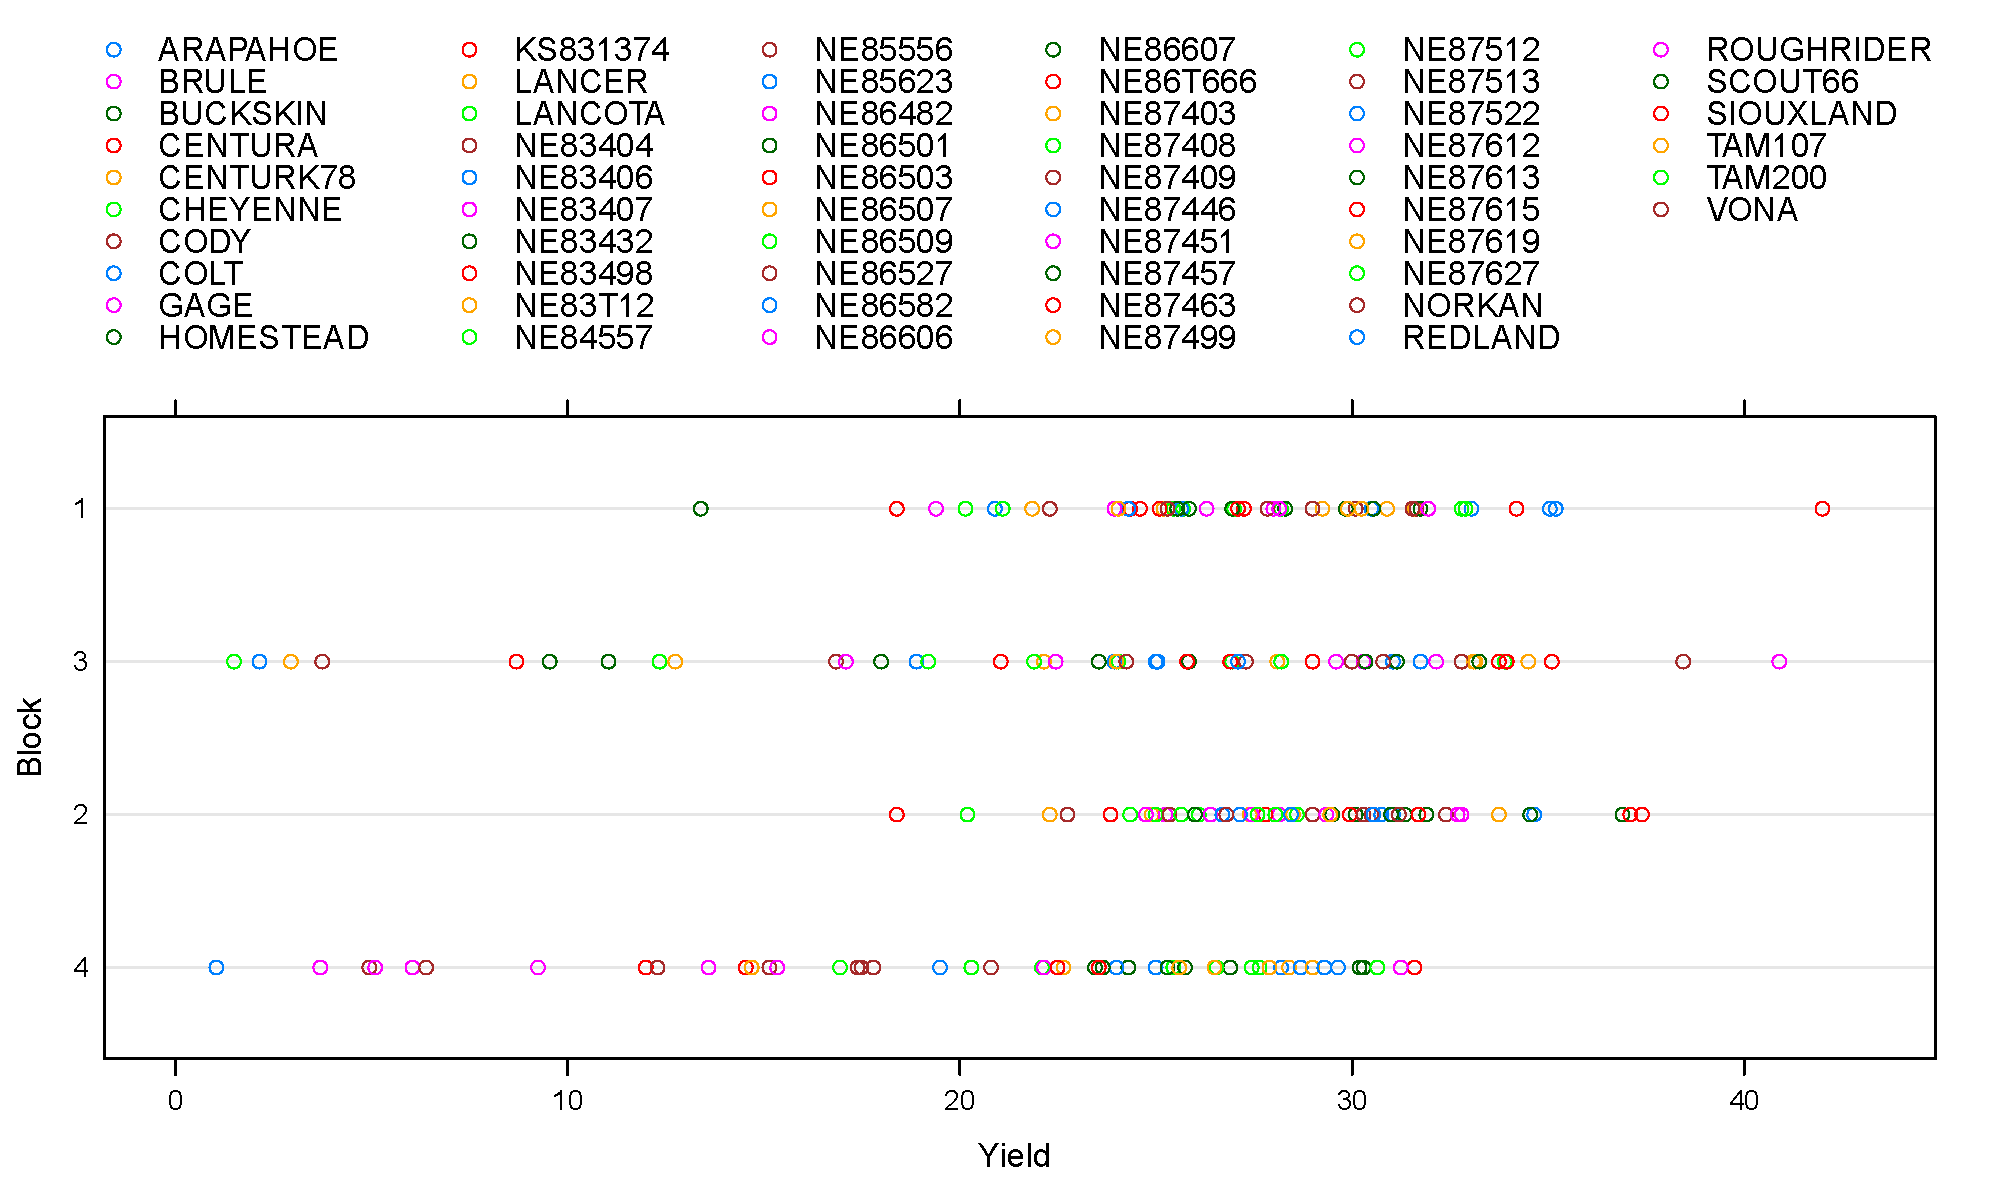
\includegraphics[width=0.7\linewidth]{figures/Yields-Block} 

}

\caption{小麦产量与土壤肥力的关系,图中纵轴表示试验田的4种类型,且土壤肥力强弱顺序是 1 > 2 > 3 > 4,横轴表示小麦产量,每块试验田都种植了 56 种小麦,图中分别以不同的颜色标识,图上方是小麦类型的编号}\label{fig:yields-block}
\end{figure}

图 \ref{fig:yields-block}
按土壤肥力不同分块展示每种小麦的产量,图中暗示数据中有明显的 block
效应,即不同实验田对结果产生显著影响,而且不同实验田之间,小麦产量呈现异方差性,为了更好地表达这些效应,可以基于经纬度坐标信息添加与空间相关的结构
(spatial correlation structures)。基于上述对图\ref{fig:yields-block}
的探索,先建立一般的线性模型,以量化上述描述性分析结果,模型结构如下
\begin{equation}
y_{ij} = \tau_i + \epsilon_{ij}, \quad \boldsymbol{\epsilon} \sim \mathcal{N}(\mathbf{0},\sigma^2 \boldsymbol{\Lambda}) \label{eq:extended-linear-model}
\end{equation} \noindent 其中,\(y_{ij}\) 表示第 \(i\) 种小麦在第 \(j\)
块试验田里的产量,\(i = 1,\ldots,56\),\(j = 1,\ldots,4\)。 \(\tau_i\)
表示第 \(i\) 种小麦的平均产量,\(\epsilon_{ij}\)
是随机误差,假定服从均值为 0,协差阵为 \(\sigma^2 \boldsymbol{\Lambda}\)
的多元正态分布。进一步,继续探索线性模型\eqref{eq:extended-linear-model}中的协方差
\(\boldsymbol{\Lambda}\) 的结构,不妨先假定模型
\eqref{eq:extended-linear-model} 的随机误差是独立且方差齐性的,即
\(\boldsymbol{\Lambda} = \boldsymbol{I}\)
。接着,需要确认方差齐性的假设是否合适,拟合残差散点图是一个有用又方便的判断工具。特别地,对于空间效应的探索,采用样本变差图探索数据中存在的空间相关性,可调用
nlme 包中的 \texttt{Variogram} 函数获得 \texttt{gls}
函数拟合方差齐性的线性模型的变差图\ref{fig:yields-variogram}。

\begin{figure}

{\centering 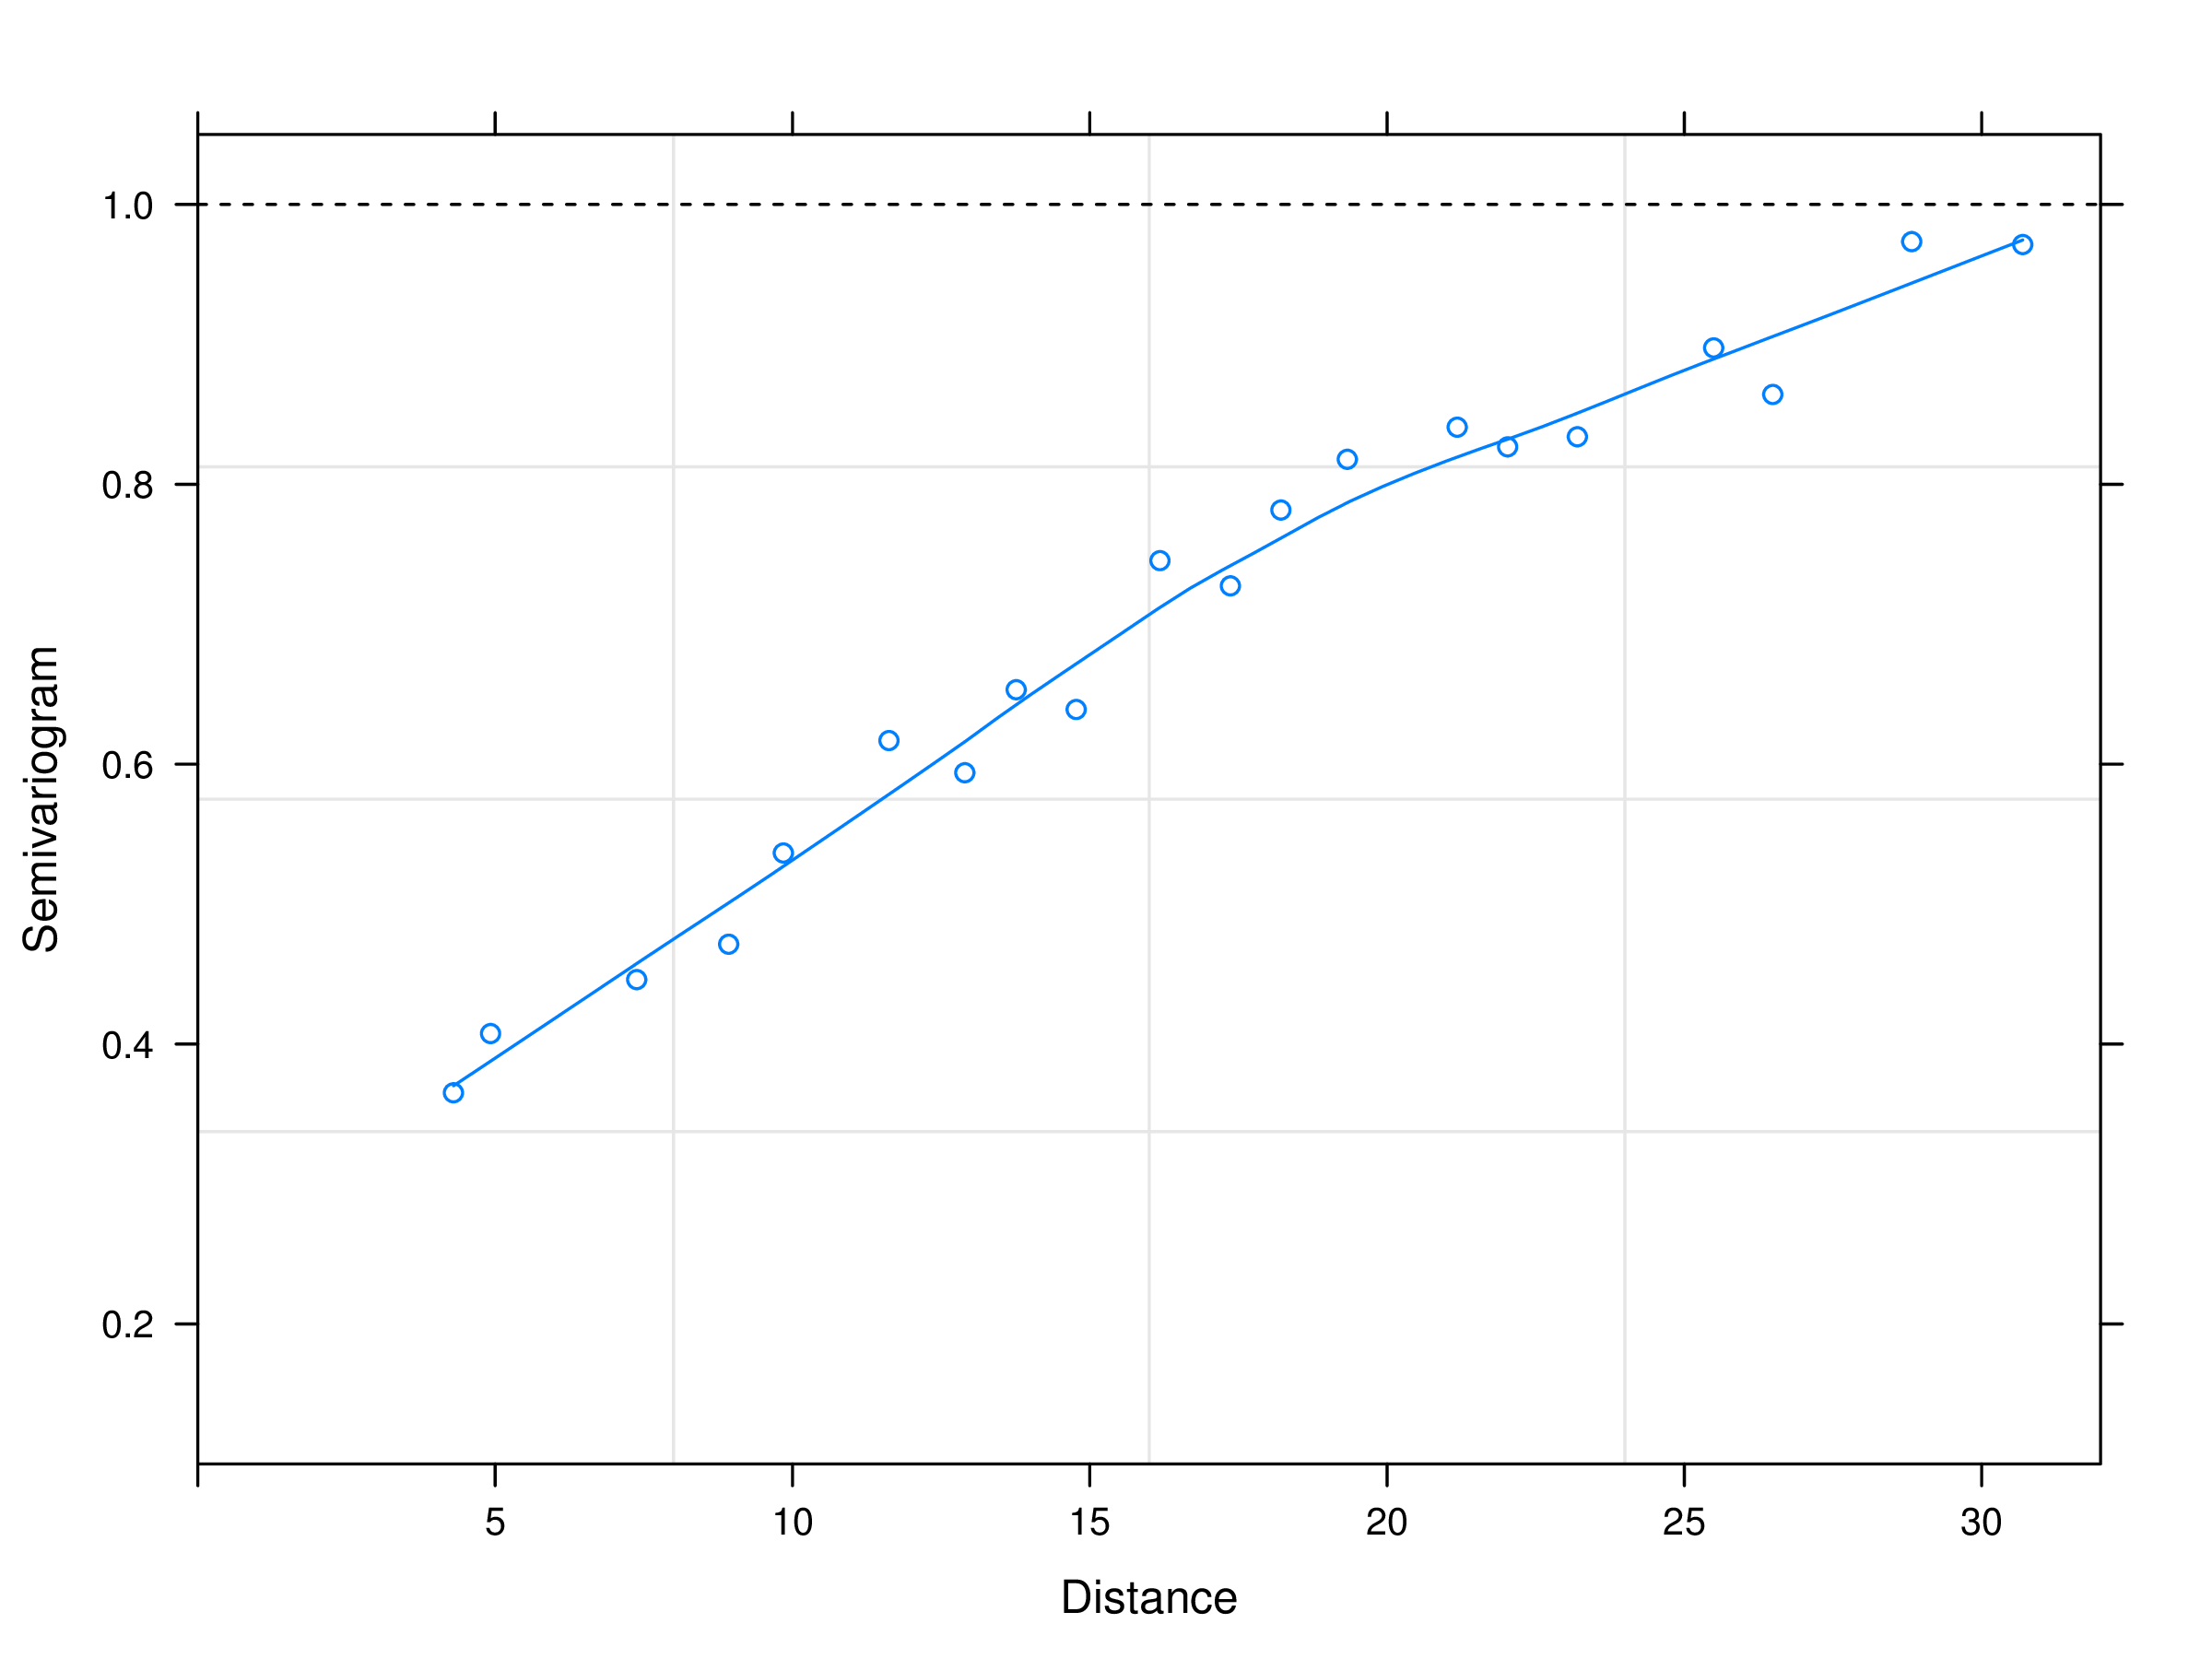
\includegraphics[width=0.7\linewidth]{figures/Yields-Variogram} 

}

\caption{样本变差散点图,横坐标是小麦之间的欧氏距离,纵坐标是样本变差,图中的平滑线根据局部多项式拟合的方法添加,用以估计样本变差的大致趋势}\label{fig:yields-variogram}
\end{figure}

图 \ref{fig:yields-variogram}
显示样本变差随空间距离有明显的增长趋势,可见空间随机效应明显,根据第\ref{models}章第\ref{subsec:covariance-function}小节,可以有理由地估计块金效应\(\tau^2\)大约是
0.2,参数 \(\phi\) 可由样本变差为 1
对应的空间距离来初步估计,图\ref{fig:yields-variogram}显示该值大约是
31。 图中的平滑曲线是
局部多项式回归拟合的结果,也可以用局部加权回归拟合的平滑法来确定初值
\citep{Xie2008COS}。上述图示分析,首先采用球性自相关函数拟合这组数据中的空间结构。考虑空间效应后,采用
\texttt{gls} 函数提供的限制极大似然法 (Restricted Maximum Likelihood
Estimation, 简称 REML)
拟合模型\eqref{eq:extended-linear-model},与第\ref{prepare}章第\ref{sec:def-mle}节介绍的极大似然估计相比,它对方差分量的估计偏差更小一些\citep{Diggle2007},适合估计线性混合效应模型的参数,\texttt{gls}
还支持不同类型的空间自相关函数,因此继续探索球型和二次有理型自相关函数\footnote{详见 R 包 nlme 内函数 corRatio 帮助文档。}对模型拟合结果的影响。

\begin{longtable}[]{@{}crrrrr@{}}
\caption{\label{tab:yields-model-compare}
以小麦数据为例估计空间线性混合效应模型的参数,比较不同初值和自协方差函数对模型拟合效果的影响,表中\(\phi_0,\tau^2_{0},\sigma^2_{0}\)和\(\hat{\phi},\hat{\tau}^2,\hat{\sigma}^2\)分别是模型\eqref{eq:extended-linear-model}参数\(\phi,\tau^2,\sigma^2\)的初值和估计值}\tabularnewline
\toprule
\begin{minipage}[b]{0.09\columnwidth}\centering
\strut
\end{minipage} & \begin{minipage}[b]{0.14\columnwidth}\raggedleft
自相关函数\strut
\end{minipage} & \begin{minipage}[b]{0.20\columnwidth}\raggedleft
\(\hat{\phi}(\phi_0)\)\strut
\end{minipage} & \begin{minipage}[b]{0.20\columnwidth}\raggedleft
\(\hat{\tau}^2(\tau^2_{0})\)\strut
\end{minipage} & \begin{minipage}[b]{0.08\columnwidth}\raggedleft
\(\hat{\sigma}^2(\sigma^2_{0})\)\strut
\end{minipage} & \begin{minipage}[b]{0.13\columnwidth}\raggedleft
log-REML\strut
\end{minipage}\tabularnewline
\midrule
\endfirsthead
\toprule
\begin{minipage}[b]{0.09\columnwidth}\centering
\strut
\end{minipage} & \begin{minipage}[b]{0.14\columnwidth}\raggedleft
自相关函数\strut
\end{minipage} & \begin{minipage}[b]{0.20\columnwidth}\raggedleft
\(\hat{\phi}(\phi_0)\)\strut
\end{minipage} & \begin{minipage}[b]{0.20\columnwidth}\raggedleft
\(\hat{\tau}^2(\tau^2_{0})\)\strut
\end{minipage} & \begin{minipage}[b]{0.08\columnwidth}\raggedleft
\(\hat{\sigma}^2(\sigma^2_{0})\)\strut
\end{minipage} & \begin{minipage}[b]{0.13\columnwidth}\raggedleft
log-REML\strut
\end{minipage}\tabularnewline
\midrule
\endhead
\begin{minipage}[t]{0.09\columnwidth}\centering
I\strut
\end{minipage} & \begin{minipage}[t]{0.14\columnwidth}\raggedleft
球型\strut
\end{minipage} & \begin{minipage}[t]{0.20\columnwidth}\raggedleft
\(1.515\times 10^{5}(31)\)\strut
\end{minipage} & \begin{minipage}[t]{0.20\columnwidth}\raggedleft
\(5.471\times 10^{-5}(0.2)\)\strut
\end{minipage} & \begin{minipage}[t]{0.08\columnwidth}\raggedleft
466.785\strut
\end{minipage} & \begin{minipage}[t]{0.13\columnwidth}\raggedleft
-533.418\strut
\end{minipage}\tabularnewline
\begin{minipage}[t]{0.09\columnwidth}\centering
II\strut
\end{minipage} & \begin{minipage}[t]{0.14\columnwidth}\raggedleft
二次有理型\strut
\end{minipage} & \begin{minipage}[t]{0.20\columnwidth}\raggedleft
\(13.461(13)\)\strut
\end{minipage} & \begin{minipage}[t]{0.20\columnwidth}\raggedleft
\(0.193(0.2)\)\strut
\end{minipage} & \begin{minipage}[t]{0.08\columnwidth}\raggedleft
8.847\strut
\end{minipage} & \begin{minipage}[t]{0.13\columnwidth}\raggedleft
-532.639\strut
\end{minipage}\tabularnewline
\begin{minipage}[t]{0.09\columnwidth}\centering
III\strut
\end{minipage} & \begin{minipage}[t]{0.14\columnwidth}\raggedleft
球型\strut
\end{minipage} & \begin{minipage}[t]{0.20\columnwidth}\raggedleft
\(27.457(28)\)\strut
\end{minipage} & \begin{minipage}[t]{0.20\columnwidth}\raggedleft
\(0.209(0.2)\)\strut
\end{minipage} & \begin{minipage}[t]{0.08\columnwidth}\raggedleft
7.410\strut
\end{minipage} & \begin{minipage}[t]{0.13\columnwidth}\raggedleft
-533.931\strut
\end{minipage}\tabularnewline
\bottomrule
\end{longtable}

表\ref{tab:yields-model-compare}中二次有理型自相关函数
\(\rho(u) = (u/\phi)^2/[1 + (u/\phi)^2]\),则半变差函数
\(V(u) = 1-\rho(u) = [\tau + (u/\phi)^2]/[1 + (u/\phi)^2]\)。当距离
\(u = \phi\) 时,变差等于
\((1+\tau)/2\),由图\ref{fig:yields-variogram}可知 \(\tau = 0.2\),
样本变差就等于 0.6 对应的距离,大约是 13,所以 \(\phi=13\)。

\begin{figure}

{\centering \subfloat[检查标准化拟合残差后的异方差性:横轴表示模型的拟合值,纵轴是标准化后的残差值\label{fig:model-check1}]{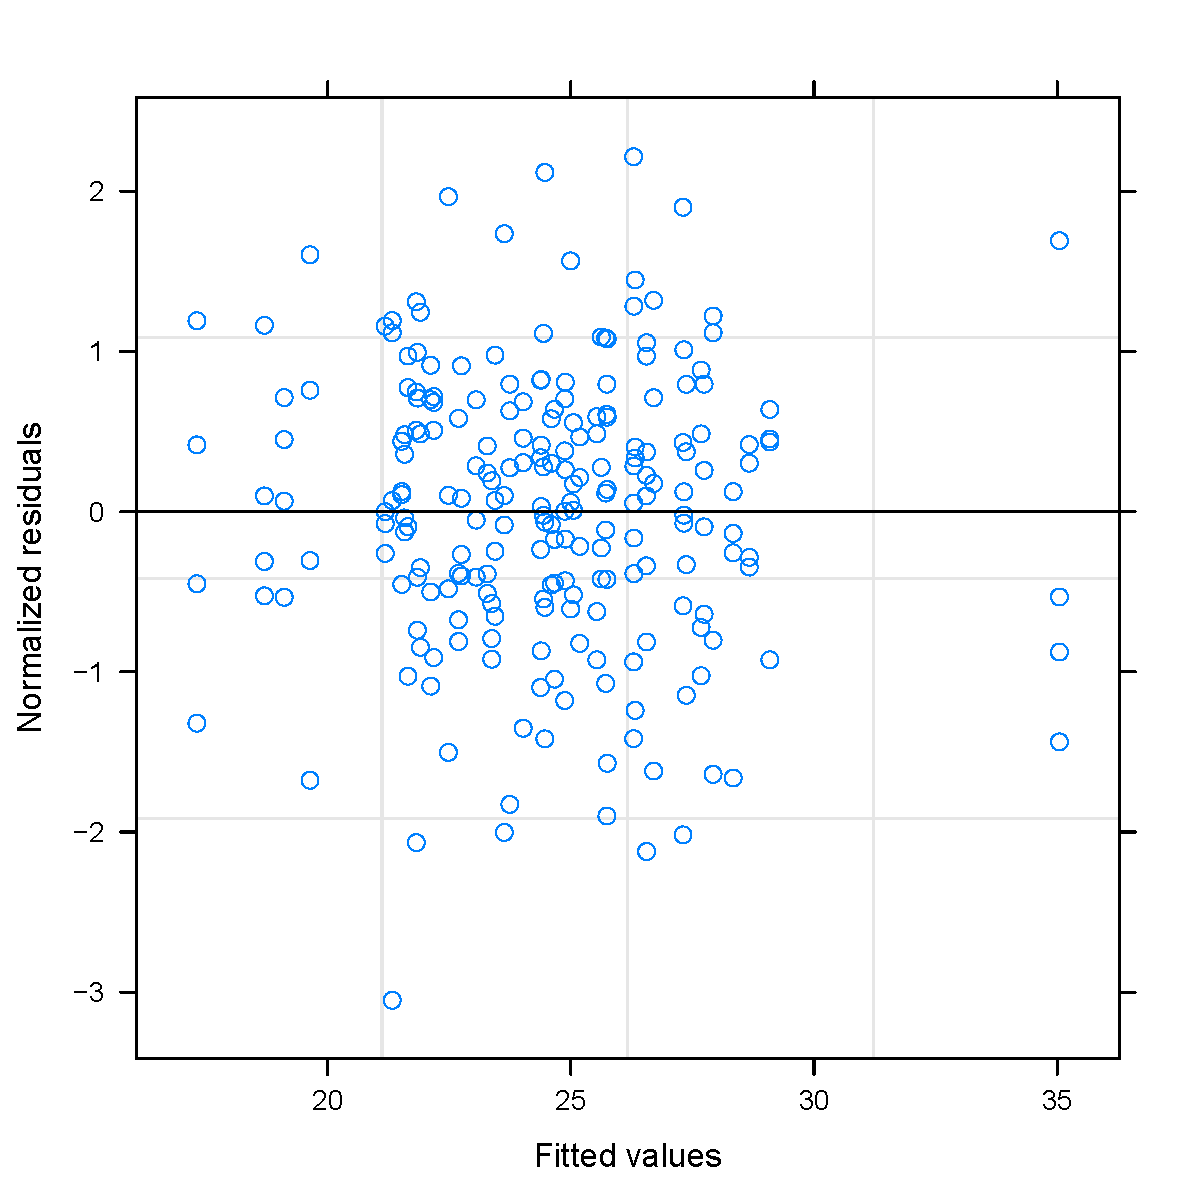
\includegraphics[width=0.48\linewidth]{figures/heteroscedasticity} }\subfloat[检查标准化拟合残差后的正态性:横轴表示标准化后的残差值,纵轴表示标准正态分布的分位数\label{fig:model-check2}]{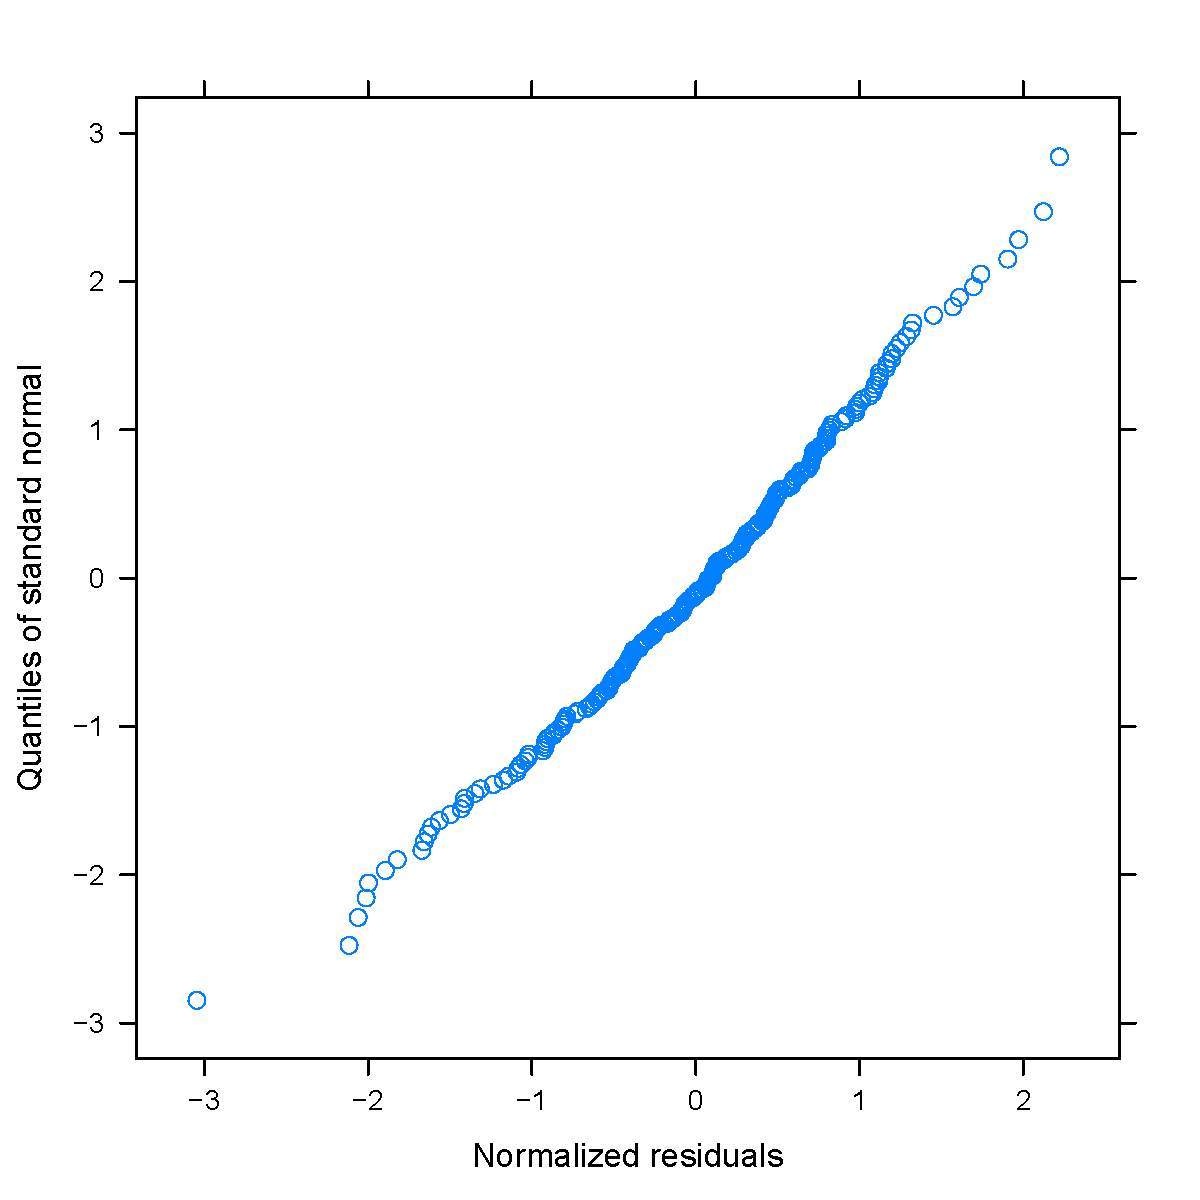
\includegraphics[width=0.48\linewidth]{figures/normality} }

}

\caption{空间线性混合效应模型的拟合残差诊断}\label{fig:model-check}
\end{figure}

值得注意的是,用限制极大似然法估计模型 \eqref{eq:extended-linear-model}
的参数时,对初始值很敏感,通过几番试错调整初值获得如表
\ref{tab:yields-model-compare}
所示结果。根据表\ref{tab:yields-model-compare},
可以得出两个结论,其一选择合适的自相关函数可以取得更好的拟合效果,其二限制极大似然算法对初值很敏感,不断试错以选择合适的初值很重要。最后,再来观察使用空间线性混合效应模型拟合小麦数据后的标准化残差图,如图
\ref{fig:model-check}所示,残差中空间效应已经提取的很充分了。



\hypertarget{case-rongelap}{%
\section{朗格拉普岛核污染浓度的空间分布}\label{case-rongelap}}

朗格拉普岛位于南太平洋上,是马绍尔群岛的一部分,二战后,美国在该岛上进行了多次核武器测试,核爆炸后产生的放射性尘埃笼罩了全岛,目前该岛仍然不适合人类居住,只有经批准的科学研究人员才能登岛。基于马绍尔群岛国家的放射性调查数据,Diggle
等 (1998年) \citep{Diggle1998} 使用
蒙特卡罗极大似然算法估计空间广义线性混合效应模型
\eqref{eq:rongelap-without-nugget-effect} 的各个参数,Christensen
(2004年) \citep{Christensen2004}
发现该核污染数据集中存在不能被泊松分布解释的残差,因此添加了非空间的随机效应
\(Z_i\),建立模型
\eqref{eq:rongelap-with-nugget-effect},在地质统计领域内,\(Z_i\)
还有个专有名词叫块金效应。 \begin{align}
\log\{\lambda(x_{i})\}& =  \beta + S(x_{i}) \label{eq:rongelap-without-nugget-effect}\\
\log\{\lambda(x_{i})\}& =  \beta + S(x_{i}) + Z_{i} \label{eq:rongelap-with-nugget-effect}
\end{align} 放射性调查获得的 rongelap
数据集包含几个观测变量,分别是放射粒子数、相应时间间隔和157个空间坐标。为了增加直观性,绘制图\ref{fig:rongelap-dataset}
展示收集放射性数据的观测站点的空间分布。

\begin{figure}

{\centering 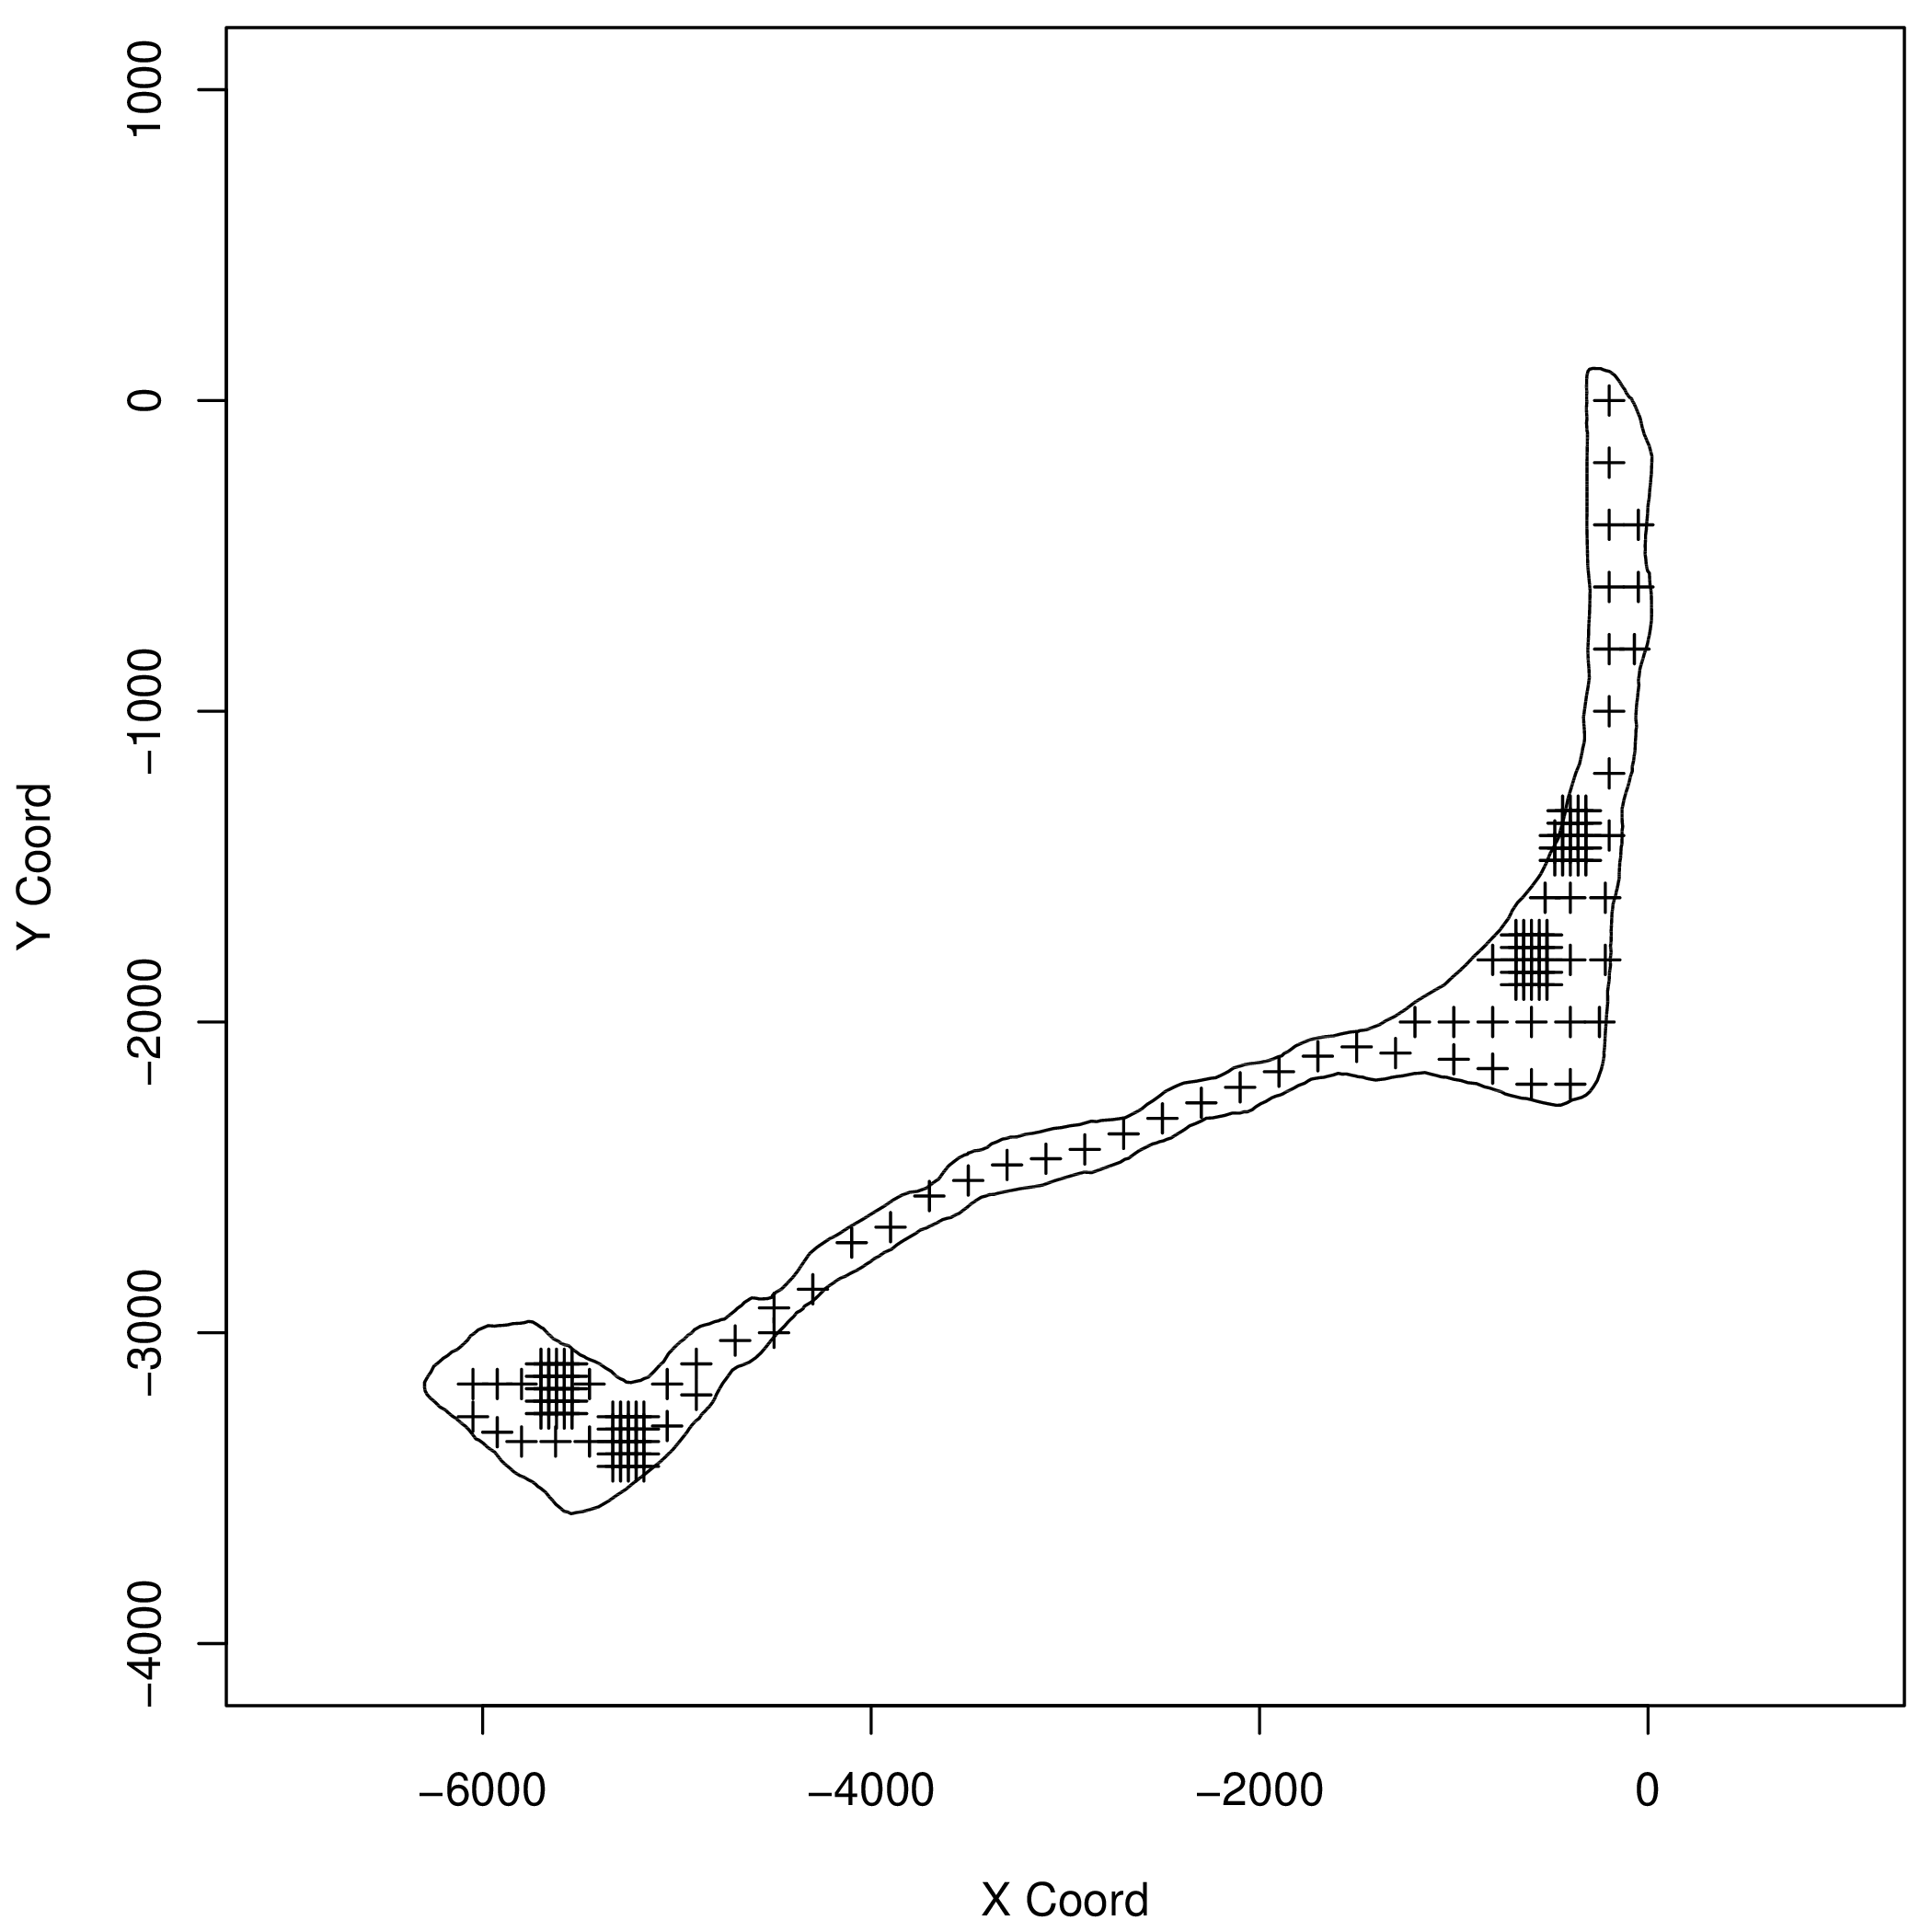
\includegraphics[width=0.65\linewidth]{figures/rongelap-island} 

}

\caption{朗格拉普岛上157个观察测量伽玛粒子放射性强度的站点的空间位置分布,图中加号 + 标注采样的位置,水平方向表示横坐标,垂直方向表示纵坐标,这里使用的坐标系是 UTM (Universal Transverse Mercator) 坐标系}\label{fig:rongelap-dataset}
\end{figure}

根据 \({}^{137}\mathrm{Cs}\) 放出的伽马射线在 \(N=157\)
站点不同时间间隔的放射量, 建立泊松广义线性混合效应模型
\eqref{eq:rongelap-with-nugget-effect}。模型\eqref{eq:rongelap-with-nugget-effect}中,\(\beta\)
是截距, 放射粒子数作为响应变量服从强度为 \(\lambda(x_i)\)
的泊松分布,即
\(Y_{i} \sim \mathrm{Poisson}( \lambda(x_i) )\),平稳空间高斯过程
\(S(x),x \in \mathbb{R}^2\)的自协方差函数为
\(\mathsf{Cov}( S(x_i), S(x_j) ) = \sigma^2 \exp( -\|x_i -x_j\|_{2} / \phi )\),且
\(Z_i\) 之间相互独立同正态分布 \(\mathcal{N}(0,\tau^2)\),这里
\(i = 1,\ldots, 157\)。

蒙特卡罗极大似然算法迭代的初值
\(\beta_{0} = 6.2,\sigma^2_{0} = 2.40,\phi_{0} = 340,\tau^2_{rel} = 2.074\),模拟次数为
30000 次,前 10000 次迭代视为预热阶段 (warm-up),其后每隔 20
次迭代采一个样本点,即存储模型各参数的迭代值,每个参数获得1000次迭代值。蒙特卡罗模拟平稳空间高斯过程
\(S(x)\)
关于响应变量\(Y\)的条件分布时,使用了第\ref{algorithms}章第\ref{sec:MCMC}节介绍的
Langevin-Hastings 算法 \citep{Omiros2003},157 个站点意味着有 157
个条件分布需要模拟,共产生
157个迭代链,每条链需保持平稳才可用于模型参数的推断,因此需要先检验每条链的平稳性,可以采用自相关图和时序图来检验,篇幅所限,取部分站点展示,见附图\ref{fig:rongelap-trace-plot}
和图
\ref{fig:rongelap-acf-plot},经观察157个站点处的\(S_i\)的迭代点列没有出现不平稳的现象。

\begin{longtable}[]{@{}clllll@{}}
\caption{\label{tab:rongelap-mcml-result}
拉普拉斯近似算法(简记LAL)和蒙特卡罗极大似然算法(简记MCL)估计模型
\eqref{eq:rongelap-with-nugget-effect}
的参数,以第4行为例,块金效应的估计值应为
\(\hat{\tau}^2 = \hat{\sigma}^{2} \times \hat{\tau}^2_{rel} = 4.929\)}\tabularnewline
\toprule
\begin{minipage}[b]{0.09\columnwidth}\centering
算法\strut
\end{minipage} & \begin{minipage}[b]{0.15\columnwidth}\raggedright
\(\hat{\beta}(\beta_{0})\)\strut
\end{minipage} & \begin{minipage}[b]{0.15\columnwidth}\raggedright
\(\hat{\sigma}^{2}(\sigma^2_0)\)\strut
\end{minipage} & \begin{minipage}[b]{0.15\columnwidth}\raggedright
\(\hat{\phi}(\phi_0)\)\strut
\end{minipage} & \begin{minipage}[b]{0.15\columnwidth}\raggedright
\(\hat{\tau}^2_{rel}(\tau^2_{rel_0})\)\strut
\end{minipage} & \begin{minipage}[b]{0.15\columnwidth}\raggedright
\(\log L_{m}\)\strut
\end{minipage}\tabularnewline
\midrule
\endfirsthead
\toprule
\begin{minipage}[b]{0.09\columnwidth}\centering
算法\strut
\end{minipage} & \begin{minipage}[b]{0.15\columnwidth}\raggedright
\(\hat{\beta}(\beta_{0})\)\strut
\end{minipage} & \begin{minipage}[b]{0.15\columnwidth}\raggedright
\(\hat{\sigma}^{2}(\sigma^2_0)\)\strut
\end{minipage} & \begin{minipage}[b]{0.15\columnwidth}\raggedright
\(\hat{\phi}(\phi_0)\)\strut
\end{minipage} & \begin{minipage}[b]{0.15\columnwidth}\raggedright
\(\hat{\tau}^2_{rel}(\tau^2_{rel_0})\)\strut
\end{minipage} & \begin{minipage}[b]{0.15\columnwidth}\raggedright
\(\log L_{m}\)\strut
\end{minipage}\tabularnewline
\midrule
\endhead
\begin{minipage}[t]{0.09\columnwidth}\centering
LAL\strut
\end{minipage} & \begin{minipage}[t]{0.15\columnwidth}\raggedright
1.821(2.014)\strut
\end{minipage} & \begin{minipage}[t]{0.15\columnwidth}\raggedright
0.264(0.231)\strut
\end{minipage} & \begin{minipage}[t]{0.15\columnwidth}\raggedright
151.795(50)\strut
\end{minipage} & \begin{minipage}[t]{0.15\columnwidth}\raggedright
0.133(0.1)\strut
\end{minipage} & \begin{minipage}[t]{0.15\columnwidth}\raggedright
\(-1317.195\)\strut
\end{minipage}\tabularnewline
\begin{minipage}[t]{0.09\columnwidth}\centering
MCL\strut
\end{minipage} & \begin{minipage}[t]{0.15\columnwidth}\raggedright
1.821(2.014)\strut
\end{minipage} & \begin{minipage}[t]{0.15\columnwidth}\raggedright
0.265(0.231)\strut
\end{minipage} & \begin{minipage}[t]{0.15\columnwidth}\raggedright
151.859(50)\strut
\end{minipage} & \begin{minipage}[t]{0.15\columnwidth}\raggedright
0.132(0.1)\strut
\end{minipage} & \begin{minipage}[t]{0.15\columnwidth}\raggedright
\(-8.8903\)\strut
\end{minipage}\tabularnewline
\begin{minipage}[t]{0.09\columnwidth}\centering
MCL\strut
\end{minipage} & \begin{minipage}[t]{0.15\columnwidth}\raggedright
6.190(6.200)\strut
\end{minipage} & \begin{minipage}[t]{0.15\columnwidth}\raggedright
2.401(2.400)\strut
\end{minipage} & \begin{minipage}[t]{0.15\columnwidth}\raggedright
338.126(340)\strut
\end{minipage} & \begin{minipage}[t]{0.15\columnwidth}\raggedright
2.053(2.074)\strut
\end{minipage} & \begin{minipage}[t]{0.15\columnwidth}\raggedright
\(-5.8458\)\strut
\end{minipage}\tabularnewline
\bottomrule
\end{longtable}

表 \ref{tab:rongelap-mcml-result} 中括号内表示相应参数的初值,第 2
行是基于第\ref{algorithms}章第\ref{subsec:LA}小节
介绍的拉普拉斯近似算法获得的结果,第 3
行基于蒙特卡罗极大似然算法获得的结果,其初值选择和拉普拉斯近似算法一致,第
4
行先根据剖面似然轮廓图\ref{fig:profile-phi-tausq}确定初值,然后根据蒙特卡罗极大似然算法获得参数估计值。第6列是最终参数估计值处的对数似然函数值,由于两个算法所采用的方法不同,前者采用拉普拉斯近似似然函数中的高维积分,并且扔掉了似然函数中的正则常数,后者采用蒙特卡罗模拟计算高维积分,所以对数似然函数值差别很大,两种算法之间不能以这个比较算法优劣。表\ref{tab:rongelap-mcml-result}第3和第4行的设置是同种算法不同初始值的比较,可以比较最终的似然函数值,后者初值选得好,对数似然函数值更大,同时结合图
\ref{fig:profile-phi-tausq}
有理由怀疑前一组初值使得最终的迭代陷入一个局部极值点或者由于似然曲面太平坦致使迭代停止。

\begin{figure}[!htb]

{\centering 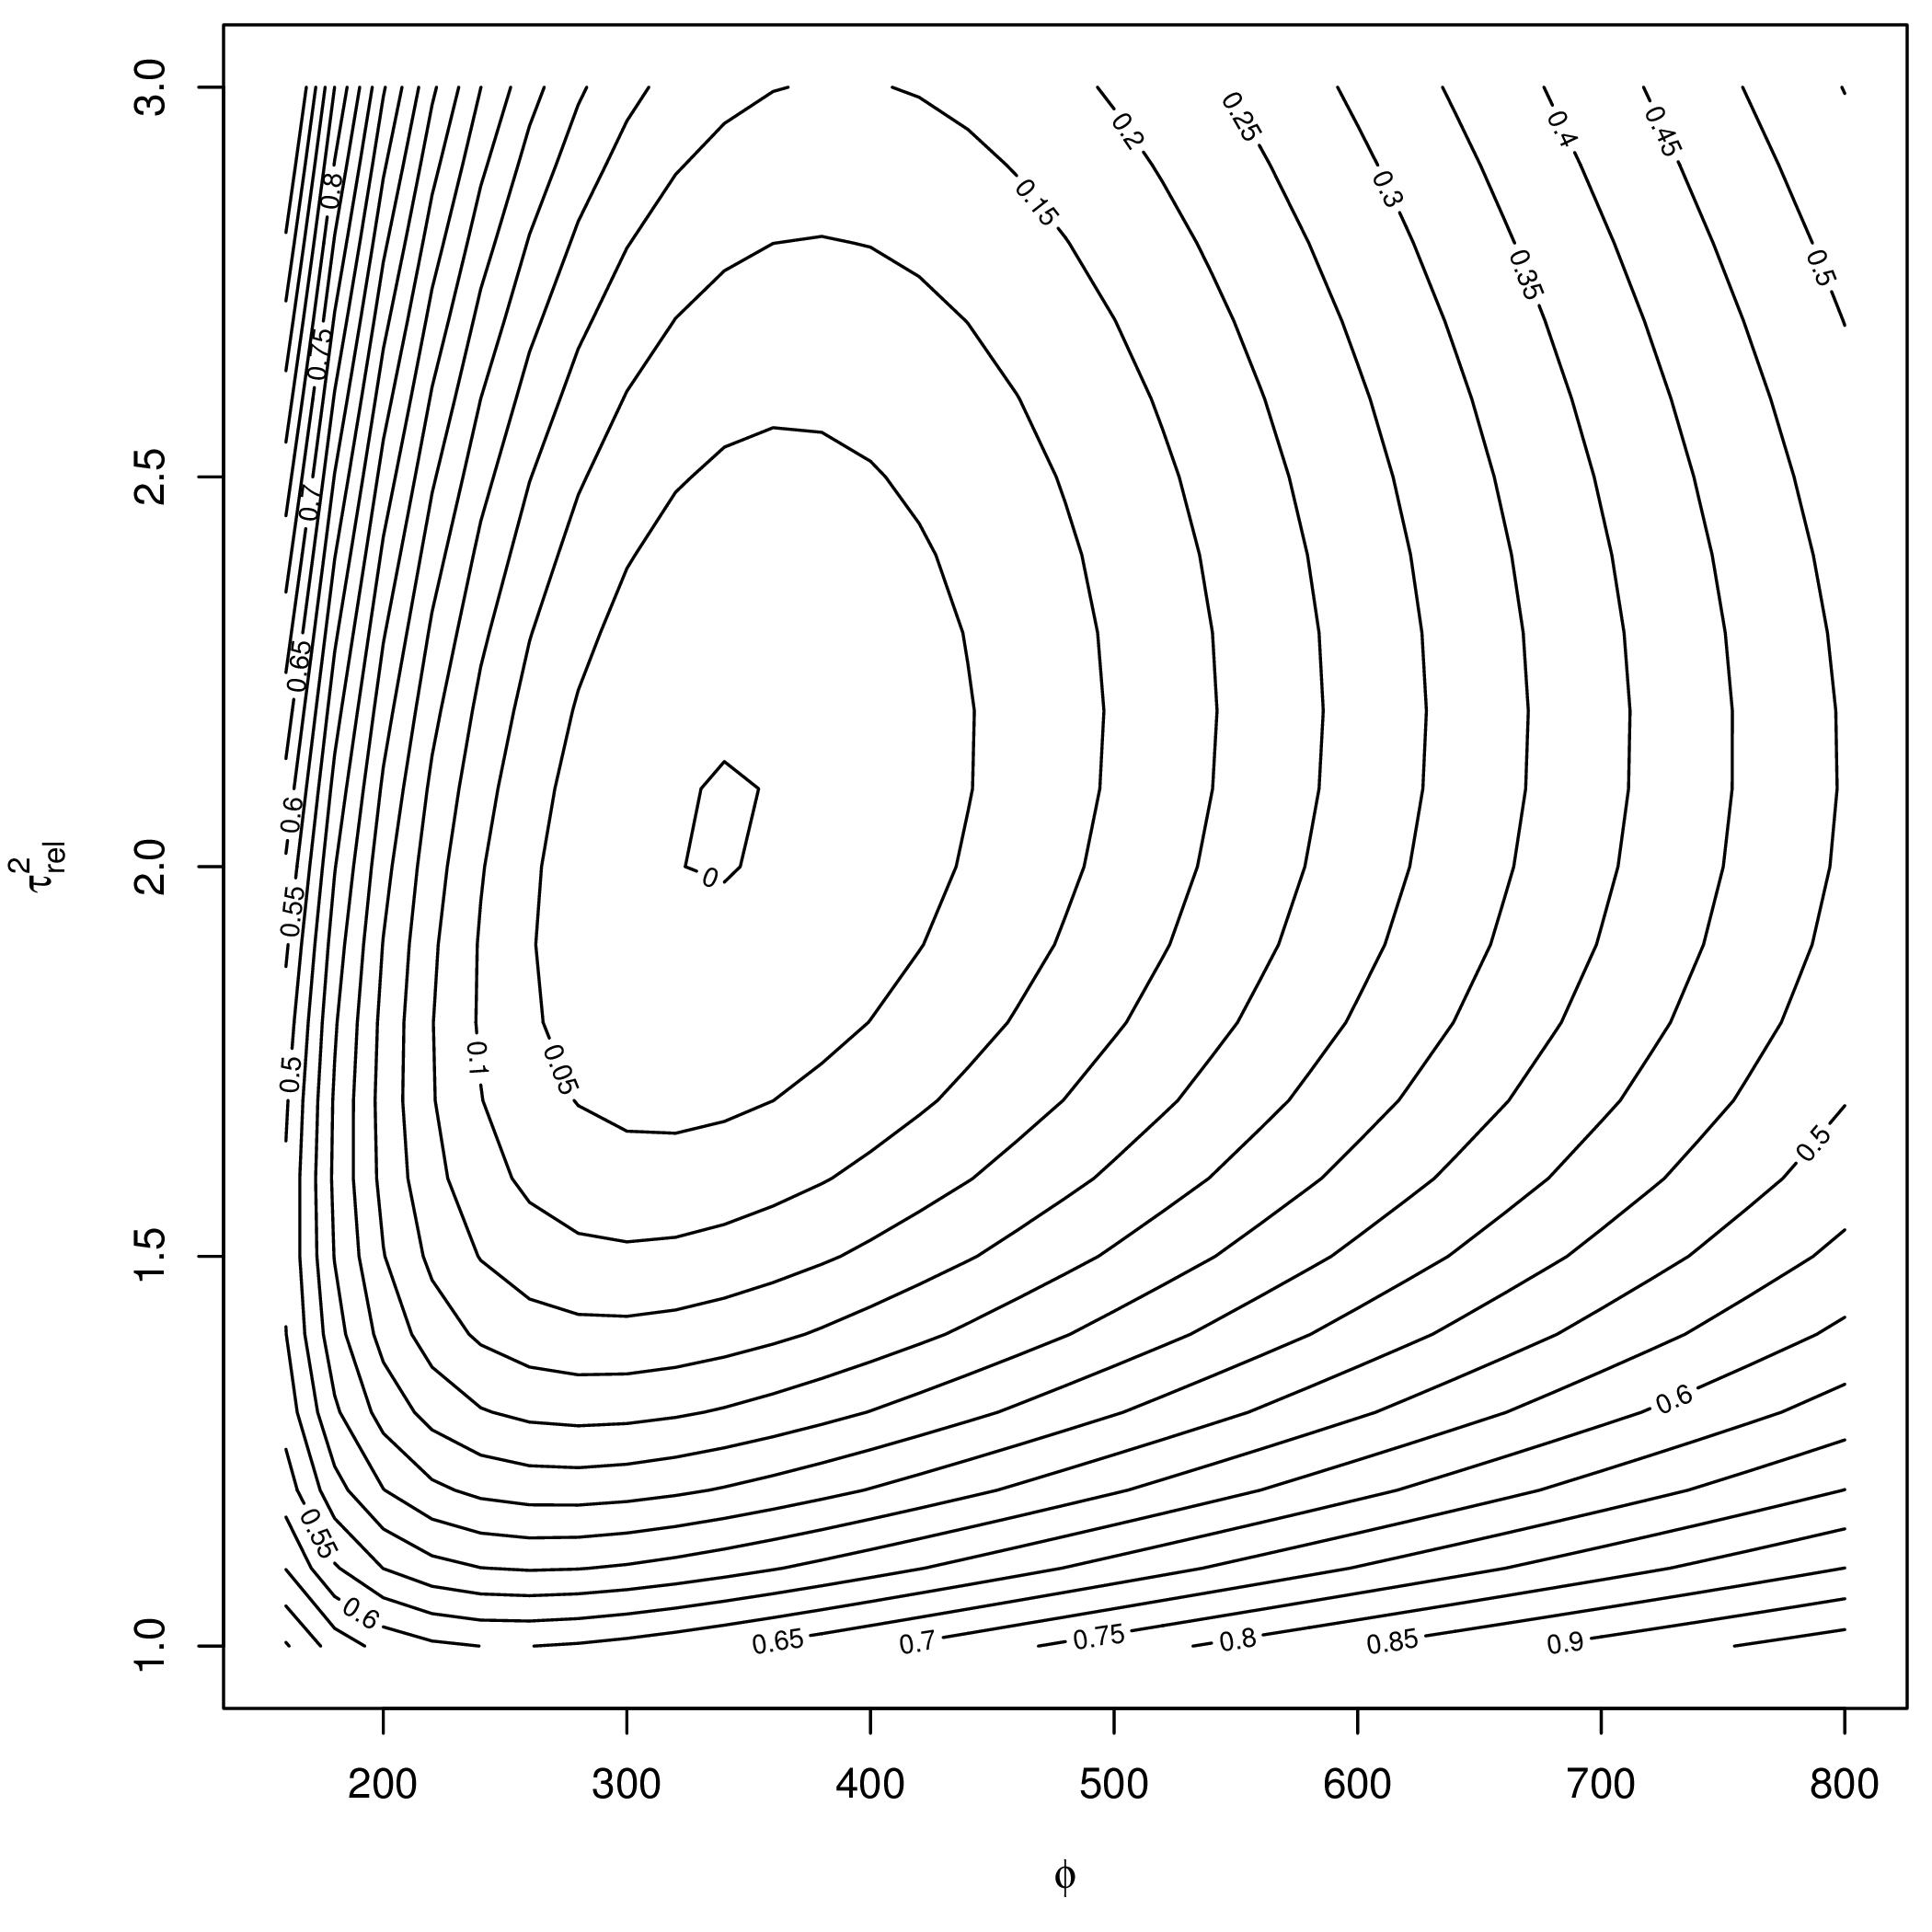
\includegraphics[width=0.65\linewidth]{figures/profile-phitausq} 

}

\caption{泊松型空间广义线性混合效应模型
\eqref{eq:rongelap-with-nugget-effect} 关于 \(\phi\) 和相对块金效应
\(\tau^2_{rel} = \tau^2 / \sigma^2\)
的剖面似然函数曲面,平稳空间高斯过程 \(S(x)\) 的自协方差函数选用指数型
\(\mathsf{Cov}( S(x_i), S(x_j) ) = \sigma^2 \exp( -\|x_i -x_j\|_{2} / \phi )\),剖面似然函数值由
geoRglm 包提供的 proflik.glsm 函数计算}\label{fig:profile-phi-tausq}
\end{figure}

由表 \ref{tab:rongelap-mcml-result} 可知,正如第 \ref{simulations} 章第
\ref{sec:simulations}
节对蒙特卡罗极大似然算法所指出的那样,必须提供足够接近真值的初值,才能获得好的参数估计。由图
\ref{fig:profile-phi-tausq} 不难看出,关于 \(\phi\) 和相对块金效应
\(\tau^2_{rel}\)
的剖面似然函数曲面类似一个极其狭长的、坡度又平缓的山谷,基于似然的算法对这种类型的问题还没有好的解决办法,目前取多个不同参数初值进行迭代,用迭代值画出剖面似然函数曲面,然后通过观察获得最佳初值。从实践的过程来看,参数初值的组数不宜太多,过多可能会用掉不少计算资源,因为如第\ref{algorithms}章第\ref{sec:profile-likelihood}节剖面似然估计所指出的迭代过程,剖面似然函数值的计算涉及空间随机效应的协方差阵的求逆,当空间采样点数目较多时,协方差阵阶数会随着变大,计算会变困难。








\hypertarget{sec:cases}{%
\section{本章小结}\label{sec:cases}}

从小麦数据和核污染数据的似然分析中,可以清晰地看到模型参数初值对求似然函数极值点的重要性。借助变差图等可视化手段探索模型结构,确定初值是很有意义的,在小麦数据的分析过程中,并不是一步到位地给出空间线性混合效应模型,而是给出了模型从简单到复杂的建模过程,这对于实际应用有指导意义。对核残留数据集,建立了泊松型空间广义线性混合效应模型,其似然分析则借助了剖面似然估计的思想,将一个含有多个参数的未知似然函数降至只有两维的剖面似然函数曲面,再对似然曲面的分析获得最佳初始值的位置,最后根据蒙特卡罗最大似然算法获得了近似全局最优的参数估计值。

\hypertarget{summary}{%
\chapter{总结与展望}\label{summary}}

本文重点研究了估计空间广义线性混合效应模型参数的算法,包括蒙特卡罗最大似然算法、低秩近似算法、贝叶斯
MCMC 算法和贝叶斯 STAN-MCMC 算法。在相同设置下,模拟实验中贝叶斯
STAN-MCMC 算法相比贝叶斯 MCMC
算法获得了很大的优势,在估计差不多的情形下,前者迭代次数比后者少很多,而且也不用复杂而耗时的调参,这对于实际应用很有帮助。但是
Stan
编程需要较多的技巧,不仅要熟悉统计模型,还需要了解模型编译的过程,特别是在发生错误和迭代不收敛的情况下,能够根据
Stan
提供的提示修改程序。空间广义线性混合效应模型的似然分析,包括拉普拉斯似然和蒙特卡罗似然都对参数初值比较敏感,结合剖面似然曲面分析是很重要的。

Rue 等 (2009 年) \citep{Rue2009} 提出集成嵌套拉普拉斯 (Integrated
Nested Laplace Approximations,简称 INLA)
算法做近似贝叶斯推断,其广泛的适应性和高效性受到越来越多的关注,还有快速发展的
\href{http://www.r-inla.org/}{INLA 社区},配套程序库 R-INLA
在不断的更新,基于这些因素,未来可以比较 INLA 和 Stan
在空间广义线性混合效应模型下的表现。

贝叶斯方法的在近些年的兴起,离不开现代计算机的贡献,计算力越来越强劲,蒙特卡罗方法出现在越来越多的软件和程序库中,特别是
Stan,目前最新版的 Stan
已经具有一定的规模并行能力,这对于推动贝叶斯理论和应用是非常有帮助的。目前,Stan
程序库在 GPU
上的并行计算已经列入\href{https://github.com/stan-dev/stan/wiki/Longer-Term-To-Do-List}{开发日程}。

\setlength{\bibsep}{0ex}
\bibliography{latex/refer.bib,latex/book.bib}
\addcontentsline{toc}{chapter}{\bibname}

\chapter*{\markboth{致谢}{致谢}{致\quad 谢}}
\addcontentsline{toc}{chapter}{致谢}

三年时间说短不短,说长不长,但是对我却是意义重大的三年,无论是学习还是生活,学校对我的影响都是终生难忘的。首先,我要感谢父母一如既往的默默支持,没有他们就没有我的今天,虽然远隔千山万里,也照顾不到我的学习和生活,但只要想到不管我做怎样的决定,他们都会全力支持,我很感动。

然后,我要感谢我的导师李再兴教授,从他那里我学到严谨治学的态度,感谢他三年来细心的指导,在我论文遇到困难的时候给予了关键的帮助。除了在学校的学习,导师也让我去一些技术公司实习,接触到最前沿的正在发生深刻变革的人工智能领域,这段实习经历除了让我开阔眼界,接触了深度学习技术和计算框架,更重要的是结识了老师木和一些志同道合的同事,如深度学习算法研究者陈新鹏,计算框架开发者王笑舒等;此外,还要感谢新浪的总监高鹏,实习期间,除了基本业务外,让我做了很多我感兴趣的事,如学习
R 语言绘图系统和 R Markdown 生态系统,这让我后来决定基于 R Markdown
写了这篇论文;接着,我要感谢 Stan 开发团队,特别是 R 包 \textbf{brms}
的创建者和维护者 Paul Bürkner,基于他的工作我实现了论文当中的 STAN-MCMC
算法。

最后我要感谢统计之都, 特别是创始人谢益辉,
除了使用他开发的工具打造毕业论文模板,使得论文排版工作量大大减轻,一年多以来,还一直对我的问题有问必答。三年来,帮助过我的老师,同学,同事,朋友太多,他们当中很多都直接或间接地帮助了我的毕业论文,人生最大的幸运莫过于结识你们。

\hypertarget{author}{%
\chapter*{作者简介}\label{author}}
\addcontentsline{toc}{chapter}{作者简介}

\chaptermark{作者简介}

黄湘云,男(1992-),2015年毕业于中国矿业大学(北京),获理学学位;2018年毕业于中国矿业大学(北京),攻读硕士学位,专业为统计学,研究方向为数据分析与统计计算。

\begin{center} \kaishu \zihao{4}{{在学期间参加科研项目}}\end{center}

\begin{enumerate}
\def\labelenumi{\arabic{enumi}.}
\tightlist
\item
  国家自然科学基金面上项目``混合模型的方差元素检验及函数型混合模型研究''参加。项目编号:11671398。2017年1月-2020年12月。
\end{enumerate}

\begin{center} \kaishu \zihao{4}{{主要获奖}}\end{center}

\begin{enumerate}
\def\labelenumi{\arabic{enumi}.}
\tightlist
\item
  2015-2016 年度获研究生优秀学生一等奖学金
\item
  2016 年第十三届全国研究生数学建模大赛成功参赛奖
\item
  2016-2017 年度获研究生优秀学生二等奖学金
\item
  2016-2017 年度获研究生优秀学生奖学金
\item
  2018 年第一届 bookdown 大赛亚军
\item
  2018 年第十一届中国 R 语言大会北京分会场 30 分钟报告
\end{enumerate}

\cleardoublepage

\chapter*{\markboth{附录}{附录}{附\quad 录}}
\addcontentsline{toc}{chapter}{附录 A}

\hypertarget{tables-simulations}{%
\section*{表格}\label{tables-simulations}}
\addcontentsline{toc}{section}{表格}

\begin{longtable}[]{@{}lrrrrrrrr@{}}
\caption{\label{tab:LH-binom-SGLMM} Langevin-Hastings 算法:模型
\eqref{eq:binom-SGLMM} 中 64 个采样点处概率
\(p(x_i) = \exp[S(x_i)]/\{1 + \exp[S(x_i)]\}\)
的后验分布的均值(mean),方差(variance),标准差(standard deviation)和 5
个分位点,样本量为 1000}\tabularnewline
\toprule
& mean & var & sd & 2.5\% & 25\% & 50\% & 75\% & 97.5\%\tabularnewline
\midrule
\endfirsthead
\toprule
& mean & var & sd & 2.5\% & 25\% & 50\% & 75\% & 97.5\%\tabularnewline
\midrule
\endhead
\(p(x_{1})\) & 0.476 & 0.019 & 0.138 & 0.231 & 0.368 & 0.467 & 0.573 &
0.759\tabularnewline
\(p(x_{2})\) & 0.423 & 0.017 & 0.129 & 0.190 & 0.331 & 0.417 & 0.510 &
0.695\tabularnewline
\(p(x_{3})\) & 0.313 & 0.015 & 0.122 & 0.106 & 0.221 & 0.309 & 0.389 &
0.582\tabularnewline
\(p(x_{4})\) & 0.470 & 0.020 & 0.141 & 0.204 & 0.372 & 0.466 & 0.564 &
0.755\tabularnewline
\(p(x_{5})\) & 0.431 & 0.018 & 0.133 & 0.181 & 0.338 & 0.425 & 0.527 &
0.686\tabularnewline
\(p(x_{6})\) & 0.516 & 0.017 & 0.131 & 0.256 & 0.429 & 0.517 & 0.612 &
0.766\tabularnewline
\(p(x_{7})\) & 0.580 & 0.017 & 0.132 & 0.326 & 0.485 & 0.583 & 0.669 &
0.831\tabularnewline
\(p(x_{8})\) & 0.483 & 0.019 & 0.138 & 0.220 & 0.386 & 0.484 & 0.578 &
0.736\tabularnewline
\(p(x_{9})\) & 0.487 & 0.020 & 0.141 & 0.235 & 0.383 & 0.482 & 0.584 &
0.772\tabularnewline
\(p(x_{10})\) & 0.333 & 0.014 & 0.117 & 0.121 & 0.251 & 0.326 & 0.411 &
0.583\tabularnewline
\(p(x_{11})\) & 0.262 & 0.013 & 0.112 & 0.083 & 0.175 & 0.248 & 0.334 &
0.499\tabularnewline
\(p(x_{12})\) & 0.367 & 0.016 & 0.126 & 0.150 & 0.279 & 0.358 & 0.446 &
0.627\tabularnewline
\(p(x_{13})\) & 0.491 & 0.017 & 0.129 & 0.248 & 0.403 & 0.487 & 0.579 &
0.742\tabularnewline
\(p(x_{14})\) & 0.585 & 0.016 & 0.127 & 0.343 & 0.493 & 0.589 & 0.673 &
0.826\tabularnewline
\(p(x_{15})\) & 0.573 & 0.016 & 0.125 & 0.320 & 0.491 & 0.576 & 0.660 &
0.811\tabularnewline
\(p(x_{16})\) & 0.610 & 0.016 & 0.127 & 0.347 & 0.526 & 0.612 & 0.701 &
0.843\tabularnewline
\(p(x_{17})\) & 0.336 & 0.016 & 0.127 & 0.130 & 0.241 & 0.323 & 0.415 &
0.605\tabularnewline
\(p(x_{18})\) & 0.299 & 0.013 & 0.114 & 0.108 & 0.217 & 0.292 & 0.368 &
0.566\tabularnewline
\(p(x_{19})\) & 0.269 & 0.012 & 0.109 & 0.088 & 0.190 & 0.258 & 0.337 &
0.502\tabularnewline
\(p(x_{20})\) & 0.429 & 0.016 & 0.128 & 0.192 & 0.336 & 0.428 & 0.520 &
0.687\tabularnewline
\(p(x_{21})\) & 0.504 & 0.015 & 0.124 & 0.270 & 0.417 & 0.499 & 0.583 &
0.761\tabularnewline
\(p(x_{22})\) & 0.550 & 0.015 & 0.121 & 0.308 & 0.469 & 0.556 & 0.633 &
0.785\tabularnewline
\(p(x_{23})\) & 0.617 & 0.015 & 0.123 & 0.360 & 0.538 & 0.622 & 0.705 &
0.842\tabularnewline
\(p(x_{24})\) & 0.646 & 0.015 & 0.124 & 0.380 & 0.563 & 0.660 & 0.732 &
0.868\tabularnewline
\(p(x_{25})\) & 0.246 & 0.012 & 0.111 & 0.066 & 0.166 & 0.237 & 0.312 &
0.483\tabularnewline
\(p(x_{26})\) & 0.287 & 0.013 & 0.113 & 0.097 & 0.206 & 0.275 & 0.356 &
0.541\tabularnewline
\(p(x_{27})\) & 0.341 & 0.014 & 0.118 & 0.121 & 0.261 & 0.332 & 0.416 &
0.586\tabularnewline
\(p(x_{28})\) & 0.525 & 0.016 & 0.128 & 0.298 & 0.427 & 0.524 & 0.609 &
0.772\tabularnewline
\(p(x_{29})\) & 0.540 & 0.016 & 0.128 & 0.295 & 0.446 & 0.542 & 0.631 &
0.783\tabularnewline
\(p(x_{30})\) & 0.583 & 0.015 & 0.123 & 0.348 & 0.496 & 0.583 & 0.671 &
0.813\tabularnewline
\(p(x_{31})\) & 0.517 & 0.017 & 0.130 & 0.251 & 0.432 & 0.525 & 0.606 &
0.756\tabularnewline
\(p(x_{32})\) & 0.689 & 0.014 & 0.117 & 0.437 & 0.612 & 0.693 & 0.775 &
0.898\tabularnewline
\(p(x_{33})\) & 0.260 & 0.012 & 0.111 & 0.075 & 0.178 & 0.251 & 0.328 &
0.494\tabularnewline
\(p(x_{34})\) & 0.304 & 0.014 & 0.119 & 0.101 & 0.218 & 0.292 & 0.371 &
0.577\tabularnewline
\(p(x_{35})\) & 0.394 & 0.016 & 0.125 & 0.171 & 0.308 & 0.389 & 0.472 &
0.669\tabularnewline
\(p(x_{36})\) & 0.497 & 0.017 & 0.130 & 0.249 & 0.412 & 0.495 & 0.587 &
0.746\tabularnewline
\(p(x_{37})\) & 0.604 & 0.017 & 0.131 & 0.346 & 0.518 & 0.606 & 0.700 &
0.844\tabularnewline
\(p(x_{38})\) & 0.546 & 0.016 & 0.126 & 0.298 & 0.459 & 0.548 & 0.636 &
0.774\tabularnewline
\(p(x_{39})\) & 0.494 & 0.017 & 0.129 & 0.242 & 0.404 & 0.498 & 0.582 &
0.735\tabularnewline
\(p(x_{40})\) & 0.639 & 0.015 & 0.123 & 0.394 & 0.559 & 0.647 & 0.724 &
0.864\tabularnewline
\(p(x_{41})\) & 0.380 & 0.017 & 0.132 & 0.154 & 0.284 & 0.369 & 0.466 &
0.669\tabularnewline
\(p(x_{42})\) & 0.339 & 0.015 & 0.122 & 0.128 & 0.257 & 0.331 & 0.416 &
0.595\tabularnewline
\(p(x_{43})\) & 0.318 & 0.014 & 0.118 & 0.111 & 0.234 & 0.311 & 0.398 &
0.552\tabularnewline
\(p(x_{44})\) & 0.479 & 0.016 & 0.127 & 0.247 & 0.387 & 0.473 & 0.566 &
0.745\tabularnewline
\(p(x_{45})\) & 0.655 & 0.015 & 0.123 & 0.415 & 0.568 & 0.659 & 0.746 &
0.880\tabularnewline
\(p(x_{46})\) & 0.601 & 0.015 & 0.123 & 0.354 & 0.519 & 0.607 & 0.689 &
0.839\tabularnewline
\(p(x_{47})\) & 0.524 & 0.017 & 0.129 & 0.275 & 0.437 & 0.525 & 0.612 &
0.768\tabularnewline
\(p(x_{48})\) & 0.696 & 0.014 & 0.118 & 0.440 & 0.620 & 0.704 & 0.783 &
0.901\tabularnewline
\(p(x_{49})\) & 0.353 & 0.015 & 0.124 & 0.122 & 0.266 & 0.348 & 0.433 &
0.615\tabularnewline
\(p(x_{50})\) & 0.493 & 0.017 & 0.132 & 0.254 & 0.402 & 0.492 & 0.584 &
0.760\tabularnewline
\(p(x_{51})\) & 0.379 & 0.014 & 0.120 & 0.160 & 0.293 & 0.374 & 0.460 &
0.619\tabularnewline
\(p(x_{52})\) & 0.378 & 0.016 & 0.128 & 0.135 & 0.282 & 0.376 & 0.470 &
0.620\tabularnewline
\(p(x_{53})\) & 0.591 & 0.015 & 0.124 & 0.345 & 0.512 & 0.591 & 0.678 &
0.834\tabularnewline
\(p(x_{54})\) & 0.521 & 0.017 & 0.132 & 0.244 & 0.432 & 0.531 & 0.613 &
0.773\tabularnewline
\(p(x_{55})\) & 0.566 & 0.016 & 0.125 & 0.305 & 0.480 & 0.573 & 0.654 &
0.789\tabularnewline
\(p(x_{56})\) & 0.703 & 0.014 & 0.120 & 0.449 & 0.622 & 0.711 & 0.794 &
0.900\tabularnewline
\(p(x_{57})\) & 0.494 & 0.019 & 0.137 & 0.235 & 0.400 & 0.495 & 0.587 &
0.762\tabularnewline
\(p(x_{58})\) & 0.606 & 0.019 & 0.139 & 0.328 & 0.515 & 0.608 & 0.702 &
0.857\tabularnewline
\(p(x_{59})\) & 0.482 & 0.018 & 0.133 & 0.236 & 0.387 & 0.478 & 0.575 &
0.725\tabularnewline
\(p(x_{60})\) & 0.443 & 0.017 & 0.130 & 0.195 & 0.349 & 0.447 & 0.536 &
0.695\tabularnewline
\(p(x_{61})\) & 0.636 & 0.015 & 0.124 & 0.390 & 0.547 & 0.638 & 0.723 &
0.867\tabularnewline
\(p(x_{62})\) & 0.620 & 0.015 & 0.122 & 0.371 & 0.537 & 0.623 & 0.708 &
0.843\tabularnewline
\(p(x_{63})\) & 0.568 & 0.016 & 0.128 & 0.321 & 0.470 & 0.571 & 0.660 &
0.802\tabularnewline
\(p(x_{64})\) & 0.633 & 0.017 & 0.131 & 0.354 & 0.545 & 0.644 & 0.729 &
0.861\tabularnewline
\bottomrule
\end{longtable}

\begin{longtable}[]{@{}lrrrrrrrrrr@{}}
\caption{\label{tab:HMC-Pois-SGLMM} 汉密尔顿蒙特卡罗算法,采样点 64
个,泊松空间模型参数 \(\alpha,\phi,\sigma^2\)
的估计值,后验均值(mean)、蒙特卡罗误差 (se\_mean)、后验标准差
(sd)、5个后验分位点等}\tabularnewline
\toprule
& mean & se\_mean & sd & 2.5\% & 25\% & 50\% & 75\% & 97.5\% & n\_eff &
Rhat\tabularnewline
\midrule
\endfirsthead
\toprule
& mean & se\_mean & sd & 2.5\% & 25\% & 50\% & 75\% & 97.5\% & n\_eff &
Rhat\tabularnewline
\midrule
\endhead
\(\alpha\) & 0.50 & 0.02 & 0.63 & -0.77 & 0.08 & 0.53 & 0.92 & 1.80 &
1000.00 & 1.00\tabularnewline
\(\phi\) & 0.39 & 0.00 & 0.06 & 0.28 & 0.34 & 0.38 & 0.42 & 0.51 &
777.31 & 1.00\tabularnewline
\(\sigma^2\) & 2.47 & 0.02 & 0.54 & 1.59 & 2.10 & 2.42 & 2.80 & 3.73 &
1000.00 & 1.00\tabularnewline
lp\_\_ & 722.28 & 0.39 & 6.83 & 708.00 & 718.14 & 722.49 & 726.91 &
734.71 & 312.69 & 1.03\tabularnewline
\bottomrule
\end{longtable}

\hypertarget{simulate-plot}{%
\section*{图}\label{simulate-plot}}
\addcontentsline{toc}{section}{图}

\begin{figure}

{\centering 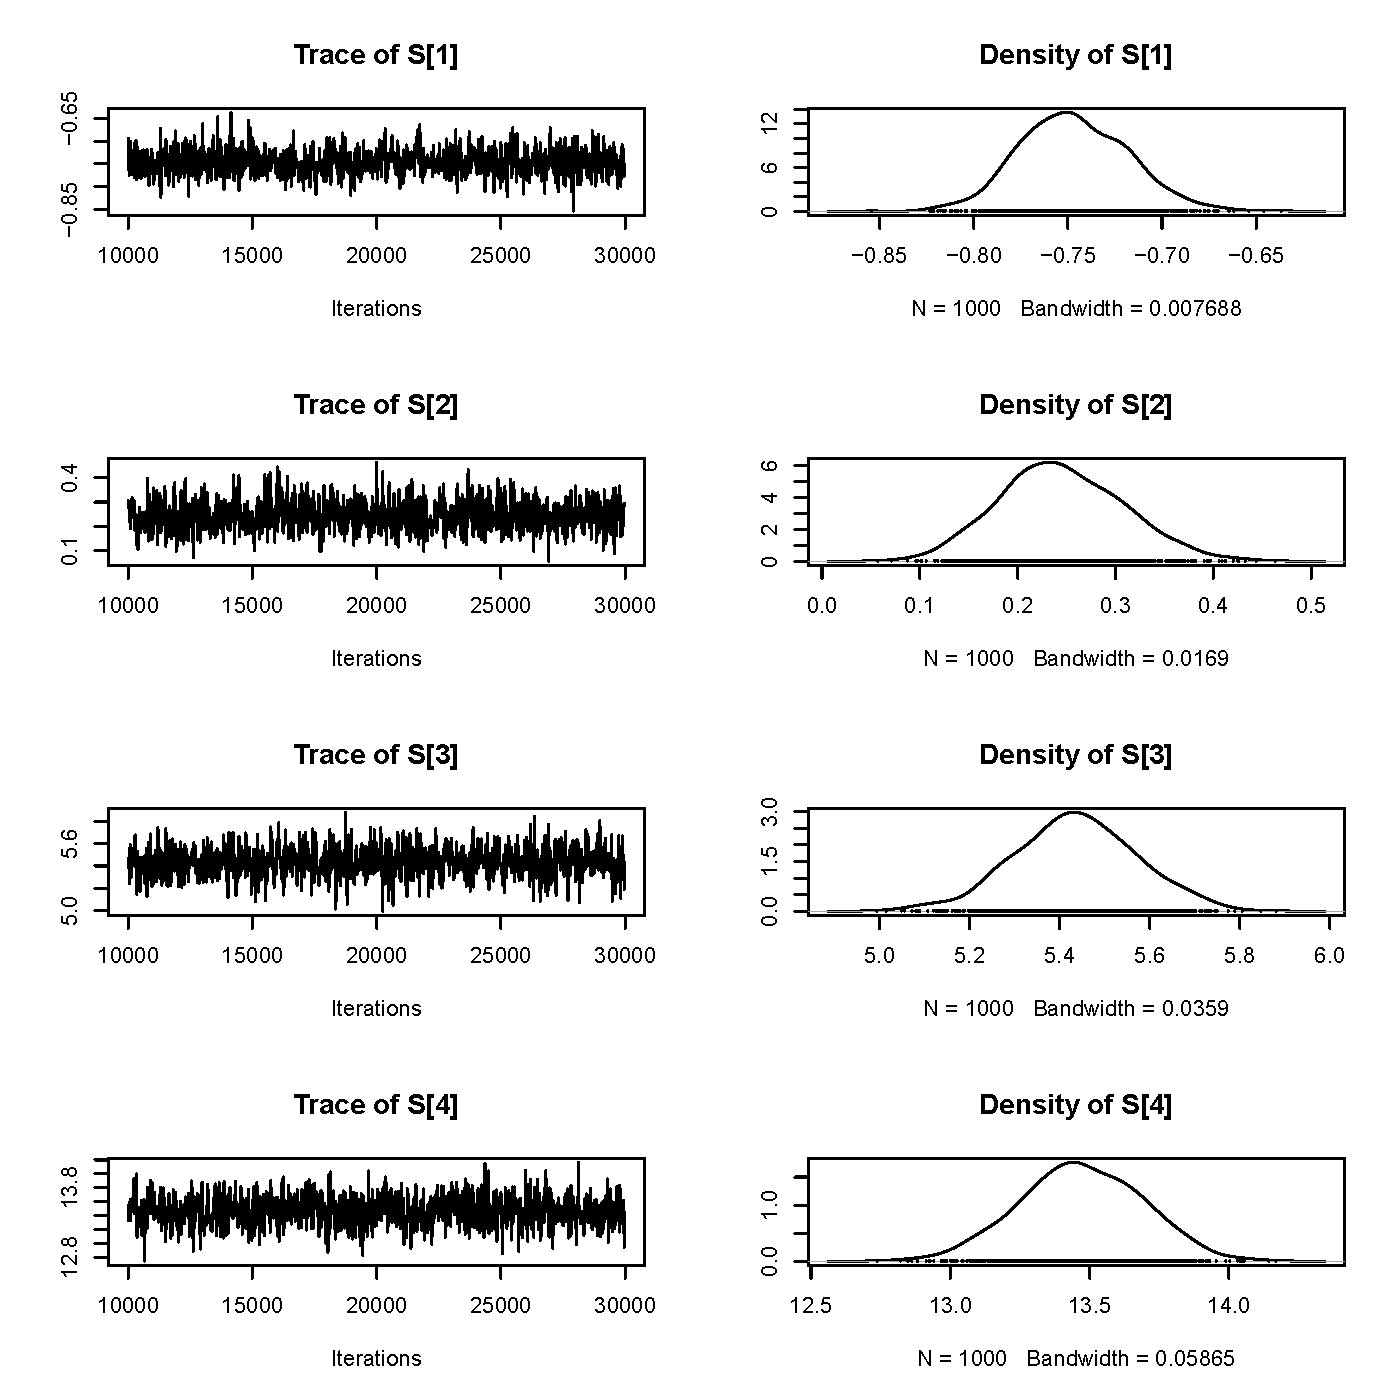
\includegraphics[width=0.7\linewidth]{figures/rongelap-mcml-diagnosis-trace-9} 

}

\caption{Langevin-Hastings 算法模拟条件分布
\([S(x_{i})|Y_{i}], i = 1,\ldots,4\),\([\cdot]\)
表示某某的分布,第一列是迭代序列轨迹图,第二列是对应的密度分布}\label{fig:rongelap-trace-plot}
\end{figure}

从图 \ref{fig:rongelap-trace-plot} 可以看出迭代序列符合平稳性的特征。

\begin{figure}

{\centering 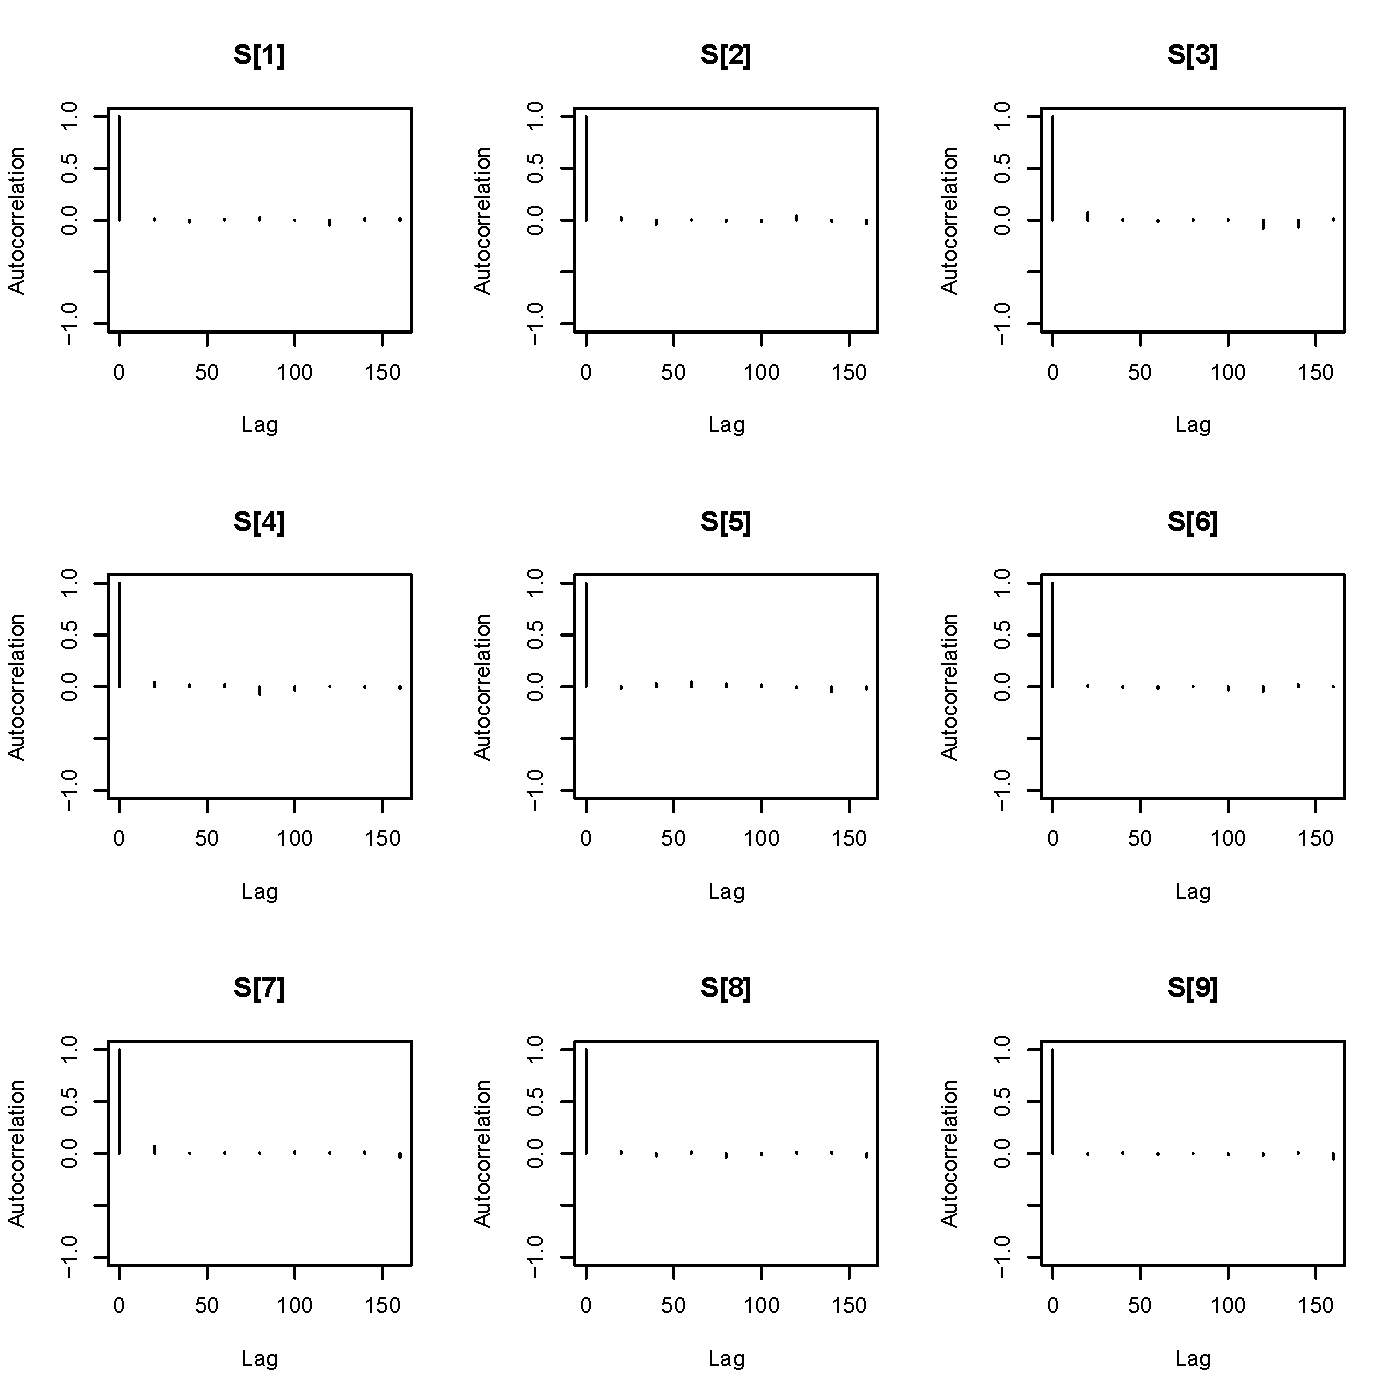
\includegraphics[width=0.7\linewidth]{figures/rongelap-mcml-diagnosis-acf-9} 

}

\caption{条件分布 \([S(x_{i})|Y_{i}], i = 1, \ldots, 4\)
的采样序列的自相关图}\label{fig:rongelap-acf-plot}
\end{figure}

从图 \ref{fig:rongelap-acf-plot}
可以看出迭代序列满足马尔科夫性,没有明显的延迟相关性。








\hypertarget{simulate-code}{%
\section*{代码}\label{simulate-code}}
\addcontentsline{toc}{section}{代码}

模拟平稳空间高斯过程

\begin{verbatim}
// Sample from a Gaussian process using exponentiated covariance function.
// Fixed kernel hyperparameters: phi=0.15, sigma=sqrt(1)

data {
  int<lower=1> N;
  real<lower=0> phi;
  real<lower=0> sigma;
}
transformed data {
  vector[N] zeros;
  zeros = rep_vector(0, N);
}
model {}
generated quantities {
  real x[N];
  vector[N] f;
  for (n in 1:N)
    x[n] = uniform_rng(-2,2);
  {
    matrix[N, N] cov;
    matrix[N, N] L_cov;
    
   // cov = cov_exp_quad(x, sigma, phi);

    for (i in 1:(N - 1)) {
      cov[i, i] = square(sigma);
      for (j in (i + 1):N) {
        cov[i, j] = square(sigma) * exp(- fabs(x[i] - x[j]) * inv(phi));
        cov[j, i] = cov[i, j];
      }
    }
    cov[N, N] = square(sigma); 
    
    for (n in 1:N)
      cov[n, n] = cov[n, n] + 1e-12;

    L_cov = cholesky_decompose(cov);
    f = multi_normal_cholesky_rng(zeros, L_cov);
  }
}
\end{verbatim}

模拟空间广义线性模型

\begin{verbatim}
generate_sim_data <- function(N = 49, intercept = -1.0, 
                              slope1 = 1.0, slope2 = 0.5,
                              lscale = 1, sdgp = 1, 
                              cov.model = "exp_quad", type = "binomal") {
  # set.seed(2018) 
  ## 单位区域上采样
  d <- expand.grid(
    d1 = seq(0, 1, l = sqrt(N)),
    d2 = seq(0, 1, l = sqrt(N))
  )
  D <- as.matrix(dist(d)) # 计算采样点之间的欧氏距离
  switch (cov.model,
          matern = {
            phi = lscale
            corr_m = geoR::matern(D, phi = phi, kappa = 2) # 固定的 kappa = 2 
            m  = sdgp^2 * corr_m 
          },
          exp_quad = {
            phi <- 2 * lscale^2
            m <- sdgp^2 * exp(-D^2 / phi) # 多元高斯分布的协方差矩阵
          }
  )
  # powered.exponential (or stable)
  # rho(h) = exp[-(h/phi)^kappa] if 0 < kappa <= 2 此处 kappa 固定为 2
  S <- MASS::mvrnorm(1, rep(0, N), m) # 产生服从多元高斯分布的随机数
  # 模拟两个固定效应
  x1 <- rnorm(N, 0, 1)
  x2 <- rnorm(N, 0, 4)
  switch(type,
         binomal = {
           units.m <- rep(100, N) # N 个 100
           pred <- intercept + slope1 * x1 + slope2 * x2 + S
           mu <- exp(pred) / (1 + exp(pred))
           y <- rbinom(N, size = 100, prob = mu) # 每个采样点抽取100个样本
           data.frame(d, y, units.m, x1, x2)
         },
         poisson = {
           pred <- intercept + slope1 * x1 + slope2 * x2 + S
           y <- rpois(100, lambda = exp(pred)) # lambda 是泊松分布的期望  
           # Y ~ Possion(lambda) g(u) = ln(u) u = lambda = exp(g(u))
           data.frame(d, y, x1, x2)
         }
  )
}
\end{verbatim}

HMC 算法

\begin{verbatim}
# 加载程序包
library(rstan)
library(brms)
# 以并行方式运行 STAN-MCMC 算法,指定 CPU 的核心数
options(mc.cores = parallel::detectCores())
# 将编译后的模型写入磁盘,可防止重新编译
rstan_options(auto_write = TRUE)
theme_set(theme_default())
prior <- c(
  set_prior("normal(0,10)", class = "b"), # 均值0 标准差 10 的先验
  set_prior("lognormal(0,1)", class = "lscale"),
  set_prior("lognormal(0,1)", class = "sdgp")
)
sim_binom_data <- generate_sim_data(type = "binomal")
benchmark.binomal <- microbenchmark::microbenchmark({
  fit.binomal <- brm(y | trials(units.m) ~ 0 + intercept + x1 + x2 + gp(d1, d2),
    sim_binom_data,
    prior = prior,
    chains = 4, thin = 5, iter = 15000, warmup = 5000,
    algorithm = "sampling", family = binomial()
  )
}, times = 10L)
summary(fit.binomal)

sim_poisson_data <- generate_sim_data(type = "poisson")
benchmark.poisson <- microbenchmark::microbenchmark({
  fit.poisson <- brm(y ~ 0 + intercept + x1 + x2 + gp(d1, d2),
    sim_poisson_data,
    prior = prior,
    chains = 4, thin = 5, iter = 15000, warmup = 5000, 
    algorithm = "sampling", family = poisson()
  )
}, times = 10L)
summary(fit.poisson)
plot(fit.poisson)
\end{verbatim}


\backmatter
% \printindex

\end{document}
